% =====================================================================
%  Term project report -- Microfluidics
%  Shear stress and oxygen transport in a widening Hele-Shaw chip
%  Compile:  latexmk -pdf main.tex   (pdflatex + bibtex)
% =====================================================================
\documentclass[11pt,a4paper,oneside]{report}

% ---------------------------------------------------------------- packages
\usepackage[T1]{fontenc}
\usepackage[utf8]{inputenc}
\usepackage{lmodern}
\usepackage{microtype}
\usepackage[a4paper,left=25mm,right=25mm,top=25mm,bottom=25mm,headheight=14pt]{geometry}
\usepackage{setspace}
\setstretch{1.12}
\usepackage{amsmath,amssymb,mathtools,bm}
\usepackage{graphicx}
\usepackage{booktabs,tabularx,longtable,multirow,makecell,array}
\usepackage{float}
\usepackage[font=small,labelfont=bf,margin=4mm]{caption}
\usepackage{subcaption}
\usepackage[dvipsnames,table]{xcolor}
\usepackage{siunitx}
\sisetup{separate-uncertainty=true, range-phrase=--, per-mode=symbol}
\usepackage{enumitem}
\setlist{itemsep=2pt,topsep=4pt}
\usepackage{fancyhdr}
\usepackage{titlesec}
\usepackage{tcolorbox}
\usepackage[numbers,sort&compress]{natbib}
\usepackage[colorlinks=true,linkcolor=MidnightBlue,citecolor=OliveGreen,urlcolor=MidnightBlue]{hyperref}
\usepackage[capitalise,nameinlink]{cleveref}
\crefname{equation}{Eq.}{Eqs.}
\Crefname{equation}{Equation}{Equations}

% ---------------------------------------------------------------- layout
\titleformat{\chapter}[hang]{\normalfont\LARGE\bfseries\color{MidnightBlue}}{\thechapter}{0.8em}{}
\titlespacing*{\chapter}{0pt}{-8pt}{14pt}
\titleformat{\section}{\normalfont\large\bfseries}{\thesection}{0.8em}{}
\titleformat{\subsection}{\normalfont\normalsize\bfseries}{\thesubsection}{0.8em}{}
\setcounter{secnumdepth}{3}
\setcounter{tocdepth}{1}
\numberwithin{equation}{chapter}
\numberwithin{figure}{chapter}
\numberwithin{table}{chapter}

\pagestyle{fancy}
\fancyhf{}
\fancyhead[L]{\small\itshape Shear stress and oxygen transport in a widening Hele-Shaw chip}
\fancyhead[R]{\small\nouppercase{\leftmark}}
\renewcommand{\chaptermark}[1]{\markboth{\chaptername~\thechapter}{}}
\fancyfoot[C]{\small\thepage}
\renewcommand{\headrulewidth}{0.4pt}
\fancypagestyle{plain}{\fancyhf{}\fancyfoot[C]{\small\thepage}\renewcommand{\headrulewidth}{0pt}}

% ---------------------------------------------------------------- macros
\DeclareSIUnit\dyne{dyn}
\DeclareSIUnit\uLmin{\micro\litre\per\minute}
\DeclareSIUnit\dyncm{\dyne\per\centi\metre\squared}
\newcommand{\ulmin}{\si{\uLmin}}
\newcommand{\dyn}{\si{\dyncm}}
\newcommand{\Csat}{C_{\mathrm{sat}}}
\newcommand{\Cb}{\bar C}
\newcommand{\Cbot}{C_{\mathrm{bot}}}
\newcommand{\Ctop}{C_{\mathrm{top}}}
\newcommand{\qmax}{q_{\max}}
\newcommand{\Km}{K_{m}}
\newcommand{\kp}{k_{\mathrm{PDMS}}}
\newcommand{\taw}{\tau_{w}}
\newcommand{\dd}{\mathrm{d}}
\newcommand{\vect}[1]{\bm{#1}}
\newcommand{\Pe}{\mathit{Pe}}
\newcommand{\Rey}{\mathit{Re}}
\newcommand{\Da}{\mathit{Da}}
\newcommand{\Bi}{\mathit{Bi}}
\newcommand{\Sh}{\mathit{Sh}}
% source tags used throughout the report
\newcommand{\tagP}{\textsuperscript{[P]}}   % published (Delon et al. 2020)
\newcommand{\tagC}{\textsuperscript{[C]}}   % our CFD
\newcommand{\tagT}{\textsuperscript{[T]}}   % theory derived here
\newcommand{\tagM}{\textsuperscript{[M]}}   % model estimate (reduced-order / assumed parameters)
\newtcolorbox{keybox}[1][]{colback=MidnightBlue!4,colframe=MidnightBlue!60,boxrule=0.5pt,arc=1mm,left=2mm,right=2mm,top=1mm,bottom=1mm,fonttitle=\bfseries\small,title=#1}

\graphicspath{{figures/}}

% =====================================================================
\begin{document}

\begin{titlepage}
\centering
\vspace*{8mm}
{\large\scshape Microfluidics \textendash{} Term Project Report\par}
\vspace{2mm}
{\normalsize Course code: CLL770 \quad Instructor: \texttt{[instructor name]}\par}
\vspace{18mm}
{\color{MidnightBlue}\rule{\linewidth}{1pt}\par}
\vspace{5mm}
{\LARGE\bfseries CFD-Based Analysis of Shear Stress and Oxygen Transport\\[2mm] in a Widening Hele-Shaw Microfluidic Chip\par}
\vspace{4mm}
{\large Reproduction of Delon \emph{et al.} (2020) and extension to oxygen transport\par}
\vspace{5mm}
{\color{MidnightBlue}\rule{\linewidth}{1pt}\par}
\vspace{16mm}
{\large
\begin{tabular}{ll}
Utkarsh Srivastav & 2023CH70715\\
Divya & 2023CH10309\\
Ishaan Singal & 2023CH70545
\end{tabular}\par}
\vspace{10mm}
{\normalsize Department of Chemical Engineering, IIT Delhi\par}
\vfill
\begin{minipage}{0.86\linewidth}
\small
\textbf{How to read the source tags.} Throughout the report a superscript marks where a number comes from:
\tagP\ published in the reference paper \citep{Delon2020};
\tagC\ our ANSYS Fluent simulations;
\tagT\ theory derived in this report;
\tagM\ reduced-order model estimates that use assumed or illustrative parameters (all oxygen results are of this kind; no oxygen CFD was run).
\end{minipage}
\vspace{10mm}

{\normalsize November 2026\par}
\end{titlepage}


\pagenumbering{roman}
\chapter*{Abstract}
\addcontentsline{toc}{chapter}{Abstract}

Cells cultured in organ-on-chip devices respond to the fluid shear stress on their apical surface, and they need oxygen. Delon \emph{et al.} (2020) proposed a Hele-Shaw chip whose width grows hyperbolically, $w(x)=w_1L/(L-x)$, so that the wall shear stress falls linearly along the channel. A single device then exposes cells to a whole range of shear stresses. This project reproduces that device numerically and extends it to oxygen transport.

The fluid domain has a \SI{1}{mm} inlet, a hyperbolic section ($L=\SI{50}{mm}$) that widens to \SI{10}{mm} at $x=\SI{45}{mm}$, a \ang{45} converging outlet and a uniform height of \SI{145}{\micro\metre}. Steady, laminar, three-dimensional ANSYS Fluent simulations were run at 0.22, 1 and \SI{120}{\uLmin}. They were compared with three levels of theory derived here: the parallel-plate lubrication solution used by the reference paper (T1), its exact rectangular-duct correction for side-wall drag (T2), and a two-dimensional depth-averaged Hele-Shaw model of the complete planform (T3).

The flow is in the Stokes regime ($\Rey_{D_h}\le3.65$). The pressure drop is \SI{1.657}{Pa} per \ulmin\ and every interior quantity scales with $Q$ to within \SI{0.08}{\percent}. At the four stations S1--S4 the centre-line wall shear agrees with the published formula (T1) to within $\pm\SI{3.3}{\percent}$, and the shear range reproduces the values reported by Delon \emph{et al.}: \SIrange{0.0102}{0.0014}{\dyncm} against $\sim$\SIrange{0.01}{0.001}{\dyncm} at \SI{0.22}{\uLmin}. This agreement is partly a cancellation, however. The CFD correctly contains the side-wall drag that T1 omits (\SI{+9}{\percent} at S1), and it is uniformly \SI{5.2(4)}{\percent} below the side-wall-corrected theory. The most probable cause is too few cells across the gap; a mesh-independence study has not yet been performed. Ratios that cancel this offset agree with T3 to within \SI{1}{\percent}. At S5 the shear is \SI{46.5}{\percent} above T1 because S5 lies on the outlet corner, which T3 predicts (\SI{+54}{\percent}). Within $\pm\SI{5}{\percent}$, the shear is uniform over \SI{70}{\percent} (S1) to \SI{91}{\percent} (S4) of the width, bounded by side-wall layers \SIrange{0.15}{0.17}{mm} thick (theory \SI{0.129}{mm}). This uniformity does not depend on the flow rate.

For oxygen, a convection--diffusion model with Michaelis--Menten uptake at the cell-covered floor was derived. It was reduced to a cup-mixing balance in which the geometry enters only through the upstream cell area $A(x)=w_1L\ln[L/(L-x)]$, and solved in closed form for impermeable, PDMS and saturated walls. With illustrative uptake parameters and impermeable walls, convection alone cannot feed the cells below $Q_{\min}=\SI{1.55}{\uLmin}$. The model predicts anoxia beyond $x=\SI{13.9}{mm}$ at \SI{0.22}{\uLmin} and beyond \SI{38.7}{mm} at \SI{1}{\uLmin}, which is exactly the low-shear region of the chip. A \SI{5}{mm} PDMS lid can supply about 25 times the maximum uptake and keeps the oxygen concentration at the cells at or above \SI{95}{\percent} of saturation. The transverse oxygen drop across the gap is below \SI{1.1}{\percent}. Shear and oxygen availability are therefore confounded at low flow rates unless the walls are gas-permeable. These oxygen results are model predictions; they still have to be tested by oxygen CFD and by measurements.

\vspace{3mm}
\noindent\textbf{Keywords:} microfluidics; Hele-Shaw flow; wall shear stress; organ-on-chip; lubrication theory; CFD validation; oxygen transport; Michaelis--Menten kinetics.

\tableofcontents
\listoffigures
\listoftables
\chapter*{Nomenclature}
\addcontentsline{toc}{chapter}{Nomenclature}

\small
\begin{longtable}{@{}p{0.16\linewidth}p{0.62\linewidth}p{0.16\linewidth}@{}}
\toprule
Symbol & Meaning & Unit\\
\midrule
\endhead
\multicolumn{3}{@{}l}{\emph{Geometry and coordinates}}\\
$x,\,y,\,z$ & axial (flow), transverse (width) and height coordinates; $z=0$ on the cell-bearing floor & m\\
$\eta=z/h$ & dimensionless height & --\\
$L$ & hyperbola parameter (length scale of the widening law) & m\\
$w_1,\ w(x),\ w_{\max}$ & inlet width, local width $w_1L/(L-x)$, maximum width & m\\
$x_t$ & end of the hyperbolic section, $L(1-w_1/w_{\max})$ & m\\
$h$ & channel height (gap) & m\\
$A(x)$ & floor area upstream of $x$, $\int_0^x w\,\dd x'=w_1L\ln[L/(L-x)]$ & \si{m^2}\\
$D_h$ & hydraulic diameter $2wh/(w+h)$ & m\\
S1--S5 & measurement stations at $x=5,15,25,35,45$ mm & --\\
\multicolumn{3}{@{}l}{\emph{Flow}}\\
$\vect u=(u_x,u_y,u_z)$ & velocity vector and its components & \si{m/s}\\
$\bar U$ & cross-sectional mean velocity $Q/(wh)$ & \si{m/s}\\
$p$ & static (gauge) pressure & Pa\\
$Q,\ \dot m$ & volumetric and mass flow rate & \si{m^3/s}, \si{kg/s}\\
$\mu,\ \rho,\ \nu$ & dynamic viscosity, density, kinematic viscosity & \si{Pa.s}, \si{kg/m^3}, \si{m^2/s}\\
$\taw$ & wall shear stress on the floor & Pa\\
$f(h/w)$ & flux factor of a rectangular duct relative to parallel plates & --\\
$\delta_\varepsilon$ & side-wall layer in which the floor shear is more than $\varepsilon$ below the core value & m\\
$d(\varepsilon)$ & half-width of the central band with $|\tau(y)/\tau(0)-1|\le\varepsilon$ & m\\
$R_{\mathrm{hyd}}$ & hydraulic resistance $\Delta p/Q$ & \si{Pa.s/m^3}\\
\multicolumn{3}{@{}l}{\emph{Oxygen transport}}\\
$C$ & dissolved oxygen concentration & \si{mol/m^3}\\
$\Csat$ & air-saturated (inlet) concentration & \si{mol/m^3}\\
$\Cb(x)$ & cup-mixing (flow-weighted mean) concentration & \si{mol/m^3}\\
$\Cbot,\ \Ctop$ & concentration at the floor (cells) and at the lid & \si{mol/m^3}\\
$D$ & diffusivity of O$_2$ in the medium & \si{m^2/s}\\
$q$ & areal uptake flux of the monolayer & \si{mol.m^{-2}.s^{-1}}\\
$\qmax,\ \Km$ & maximum areal uptake, Michaelis--Menten constant & \si{mol.m^{-2}.s^{-1}}, \si{mol/m^3}\\
$\kp$ & mass-transfer coefficient of the PDMS lid, $P/(t_{\mathrm{PDMS}}\alpha)$ & \si{m/s}\\
$N$ & oxygen flux supplied through the lid & \si{mol.m^{-2}.s^{-1}}\\
$a_s,\ a_c$ & coefficients of the fully developed wall-to-bulk relations (Eq.~\ref{eq:ox_superpos}) & --\\
$x_{\mathrm{crit}}$ & position beyond which the floor is anoxic (impermeable walls) & m\\
\multicolumn{3}{@{}l}{\emph{Dimensionless groups}}\\
$\Rey_{D_h}$, $\Rey^*$ & Reynolds number on $D_h$; reduced (lubrication) Reynolds number $\Rey_h\,h/w$ & --\\
$\Pe_h,\ \Pe_L$ & P\'eclet numbers $\bar U h/D$ and $\bar U L/D$ & --\\
$\Da_w$ & wall Damk\"ohler number $\qmax h/(D\Csat)$ & --\\
$\Da_{\mathrm{conv}}$ & convective Damk\"ohler number $\qmax A_{\mathrm{cells}}/(Q\Csat)$ & --\\
$\Bi$ & Biot number of the lid $\kp h/D$ & --\\
$\Phi_{\mathrm{PDMS}}$ & lid supply number $\kp\Csat/\qmax$ & --\\
$\Sh$ & Sherwood number based on $2h$ & --\\
\multicolumn{3}{@{}l}{\emph{Model labels}}\\
T1 & parallel-plate Hele-Shaw theory (Eq.~2 of the reference paper) & \\
T2 & T1 corrected by the exact rectangular-duct flux factor & \\
T3 & two-dimensional depth-averaged Hele-Shaw model of the full planform & \\
IMP, PDMS, SAT & impermeable lid, permeable PDMS lid (Robin condition), saturated lid & \\
\bottomrule
\end{longtable}
\normalsize

\cleardoublepage
\pagenumbering{arabic}

\chapter{Introduction and Problem Definition}
\label{ch:intro}

\section{Microfluidics and transport at the microscale}

Microfluidic devices handle liquids in channels whose smallest dimension is of the order of \SIrange{10}{500}{\micro\metre} \citep{Whitesides2006,Squires2005}. Three consequences of this small scale govern everything in this report.
\begin{enumerate}
\item \textbf{Viscous forces dominate inertia.} With a velocity of \SI{0.1}{mm/s} and a gap of \SI{145}{\micro\metre}, the Reynolds number of a water-like medium is of order $10^{-2}$. The flow is laminar and, to a very good approximation, a Stokes flow. It is linear in the driving pressure and fully reversible, so the velocity field is set by the geometry alone.
\item \textbf{Diffusion is fast across the channel and slow along it.} The time for oxygen to diffuse across a \SI{145}{\micro\metre} gap is $h^2/D\approx\SI{7}{s}$, whereas the medium may take minutes to an hour to pass through the device. Mixing across the gap is therefore almost complete, while transport along the channel is carried by the flow.
\item \textbf{Surfaces are large compared with volumes.} Anything that happens at a wall, such as the drag that produces shear stress or the uptake of oxygen by cells attached to the floor, has a strong effect on the fluid.
\end{enumerate}

These features make microchannels well suited to cell culture under flow, which is the basis of organ-on-chip technology \citep{BhatiaIngber2014,Zhang2018,Kim2012}. They also mean that the relevant fields (velocity, pressure, wall shear stress and solute concentration) can often be predicted analytically. The simplest predictions can, however, fail in specific parts of a real device.

\section{Why wall shear stress and oxygen both matter}

Epithelial and endothelial cells sense the fluid shear stress (FSS) on their apical surface, and their structure, barrier function and metabolism change with it \citep{Delon2019,Delon2020}. To study this dependence systematically, cells must be exposed to known shear stresses. The quantity that must be predicted is therefore the wall shear stress $\taw$ on the cell-bearing floor, both along the channel and across its width.

A flow that is slow enough to apply physiologically low shear also delivers little oxygen. Cultured cells consume oxygen continuously, and oxygen delivery is a recognised, often unmeasured, limitation of cell culture \citep{Place2017,Wagner2011}. In a perfused microchannel oxygen reaches the cells by convection with the medium, by diffusion across the gap and, if the walls are made of gas-permeable PDMS, by diffusion through the walls \citep{Mehta2007}. A device designed only for shear could expose part of its cells to hypoxia without anyone noticing. If those cells are also the ones that see the lowest shear, the two effects would be confounded in the biological read-out. Solving the flow field alone cannot reveal this; a transport model built on the flow field is required.

\section{The device studied}

The Hele-Shaw device of Delon \emph{et al.} \citep{Delon2020}, which builds on the linear-shear flow chamber of Usami \emph{et al.} \citep{Usami1993}, is a shallow channel whose width increases hyperbolically along its axis:
\begin{equation}
w(x)=\frac{w_1L}{L-x}.
\label{eq:intro_width}
\end{equation}
Because the flow rate is the same through every cross-section and the gap is much smaller than the width, the shear on the floor is inversely proportional to the width. It therefore decreases \emph{linearly} from inlet to outlet, and one device spans a range of shear stresses (\cref{ch:theory}). The geometry was chosen for this project for four reasons:
\begin{itemize}
\item it has a published design formula and a published CFD study \citep{Delon2020}, so it can be validated;
\item its shear varies continuously, so the deviation from the design formula can be studied as a function of position and local aspect ratio;
\item its widening section ends in a sharp \ang{45} outlet corner where the assumptions of the formula break down, which tests the limits of the theory;
\item the shear and the oxygen supply both fall in the downstream direction, so the oxygen question raised above arises naturally in this geometry.
\end{itemize}

\section{Objectives and research questions}

The project has two components.

\paragraph{Part A, validation of the reference paper.} Reproduce the geometry and flow conditions of Delon \emph{et al.}, simulate the flow in ANSYS Fluent, derive the governing theory, and quantify how closely the simulations agree with the published results and with the theory.

\paragraph{Part B, extension to oxygen transport.} Formulate an oxygen transport model for the same geometry and flow field, derive closed-form solutions where possible, and evaluate oxygen availability at the cell layer.

\noindent Five research questions follow:
\begin{enumerate}[label=\textbf{RQ\arabic*}]
\item How accurately can the published flow behaviour be reproduced numerically?
\item How well do the theoretical predictions agree with the numerical simulations, and where and why do they fail?
\item What physical phenomena are revealed by the velocity, pressure and shear stress distributions?
\item How does the widening geometry influence oxygen transport to the cells?
\item What insights does the extended oxygen transport model provide for the design and operation of the chip?
\end{enumerate}

\section{Scope and status of the results}

Part A is based on our own Fluent results \tagC. Part B is based entirely on theory and a reduced-order model \tagM: an oxygen CFD set-up (user-defined scalar with a Michaelis--Menten wall flux) was prepared, but at the time of writing it had not been run. The oxygen chapters therefore present predictions to be tested, not validated results. The uptake rate and the Michaelis constant are illustrative values from the literature, not measured values for the cell lines of the reference paper, and are treated as such in the sensitivity analysis. \Cref{app:missing} lists all information that was missing or assumed.

The report is organised as follows. \Cref{ch:lit} reviews the reference paper. \Cref{ch:geometry} describes the geometry. \Cref{ch:governing,ch:theory} develop the flow equations and the analytical model. \Cref{ch:numerics} documents the CFD set-up and \cref{ch:validation} validates it. \Cref{ch:o2motivation,ch:o2equations,ch:o2analytical,ch:o2results} develop and apply the oxygen model. \Cref{ch:discussion,ch:limitations,ch:conclusion} discuss the whole project, its limitations and its conclusions.

\chapter{Literature Review and Reference Paper}
\label{ch:lit}

\section{Background: shear stress devices for cell culture}

Parallel-plate flow chambers are the classical way to apply a known shear stress to adherent cells. In a gap of height $h$ much smaller than the width, the velocity profile across the gap is parabolic and the wall shear stress is $\taw=6\mu Q/(wh^2)$ \citep{Bruus2008,BSL2002}. A uniform chamber applies a single shear stress, so testing several shear levels requires several devices or experiments, each with its own variability. Usami \emph{et al.} \citep{Usami1993} showed that a chamber whose width follows \cref{eq:intro_width} produces a shear stress that decreases linearly along the axis. One experiment then covers a continuous range of shear. Delon \emph{et al.} adapted this design to soft-lithography PDMS chips for organ-on-chip models \citep{Delon2019,Delon2020}.

The shear felt by a cell is not exactly the wall shear of an empty channel, because the cell protrudes into the flow. Gaver and Kute \citep{GaverKute1998} modelled a cell adhering to a microchannel wall, and on this basis Delon \emph{et al.} estimated the shear experienced by the cells as $\tau_{\mathrm{cell}}\approx3\,\taw$. In this report we work with $\taw$ itself and quote $\tau_{\mathrm{cell}}$ only where the paper does.

\section{The reference paper: Delon \emph{et al.} (2020)}

\paragraph{Motivation.} Most studies compare one shear level with static culture. Delon \emph{et al.} wanted to resolve the effect of shear systematically within a single device and to know the actual shear everywhere in the channel, so that cell images could be assigned correct shear values \citep{Delon2020}. A companion paper applied the device to Caco-2 intestinal monolayers and reported shear-dependent changes in mucus production, tight junctions, microvilli and metabolic activity \citep{Delon2019}.

\paragraph{Physical system and geometry.} The channel walls follow $\pm w(x)/2$ with $w(x)=w_1L/(L-x)$, drawn in AutoCAD at \SI{0.1}{cm} intervals. The channel is closed with outlet walls at \ang{45} to the axis, and inlet and outlet holes are added. The mould is SU-8 of nominal thickness \SI{150}{\micro\metre}. The chip is a \SI{5}{mm} thick PDMS layer bonded to a glass cover slip, and the cells grow on the glass floor \tagP.

\paragraph{Governing physics and assumptions.} The medium was treated as an isothermal, viscous, incompressible Newtonian liquid with constant properties. The flow was laminar, gravity was neglected, and the cells were not resolved \tagP. The design formula (their Eq.~2) is the parallel-plate Hele-Shaw result
\begin{equation}
\taw(x)=\frac{6\mu Q}{h^2w_1}\left(1-\frac{x}{L}\right),
\label{eq:lit_eq2}
\end{equation}
which assumes infinite parallel plates, i.e.\ no side walls \tagP. This equation is derived in \cref{ch:theory}.

\paragraph{Numerical methodology.} The paper used a three-dimensional ANSYS Fluent model of the chamber. It had a uniform mass-flow inlet, atmospheric pressure at the outlet and no-slip walls. The mesh was tetrahedral, with a stated maximum size of \SI{5}{\micro\metre} and a reported mesh sensitivity of \SI{1.4}{\percent}. The solver used SIMPLE coupling, PRESTO! pressure interpolation, second-order upwind convection and least-squares cell-based gradients. The simulation was transient, with a time step of \SI{e-7}{s}, up to 30 iterations per step and an absolute residual criterion of \num{e-5}. It was analysed once the flow had become steady \tagP.

\paragraph{Main results.} The paper reports the following \tagP:
\begin{enumerate}
\item The wall shear stress from the CFD decreases from inlet to outlet, from $\sim$\SI{0.01}{\dyncm} to \SI{0.001}{\dyncm} at \SI{0.22}{\uLmin} and from \SI{0.0447}{\dyncm} to \SI{0.0059}{\dyncm} at \SI{1}{\uLmin}.
\item The shear at the five sections ($x=0.5$--\SI{4.5}{cm}) ``matches'' \cref{eq:lit_eq2}. This is shown graphically; no error values are given.
\item The cell shear ranges, from the equation and from the CFD, are \SIrange{0.03}{0.002}{\dyncm} and $\sim$\SIrange{0.03}{0.003}{\dyncm} at \SI{0.22}{\uLmin}, and \SIrange{0.135}{0.008}{\dyncm} and $\sim$\SIrange{0.134}{0.017}{\dyncm} at \SI{1}{\uLmin} (their Table~1).
\item For imaging, the shear is ``constant'' within a distance $D_{\max}$ of the axis at each section: 0.34, 0.47, 0.82, 1.5 and \SI{3.84}{mm} at S1--S5. The distance from the wall at which the shear becomes constant is $D_{\mathrm{wall}}=0.22$, 0.24, 0.18, 0.16 and \SI{0.33}{mm} (their Table~2). These distances are stated to be the same at 0.22, 1 and \SI{120}{\uLmin}.
\end{enumerate}

\paragraph{Inconsistencies in the reference paper.} Three details in the paper are inconsistent or incomplete, and they matter for the comparison:
\begin{enumerate}[label=(\roman*)]
\item The channel height is \SI{150}{\micro\metre} in the list of CFD inputs but \SI{0.0145}{cm} (\SI{145}{\micro\metre}) in the parameters of the equation. The SU-8 thickness is \SI{150}{\micro\metre}.
\item The equation uses $L=\SI{5.3}{cm}$ (``length of the first part of the channel''). However, the stations refer to a channel of about \SI{5}{cm}, and the paper's own seeding-area integral, $\int_0^{4.5}w\,\dd x=\SI{1.151}{cm^2}$, is obtained only with $L=\SI{5}{cm}$.
\item The criterion used for ``constant'' shear in Table~2 is not stated. A ``tetrahedron structured'' mesh with a \SI{5}{\micro\metre} maximum size would need of the order of $10^9$ cells for a \SI{20}{\milli\metre\cubed} domain, so the stated size most likely refers to the spacing across the height only.
\end{enumerate}

\section{Why this paper is a suitable reference}

The paper provides a closed-form design equation, a full CFD methodology, numerical results at named stations and flow rates, and a criterion for cell imaging. Each of these can be checked independently. The geometry is simple enough to treat analytically at several levels of approximation, yet it has a region (the outlet corner) where the simple theory must fail. The paper does not consider oxygen supply, even though the device is made of gas-permeable PDMS and is operated at very low flow rates. This gap motivates Part B of the present work.

\section{What is reproduced and what is extended}

\Cref{tab:paper_vs_project} compares the published study with the present project. The validated items are: the shear distribution along the axis and its agreement with \cref{eq:lit_eq2}; the shear range at 0.22 and \SI{1}{\uLmin}; the width of the uniform-shear zone at S1--S5; and its independence of the flow rate. The extensions are:
\begin{enumerate}[label=(\alph*)]
\item a side-wall-corrected theory (T2) and a two-dimensional planform model (T3), which explain where and why \cref{eq:lit_eq2} deviates;
\item a quantitative uniformity analysis at three tolerance levels;
\item a pressure and momentum-balance analysis;
\item the oxygen transport model of Part B.
\end{enumerate}

\begin{table}[htbp]
\centering
\caption{Published study \citep{Delon2020} compared with the present project. [P] published, [C] present CFD, [T] present theory.}
\label{tab:paper_vs_project}
\small
\begin{tabularx}{\linewidth}{@{}p{0.17\linewidth}X X@{}}
\toprule
Parameter & Published study \tagP & Present project\\
\midrule
Geometry & Hyperbolic widening channel, \ang{45} outlet walls, inlet/outlet holes (punched ports) & Same law; \SI{2}{mm} straight lead-in, hyperbola to $x_t=\SI{45}{mm}$, \ang{45} walls, \SI{1.5}{mm}$\times$\SI{1}{mm} outlet duct; ports not modelled \tagC\\
Dimensions & $w_1=\SI{1}{mm}$; $L=\SI{5.3}{cm}$ in the equation; $h=\SI{150}{\micro\metre}$ (CFD) or \SI{145}{\micro\metre} (equation) & $w_1=\SI{1}{mm}$, $L=\SI{50}{mm}$, $w_{\max}=\SI{10}{mm}$, $h=\SI{145}{\micro\metre}$ (assumed, not in the exports)\\
Fluid properties & $\mu=\SI{0.94}{cP}$, $\rho=\SI{981.8}{kg/m^3}$ & Identical, read from the Fluent report \tagC\\
Flow conditions & 0.22 and \SI{1}{\uLmin} (also \SI{120}{\uLmin} in the supplement) & $\dot m=\num{3.6e-9}$, \num{1.636e-8}, \SI{1.964e-6}{kg/s}, i.e.\ $Q=0.2200$, $0.9998$, \SI{120.02}{\uLmin} \tagC\\
Governing equations & Incompressible Navier--Stokes, laminar, isothermal, Newtonian & Same (steady); plus T1/T2/T3 lubrication models \tagT\\
Boundary conditions & Uniform mass-flow inlet, atmospheric outlet, no-slip walls & Mass-flow inlet, pressure outlet \SI{0}{Pa} gauge, no-slip walls \tagC\\
Numerical method & Fluent; tetrahedral mesh (``max.\ \SI{5}{\micro\metre}''); transient, $\Delta t=\SI{e-7}{s}$; SIMPLE, PRESTO!, 2nd-order upwind, LSCB gradients; absolute residuals $10^{-5}$; mesh sensitivity \SI{1.4}{\percent} & Fluent 2024 R1, 3D double precision, pressure-based, \emph{steady}; SIMPLEC, PRESTO!, 2nd-order upwind; URF 0.3/0.7; mesh about 9 layers across $h$ (inferred); no mesh study yet \tagC\\
Output quantities & $\taw(x)$ on the axis, strain-rate profiles along $z$ and $y$, $\tau_{\mathrm{cell}}=3\taw$, $D_{\mathrm{wall}}$ and $D_{\max}$ & $p(x)$, $\dd p/\dd x$, $\taw(x)$ on the axis, $\taw(y)$ and $|\vect u|(y)$ at S1--S5, uniform half-width $d(\varepsilon)$, flow-rate scaling \tagC; oxygen model \tagM\\
\bottomrule
\end{tabularx}
\end{table}

\chapter{Geometry and Physical Description}
\label{ch:geometry}

\section{Channel planform}

The fluid domain (\cref{fig:geometry}) is a channel of uniform height $h$ whose planform consists of four parts:
\begin{enumerate}
\item a straight lead-in, \SI{2}{mm} long and \SI{1}{mm} wide ($-2\le x\le0$ mm), which carries the mass-flow inlet on its upstream face;
\item the hyperbolic section $0\le x\le x_t$, whose width follows \cref{eq:intro_width} with $w_1=\SI{1}{mm}$ and $L=\SI{50}{mm}$ until it reaches $w_{\max}=\SI{10}{mm}$ at
\begin{equation}
x_t=L\left(1-\frac{w_1}{w_{\max}}\right)=\SI{45}{mm};
\label{eq:geo_xt}
\end{equation}
\item a converging section in which straight walls at \ang{45} to the axis bring the width down to \SI{1.5}{mm} at $x=\SI{49.25}{mm}$;
\item a straight outlet duct, \SI{1.5}{mm} wide and \SI{1}{mm} long, ending at $x=\SI{50.25}{mm}$, whose downstream face is the pressure outlet.
\end{enumerate}
The geometry was generated as a STEP solid by a script (\cref{app:repro}). Its fluid volume is \SI{20.745}{\milli\metre\cubed} and its planform area is \SI{143.07}{\milli\metre\squared}. Of this, the floor of the hyperbolic section, which is where cells are imaged, has an area of
\begin{equation}
A_{\mathrm{cells}}=\int_0^{x_t}w\,\dd x=w_1L\ln\frac{L}{L-x_t}=w_1L\ln\frac{w_{\max}}{w_1}=\SI{115.13}{\milli\metre\squared}.
\label{eq:geo_area}
\end{equation}
Delon \emph{et al.} evaluate the same integral for seeding, $\int_0^{4.5\,\mathrm{cm}}w\,\dd x=\SI{1.151}{cm^2}$ (their Eq.~3) \tagP. This value is reproduced exactly with $L=\SI{5}{cm}$ but not with \SI{5.3}{cm} (which gives \SI{1.002}{cm^2}), which supports the choice $L=\SI{50}{mm}$ made here. The same integral reappears as the key variable of the oxygen model (\cref{ch:o2analytical}).

The half-widths of the exported cross-sections are 0.5556, 0.7143, 1.0000, 1.6667 and \SI{5.000}{mm} at S1--S5. They equal $w(x)/2$ to four significant figures, which confirms the hyperbolic law in the meshed geometry \tagC. The \SI{2}{mm} lead-in is inferred, not documented: the pressure contour maxima exceed the centre-line pressure at $x=0$ by \SIrange{0.138}{0.143}{Pa} per \ulmin, and a \SI{2}{mm}$\times$\SI{1}{mm} lead-in predicts \SI{0.136}{Pa} per \ulmin\ (\cref{app:missing}).

\begin{figure}[htbp]
\centering
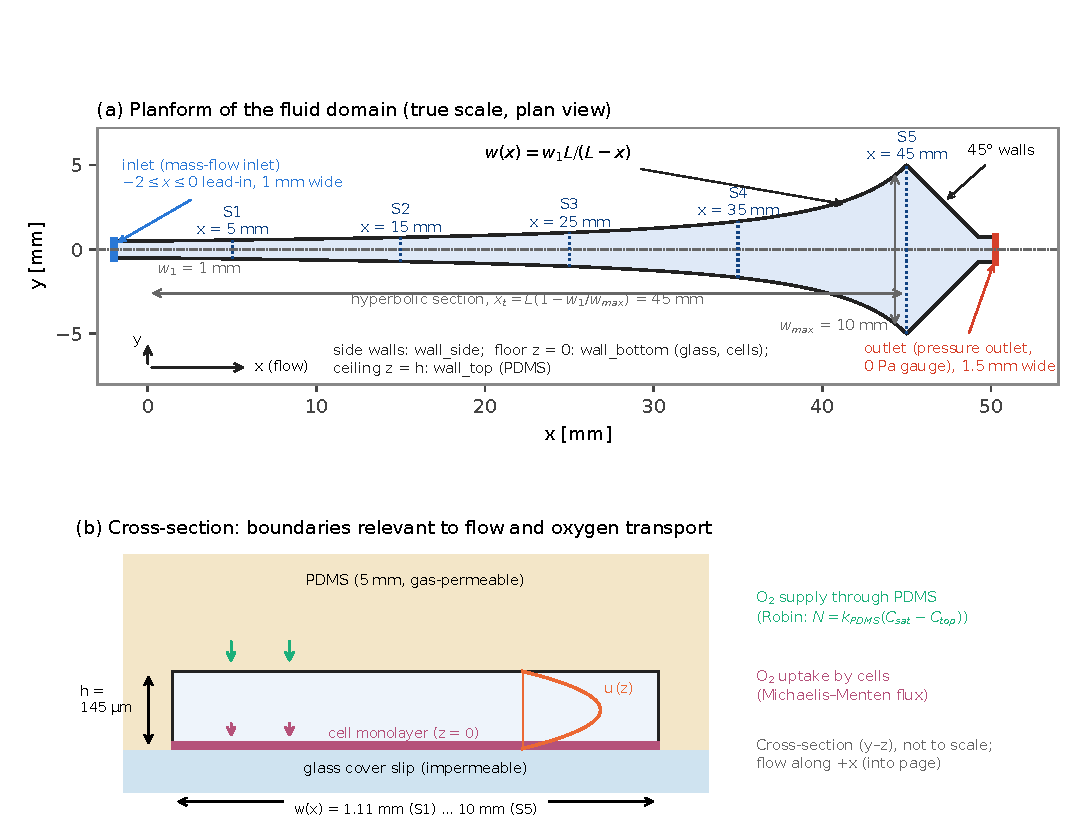
\includegraphics[width=\linewidth]{geometry_schematic.pdf}
\caption{Computational domain. (a) Planform at true scale, with the hyperbolic section, the \ang{45} converging walls, the boundaries and the five measurement stations S1--S5. (b) Schematic cross-section (not to scale). The cells sit on the glass floor ($z=0$, \texttt{wall\_bottom}); the lid and the side walls are PDMS. The oxygen fluxes drawn in (b) are used in Part B.}
\label{fig:geometry}
\end{figure}

\section{Coordinate system and boundaries}

The origin lies on the channel axis at the start of the hyperbolic section, on the floor. Here $x$ points downstream along the axis, $y$ across the width (so the side walls lie at $y=\pm w(x)/2$), and $z$ upwards across the gap ($0\le z\le h$). The mean flow is in the $+x$ direction. \Cref{tab:boundaries} lists the boundary surfaces. For the flow they are the inlet face, the outlet face and the no-slip walls. For oxygen it matters which wall is which: the cells occupy the glass floor, while the lid and the side walls are PDMS.

\begin{table}[htbp]
\centering
\caption{Boundary surfaces of the computational domain.}
\label{tab:boundaries}
\small
\begin{tabular}{@{}lll@{}}
\toprule
Surface & Location & Physical meaning\\
\midrule
\texttt{inlet} & $x=-\SI{2}{mm}$, $|y|\le\SI{0.5}{mm}$ & medium enters from the inlet port\\
\texttt{outlet} & $x=\SI{50.25}{mm}$, $|y|\le\SI{0.75}{mm}$ & medium leaves to the outlet port\\
\texttt{wall\_bottom} & $z=0$ & glass cover slip carrying the cell monolayer\\
\texttt{wall\_top} & $z=h$ & PDMS lid, \SI{5}{mm} thick\\
\texttt{wall\_side} & $y=\pm w(x)/2$ & PDMS side walls\\
\bottomrule
\end{tabular}
\end{table}

\section{Characteristic cross-sections}

\Cref{tab:stations} lists the local geometry at the stations. Two ratios control how well the analytical theory works. The first is the local aspect ratio $h/w$, which measures the influence of the side walls on the flow. It falls from 0.145 at the inlet to 0.0145 at S5. The second is the wall half-angle $\theta=\arctan[\tfrac12\,\dd w/\dd x]$, which measures how quickly the planform changes. Since
\begin{equation}
\frac{1}{2}\frac{\dd w}{\dd x}=\frac{w_1L}{2(L-x)^2},
\label{eq:geo_slope}
\end{equation}
the half-angle grows from \ang{0.57} at the inlet to \ang{6.3} at S4 and reaches \ang{45} at S5, where the diverging walls meet the converging ones. S5 is therefore not a ``slowly varying'' section. It is the corner of the planform, and this fact explains several results in \cref{ch:validation}.

\begin{table}[htbp]
\centering
\caption{Local geometry at the inlet of the hyperbolic section and at the stations ($h=\SI{145}{\micro\metre}$). $f$ is the rectangular-duct flux factor of \cref{eq:th_flux_factor}.}
\label{tab:stations}
\small
\begin{tabular}{@{}lcccccc@{}}
\toprule
Section & $x$ [mm] & $w$ [mm] & $h/w$ & $D_h$ [\si{\micro\metre}] & half-angle $\theta$ & $f(h/w)$\\
\midrule
inlet of hyperbola & 0 & 1.000 & 0.1450 & 253.3 & \ang{0.57} & 0.9086\\
S1 & 5 & 1.111 & 0.1305 & 256.5 & \ang{0.71} & 0.9178\\
S2 & 15 & 1.429 & 0.1015 & 263.3 & \ang{1.17} & 0.9360\\
S3 & 25 & 2.000 & 0.0725 & 270.4 & \ang{2.29} & 0.9543\\
S4 & 35 & 3.333 & 0.0435 & 277.9 & \ang{6.34} & 0.9726\\
S5 & 45 & 10.00 & 0.0145 & 285.9 & \ang{45} (corner) & 0.9909\\
\bottomrule
\end{tabular}
\end{table}

\section{Symmetry}

The planform is symmetric about the axis $y=0$. The flow problem is also symmetric about the mid-plane $z=h/2$, because the floor and the lid are both no-slip walls. A half or quarter model would therefore give the same flow field. The simulations nevertheless used the full domain, so the symmetry is a check on the results rather than a constraint: the shear on the floor and on the lid agrees to \SIrange{0.1}{0.8}{\percent} (\cref{sec:val_transverse}). For oxygen, the symmetry about the mid-plane is broken, because the cells consume oxygen at the floor while the lid may supply it. Only the symmetry about the axis remains.

\section{Why the dimensions matter}

The aspect ratio is small, $h/w\le0.145$, so the flow in each cross-section is close to the flow between two infinite plates. The velocity is parabolic in $z$ and almost uniform in $y$, except within about one gap height of each side wall. The shear on the floor then depends on the local width only, $\taw\propto1/w(x)$, and the hyperbolic width makes it linear in $x$. The height enters as $\taw\propto h^{-2}$ and $\Delta p\propto h^{-3}$. A \SI{3.4}{\percent} error in $h$ (\SI{145}{} instead of \SI{150}{\micro\metre}) therefore changes the shear by about \SI{7}{\percent} and the pressure drop by about \SI{11}{\percent}, which is why the height inconsistency of the reference paper matters. For oxygen, $h$ sets the diffusion time across the gap and $w(x)$ sets the area of cells fed by a given flow (\cref{ch:o2analytical}).

\chapter{Mathematical Formulation: Fluid Flow}
\label{ch:governing}

\section{Conservation of mass}

For a fluid of density $\rho$ and velocity $\vect u$, conservation of mass in a fixed control volume gives the continuity equation
\begin{equation}
\frac{\partial\rho}{\partial t}+\nabla\cdot(\rho\vect u)=0 .
\label{eq:gov_cont_general}
\end{equation}
The first term is the rate at which mass accumulates in a unit volume; the second is the net mass outflow per unit volume. The culture medium is a liquid. Pressure differences in the chip are below \SI{250}{Pa} and temperature is held at \SI{37}{\celsius}, so its density changes by a negligible fraction and $\rho$ is constant. \Cref{eq:gov_cont_general} then reduces to the incompressibility condition
\begin{equation}
\nabla\cdot\vect u=\frac{\partial u_x}{\partial x}+\frac{\partial u_y}{\partial y}+\frac{\partial u_z}{\partial z}=0 .
\label{eq:gov_cont}
\end{equation}
Physically, \cref{eq:gov_cont} says that the volumetric flow rate $Q$ through every cross-section of the channel is the same. This is what links the local velocity, and hence the shear, to the local width: as $w(x)$ grows, the same $Q$ is spread over a larger cross-section and the fluid slows down.

\section{Conservation of momentum}

Newton's second law for a fluid element of a Newtonian fluid with constant density and viscosity gives the Navier--Stokes equations \citep{BSL2002,Batchelor1967}:
\begin{equation}
\underbrace{\rho\left(\frac{\partial\vect u}{\partial t}+\vect u\cdot\nabla\vect u\right)}_{\text{inertia}}
=\underbrace{-\nabla p}_{\text{pressure force}}
+\underbrace{\mu\nabla^2\vect u}_{\text{viscous force}}
+\underbrace{\rho\vect g}_{\text{body force}} .
\label{eq:gov_ns}
\end{equation}
The left-hand side is the mass times the acceleration of a fluid element. It contains the local acceleration $\partial\vect u/\partial t$ and the convective acceleration $\vect u\cdot\nabla\vect u$, which appears when a fluid element moves into a region of different velocity, as it does here because the channel widens. On the right-hand side, $-\nabla p$ is the net pressure force per unit volume, $\mu\nabla^2\vect u$ is the net viscous force (the divergence of the Newtonian stress tensor $\mu[\nabla\vect u+(\nabla\vect u)^{\mathsf T}]$ when $\nabla\cdot\vect u=0$), and $\rho\vect g$ is gravity. The wall shear stress, the central quantity of this project, is the tangential viscous stress on the floor:
\begin{equation}
\taw=\mu\left.\frac{\partial u_x}{\partial z}\right|_{z=0}
\label{eq:gov_tauw}
\end{equation}
(strictly the magnitude of $\mu\,\partial\vect u_{\parallel}/\partial z$; on the axis only the $x$-component is non-zero).

For constant density, gravity can be absorbed into a modified pressure $P=p-\rho\vect g\cdot\vect r$. It then disappears from \cref{eq:gov_ns} and from the boundary conditions, because the chip has no free surface. The hydrostatic difference across the gap, $\rho gh\approx\SI{1.4}{Pa}$, is comparable to the axial pressure drop, but it does not drive any flow. The Fluent model has gravity switched off, so its pressure is the modified pressure $P$ (written $p$ from here on).

\section{Model assumptions and their verification}

\Cref{tab:assumptions} lists each assumption, the evidence for it in this project and its consequence. All of them hold for the simulations. Only one, the neglect of side walls, fails in the simplest analytical model (T1), and it is removed in T2 and T3 (\cref{ch:theory}).

\begin{table}[htbp]
\centering
\caption{Assumptions of the flow model, checked against the present set-up.}
\label{tab:assumptions}
\small
\begin{tabularx}{\linewidth}{@{}p{0.2\linewidth}X p{0.17\linewidth}@{}}
\toprule
Assumption & Evidence in this project & Status\\
\midrule
Steady flow & Constant mass-flow inlet; viscous diffusion time across the gap $h^2/\nu=\SI{0.022}{s}$ is tiny compared with any change in the boundary conditions & valid (simulations steady)\\
Incompressible, constant $\rho$ & Liquid; $\Delta p<\SI{250}{Pa}$; isothermal at \SI{37}{\celsius} & valid\\
Newtonian, constant $\mu$ & Wall shear rates $\taw/\mu\approx\SIrange{0.15}{600}{s^{-1}}$; medium with \SI{10}{\percent} serum treated as Newtonian with $\mu=\SI{0.94}{mPa.s}$ \tagP & assumed (not measured)\\
Laminar & $\Rey_{D_h}\le3.65$ (\cref{tab:dimensionless}) & valid\\
Gravity negligible & Absorbed in the modified pressure; no free surface & valid\\
No slip at walls & Liquid; molecular length scale $\sim\SI{0.3}{nm}$ gives $Kn\sim10^{-6}$ & valid\\
Continuum & As above & valid\\
Locally fully developed & Development length $(0.6+0.05\Rey_h)h\approx\SI{0.09}{mm}\ll\SI{2}{mm}$ lead-in; wall half-angle $\le\ang{6.3}$ up to S4 & valid for $x\lesssim\SI{40}{mm}$, not at S5\\
Side walls negligible & $h/w=0.13$ at S1 & \textbf{not valid} for T1; corrected in T2/T3\\
\bottomrule
\end{tabularx}
\end{table}

\section{Dimensionless numbers}
\label{sec:dimensionless}

\paragraph{Reynolds number.} The ratio of inertial to viscous forces, based on the hydraulic diameter at the inlet of the hyperbolic section ($D_h=\SI{0.253}{mm}$, $\bar U=Q/(w_1h)$), is
\begin{equation}
\Rey_{D_h}=\frac{\rho\bar UD_h}{\mu}=0.0067,\ 0.030\ \text{and}\ 3.65
\end{equation}
for 0.22, 1 and \SI{120}{\uLmin}. These values are far below the laminar--turbulent transition ($\sim2000$). In a thin gap the relevant comparison is the convective acceleration $\rho u_x\,\partial u_x/\partial x\sim\rho\bar U^2/\ell$, where $\ell=L-x$ is the length over which the width changes, against the viscous term $\mu\bar U/h^2$. Their ratio $\Rey_h\,h/\ell$ is the reduced Reynolds number of lubrication theory. Since $\ell\ge w$ for $x\lesssim\SI{43}{mm}$, it is bounded by the conservative estimate
\begin{equation}
\Rey^*=\frac{\rho\bar Uh}{\mu}\,\frac{h}{w}=\num{5.6e-4},\ \num{2.5e-3}\ \text{and}\ 0.30 ,
\label{eq:gov_restar}
\end{equation}
which is small at all three flow rates. Inertia is therefore negligible and the flow is a Stokes flow: velocity, pressure and shear must all scale exactly with $Q$. This is tested in \cref{sec:val_scaling}.

\paragraph{Aspect ratio.} The aspect ratio $h/w$ (\cref{tab:stations}) measures the share of the drag carried by the side walls. For $h/w\to0$ the flow is that between infinite plates. At $h/w=0.13$, the side walls carry enough drag to raise the floor shear on the axis by \SI{9}{\percent} (\cref{sec:th_sidewall}).

\paragraph{Hydraulic diameter.} $D_h=2wh/(w+h)$ ranges from \SI{253}{\micro\metre} to \SI{286}{\micro\metre} and approaches $2h$ as $w\gg h$. It is used only to quote a conventional Reynolds number. The physics of the thin gap is governed by $h$, not $D_h$.

\paragraph{P\'eclet and Damk\"ohler numbers.} These are relevant to oxygen transport and are introduced in \cref{ch:o2equations}.

\begin{table}[htbp]
\centering
\caption{Dimensionless numbers of the flow at the inlet of the hyperbolic section ($x=0$, $w=w_1$), where they are largest.}
\label{tab:dimensionless}
\small
\begin{tabular}{@{}lccc@{}}
\toprule
Quantity & \SI{0.22}{\uLmin} & \SI{1}{\uLmin} & \SI{120}{\uLmin}\\
\midrule
Mean velocity $\bar U$ [\si{mm/s}] & 0.0253 & 0.115 & 13.8\\
$\Rey_{D_h}=\rho\bar UD_h/\mu$ & 0.0067 & 0.030 & 3.65\\
$\Rey_h=\rho\bar Uh/\mu$ & 0.0038 & 0.017 & 2.09\\
$\Rey^*=\Rey_h\,h/w$ & \num{5.6e-4} & \num{2.5e-3} & 0.30\\
Development length $(0.6+0.05\Rey_h)h$ [mm] & 0.087 & 0.087 & 0.102\\
Viscous time $h^2/\nu$ [s] & 0.022 & 0.022 & 0.022\\
\bottomrule
\end{tabular}
\end{table}

\chapter{Theoretical Flow Model and Analytical Predictions}
\label{ch:theory}

The full Navier--Stokes equations have no closed-form solution in the widening channel. The geometry is, however, thin and slowly varying, which is exactly the situation that lubrication (Hele-Shaw) theory is designed for \citep{Batchelor1967,Bruus2008}. This chapter derives that theory step by step. It is developed at three levels:
\begin{itemize}
\item T1 is the parallel-plate result used by Delon \emph{et al.} (their Eq.~2);
\item T2 corrects T1 for the drag of the side walls, using the exact solution for a rectangular duct;
\item T3 keeps the two-dimensional character of the planform, which matters near the outlet corner.
\end{itemize}
Each level removes one assumption of the previous one, so comparing them with the CFD shows which physical effect causes which deviation.

\section{Lubrication scaling}
\label{sec:th_scaling}

Let the channel have height $h$, local width $w$ and an axial length scale $\ell=w/|\dd w/\dd x|$ over which the width changes. From \cref{eq:intro_width}, $\ell=L-x$, which is \SI{50}{mm} at the inlet and \SI{15}{mm} at S4. With $\bar U$ the mean velocity, the terms of the $x$-momentum equation scale as
\begin{equation}
\underbrace{\rho u_x\frac{\partial u_x}{\partial x}}_{\rho\bar U^2/\ell}
=-\frac{\partial p}{\partial x}
+\mu\Big(\underbrace{\frac{\partial^2u_x}{\partial x^2}}_{\bar U/\ell^2}
+\underbrace{\frac{\partial^2u_x}{\partial y^2}}_{\bar U/w^2}
+\underbrace{\frac{\partial^2u_x}{\partial z^2}}_{\bar U/h^2}\Big).
\label{eq:th_scaling}
\end{equation}
Relative to the dominant viscous term $\mu\bar U/h^2$, the other terms are of the following order:
\begin{itemize}
\item axial viscous diffusion, $(h/\ell)^2\le10^{-4}$ up to S4;
\item transverse viscous diffusion, $(h/w)^2\le0.02$, except within a distance of order $h$ from a side wall;
\item inertia, $\Rey_h\,h/\ell$. This is smaller than the conservative estimate $\Rey^*=\Rey_h\,h/w$ of \cref{tab:dimensionless} wherever $\ell\ge w$ (i.e.\ for $x\lesssim\SI{43}{mm}$), so it is at most 0.3 and below $3\times10^{-3}$ at the two cell-culture flow rates.
\end{itemize}
Continuity gives $u_z\sim\bar Uh/\ell$. The $z$-momentum equation then shows that $\partial p/\partial z$ is smaller than $\partial p/\partial x$ by a factor $(h/\ell)^2$, so the pressure is uniform across the gap: $p=p(x,y)$. To leading order, the momentum equations reduce to
\begin{equation}
\frac{\partial p}{\partial x}=\mu\frac{\partial^2u_x}{\partial z^2},\qquad
\frac{\partial p}{\partial y}=\mu\frac{\partial^2u_y}{\partial z^2},\qquad
\frac{\partial p}{\partial z}=0 .
\label{eq:th_lub}
\end{equation}
Physically, every vertical column of fluid is in local equilibrium between the pressure gradient and the viscous drag of the floor and the lid. Inertia and the slow change of the planform do not enter.

\section{Local velocity profile}

Because $p$ does not depend on $z$, the first equation of \cref{eq:th_lub} can be integrated twice in $z$:
\begin{align}
\frac{\partial^2u_x}{\partial z^2}&=\frac{1}{\mu}\frac{\partial p}{\partial x}
\;\Rightarrow\;
u_x=\frac{1}{2\mu}\frac{\partial p}{\partial x}z^2+c_1z+c_2 .
\end{align}
No slip on the floor and the lid, $u_x(z=0)=u_x(z=h)=0$, gives $c_2=0$ and $c_1=-\frac{h}{2\mu}\frac{\partial p}{\partial x}$. Hence
\begin{equation}
u_x(x,y,z)=-\frac{1}{2\mu}\frac{\partial p}{\partial x}\,z\,(h-z),
\qquad
u_y(x,y,z)=-\frac{1}{2\mu}\frac{\partial p}{\partial y}\,z\,(h-z).
\label{eq:th_parabola}
\end{equation}
The profile across the gap is a parabola, with its maximum at mid-height,
\begin{equation}
u_{\max}=-\frac{h^2}{8\mu}\frac{\partial p}{\partial x}=\frac32\bar U .
\label{eq:th_umax}
\end{equation}
\Cref{eq:th_umax} links the peak velocity rigidly to the local pressure gradient, and we use it in \cref{sec:val_offset} to test the internal consistency of the CFD.

\section{Depth-averaged flux and the Hele-Shaw equation}

Integrating \cref{eq:th_parabola} across the gap gives the flux per unit width, $\vect q=\int_0^h(u_x,u_y)\,\dd z$:
\begin{equation}
\vect q=-\frac{h^3}{12\mu}\nabla p ,
\qquad \nabla=\left(\frac{\partial}{\partial x},\frac{\partial}{\partial y}\right).
\label{eq:th_darcy}
\end{equation}
This has the form of Darcy's law, with permeability $h^3/12\mu$. Integrating the continuity equation \cref{eq:gov_cont} over the gap, using $u_z=0$ at $z=0$ and $z=h$, gives $\nabla\cdot\vect q=0$. For a constant height this becomes
\begin{equation}
\nabla\cdot\left(\frac{h^3}{12\mu}\nabla p\right)=0
\quad\Longrightarrow\quad
\frac{\partial^2p}{\partial x^2}+\frac{\partial^2p}{\partial y^2}=0 .
\label{eq:th_laplace}
\end{equation}
Within the lubrication approximation the pressure is a harmonic function of the planform coordinates. The side walls carry the condition of zero normal flux, $\partial p/\partial n=0$. This two-dimensional problem is the basis of model T3 (\cref{sec:th_T3}).

\section{One-dimensional solution for the hyperbolic channel (T1)}

If the planform changes slowly, the iso-bars are straight lines across the width, so $p=p(x)$ and $u_y\approx0$. Ignoring the side walls (infinite plates of width $w$), the total flow rate is $Q=w(x)\,q_x$. From \cref{eq:th_darcy},
\begin{equation}
Q=-\frac{w(x)h^3}{12\mu}\frac{\dd p}{\dd x}
\quad\Longrightarrow\quad
\frac{\dd p}{\dd x}=-\frac{12\mu Q}{h^3w(x)} .
\label{eq:th_dpdx_general}
\end{equation}
\paragraph{Pressure gradient.} Substituting the hyperbolic width $w(x)=w_1L/(L-x)$,
\begin{equation}
\frac{\dd p}{\dd x}=-\frac{12\mu Q}{h^3w_1}\left(1-\frac{x}{L}\right).
\label{eq:th_dpdx}
\end{equation}
The pressure gradient therefore falls \emph{linearly} along the axis. The hyperbolic width was chosen precisely so that $1/w(x)$ is linear in $x$.

\paragraph{Pressure distribution.} Integrating \cref{eq:th_dpdx} from 0 to $x$,
\begin{equation}
p(0)-p(x)=\frac{12\mu Q}{h^3w_1}\left(x-\frac{x^2}{2L}\right),
\label{eq:th_p}
\end{equation}
a parabola that is concave downwards and flattens towards the outlet. Over the whole hyperbolic section the pressure drop is
\begin{equation}
\Delta p_{0\to x_t}=\frac{12\mu Q}{h^3w_1}\left(x_t-\frac{x_t^2}{2L}\right)
\equiv R_{\mathrm{hyd}}\,Q,
\qquad R_{\mathrm{hyd}}=\SI{9.16e10}{Pa.s/m^3}.
\label{eq:th_dp}
\end{equation}
With $Q=\SI{0.9998}{\uLmin}$ this gives $\Delta p_{0\to45}=\SI{1.526}{Pa}$ \tagT.

\paragraph{Wall shear stress.} The floor shear follows from \cref{eq:gov_tauw,eq:th_parabola}:
\begin{equation}
\taw=\mu\left.\frac{\partial u_x}{\partial z}\right|_{z=0}=-\frac{h}{2}\frac{\dd p}{\dd x}
=\frac{6\mu Q}{h^2w_1}\left(1-\frac{x}{L}\right)
=\frac{6\mu\bar U}{h}=\frac{4\mu u_{\max}}{h}.
\label{eq:th_tauw}
\end{equation}
This is Eq.~2 of Delon \emph{et al.} (\cref{eq:lit_eq2}). The shear falls linearly from $\tau_1=6\mu Q/(h^2w_1)$ at $x=0$ to $\tau_1/10$ at $x_t$; the ratio is fixed by $w_{\max}/w_1=10$. For \SI{1}{\uLmin}, $\tau_1=\SI{4.47e-3}{Pa}=\SI{0.0447}{\dyncm}$, and for \SI{0.22}{\uLmin}, $\tau_1=\SI{9.84e-4}{Pa}$ \tagT. The identity $\taw=(h/2)|\dd p/\dd x|$ is a momentum balance on a slab of fluid between the floor and the mid-plane. It holds for any locally parabolic flow, whatever the planform, and it is used in \cref{sec:val_cross} to check the CFD.

\paragraph{Shear above the floor.} The viscous shear stress varies linearly across the gap, $\tau(z)=\taw(1-2z/h)$. At $z=\SI{20}{\micro\metre}$, which the reference paper uses as the height of the cell monolayer, $\tau=0.724\,\taw$. The paper's estimate $\tau_{\mathrm{cell}}=3\taw$ \citep{GaverKute1998} instead accounts for the disturbance of the flow by the cell itself, and is not tested here.

\paragraph{Validity of T1.} T1 requires $h/w\ll1$ (no side-wall drag), $\dd w/\dd x\ll1$ (straight iso-bars) and $\Rey^*\ll1$, and it applies only to $0\le x\le x_t$.

\section{Side-wall correction: exact rectangular-duct solution (T2)}
\label{sec:th_sidewall}

T1 treats the channel as infinitely wide, but at the inlet $h/w=0.145$. To quantify the side-wall effect, consider fully developed flow in a rectangle $-w/2\le y\le w/2$, $0\le z\le h$, driven by a constant gradient $G=-\dd p/\dd x$. Keeping the transverse viscous term,
\begin{equation}
\frac{\partial^2u_x}{\partial y^2}+\frac{\partial^2u_x}{\partial z^2}=-\frac{G}{\mu},
\qquad u_x=0\ \text{on all four walls.}
\label{eq:th_poisson}
\end{equation}
\paragraph{Solution.} Write $u_x=u_{pp}(z)+u_h(y,z)$, where $u_{pp}=\frac{G}{2\mu}z(h-z)$ is the parallel-plate solution. The correction $u_h$ satisfies Laplace's equation, vanishes at $z=0$ and $z=h$, and must cancel $u_{pp}$ on the side walls. Expanding $z(h-z)$ in a sine series on $[0,h]$,
\begin{equation}
z(h-z)=\sum_{n\ \mathrm{odd}}\frac{8h^2}{\pi^3n^3}\sin\frac{n\pi z}{h},
\end{equation}
and seeking $u_h=\sum_nB_n\sin(n\pi z/h)\cosh(n\pi y/h)$, which is harmonic and even in $y$, the condition $u_h(\pm w/2,z)=-u_{pp}(z)$ fixes $B_n$. Hence
\begin{equation}
u_x(y,z)=\frac{G}{2\mu}\left[z(h-z)-\sum_{n\ \mathrm{odd}}\frac{8h^2}{\pi^3n^3}\sin\frac{n\pi z}{h}\,\frac{\cosh(n\pi y/h)}{\cosh(n\pi w/2h)}\right].
\label{eq:th_rect_u}
\end{equation}
\paragraph{Flux factor.} Integrating \cref{eq:th_rect_u} over the section gives $Q=\frac{Gwh^3}{12\mu}f(h/w)$, with
\begin{equation}
f\!\left(\frac hw\right)=1-\frac{192}{\pi^5}\frac{h}{w}\sum_{n\ \mathrm{odd}}\frac{1}{n^5}\tanh\frac{n\pi w}{2h}\;\approx\;1-0.630\,\frac hw\quad(w\gg h).
\label{eq:th_flux_factor}
\end{equation}
The side walls reduce the flux at a given gradient. Conversely, at a given flow rate they raise the pressure gradient by $1/f$. With $h/w$ evaluated locally, T2 is
\begin{equation}
\left.\frac{\dd p}{\dd x}\right|_{T2}=\frac{1}{f(h/w(x))}\left.\frac{\dd p}{\dd x}\right|_{T1},
\qquad
\taw^{T2}(y=0)=\frac{\taw^{T1}}{f(h/w(x))}.
\label{eq:th_T2}
\end{equation}
The correction factor $1/f$ is 1.090 at S1, 1.068 at S2, 1.048 at S3, 1.028 at S4 and 1.009 at S5 (\cref{tab:stations}). T2 thus predicts that the CFD shear on the axis should exceed Eq.~2 by about $0.63\,h/w$, most strongly near the inlet.

\paragraph{Transverse distribution of the floor shear.} Differentiating \cref{eq:th_rect_u} at $z=0$,
\begin{equation}
\frac{\tau(y)}{\tau(0)}=\frac{S(y)}{S(0)},\qquad
S(y)=1-\sum_{n\ \mathrm{odd}}\frac{8}{\pi^2n^2}\,\frac{\cosh(n\pi y/h)}{\cosh(n\pi w/2h)} .
\label{eq:th_tau_y}
\end{equation}
Near a side wall, at a distance $\delta=w/2-|y|$ from it, the $n=1$ term dominates. There $\cosh(\pi y/h)/\cosh(\pi w/2h)\approx e^{-\pi\delta/h}$, so that
\begin{equation}
\frac{\tau}{\tau(0)}\approx1-\frac{8}{\pi^2}e^{-\pi\delta/h}.
\end{equation}
The shear is more than a fraction $\varepsilon$ below its core value within the side-wall layer
\begin{equation}
\delta_\varepsilon=\frac{h}{\pi}\ln\frac{8}{\pi^2\varepsilon}
=\SI{0.129}{mm}\ (\varepsilon=\SI{5}{\percent}),\quad
\SI{0.171}{mm}\ (\SI{2}{\percent}),\quad
\SI{0.097}{mm}\ (\SI{10}{\percent}).
\label{eq:th_delta}
\end{equation}
The layer thickness scales with the gap $h$ and is independent of the width. The half-width of the uniform-shear band is therefore $d(\varepsilon)=w/2-\delta_\varepsilon$, and the uniform fraction $2d/w$ must grow as the channel widens. This is the theoretical basis for the imaging zones of Delon \emph{et al.}, and it is tested in \cref{sec:val_transverse}.

\section{Two-dimensional Hele-Shaw model of the full planform (T3)}
\label{sec:th_T3}

T1 and T2 assume straight iso-bars. Near $x=x_t$, however, the wall half-angle jumps from \ang{45} diverging to \ang{45} converging. The flow must turn towards the outlet within a distance comparable to the width (\SI{10}{mm}): the corners become low-velocity regions and the flow along the axis accelerates. To capture this, the depth-averaged equation \cref{eq:th_laplace} was solved on the full planform. The side-wall correction was included in the permeability:
\begin{equation}
\nabla\cdot\left[K(x)\nabla p\right]=0,\qquad K=\frac{h^3f(h/w(x))}{12\mu},
\label{eq:th_T3}
\end{equation}
with these boundary conditions:
\begin{itemize}
\item zero normal flux on the side walls;
\item a uniform inflow giving $Q$ at the inlet of the lead-in;
\item $p=0$ at the outlet.
\end{itemize}
The domain (half planform, symmetry at $y=0$) includes the lead-in, the hyperbola, the \ang{45} walls and the outlet duct. It was discretised with linear finite elements, with \SI{20}{\micro\metre} axial spacing and 81 nodes across the half-width (\cref{app:repro}). The floor shear on the axis is $(h/2)|\nabla p|$ and the mid-plane velocity is $h\tau/(4\mu)$. In the straight lead-in, T3 reproduces the exact rectangular-duct gradient to a relative error of $10^{-5}$. In the slowly varying part of the hyperbola it reduces to T2. It does not resolve the side-wall layer itself, because that is a three-dimensional feature of thickness $\sim h$. \Cref{fig:T3} shows the T3 shear field and its prediction that the axial shear departs from Eq.~2 from $x\approx\SI{40}{mm}$ onwards. The minimum is at $x=\SI{44.1}{mm}$, and at S5 the shear is \SI{54}{\percent} above Eq.~2 \tagT.

\begin{figure}[htbp]
\centering
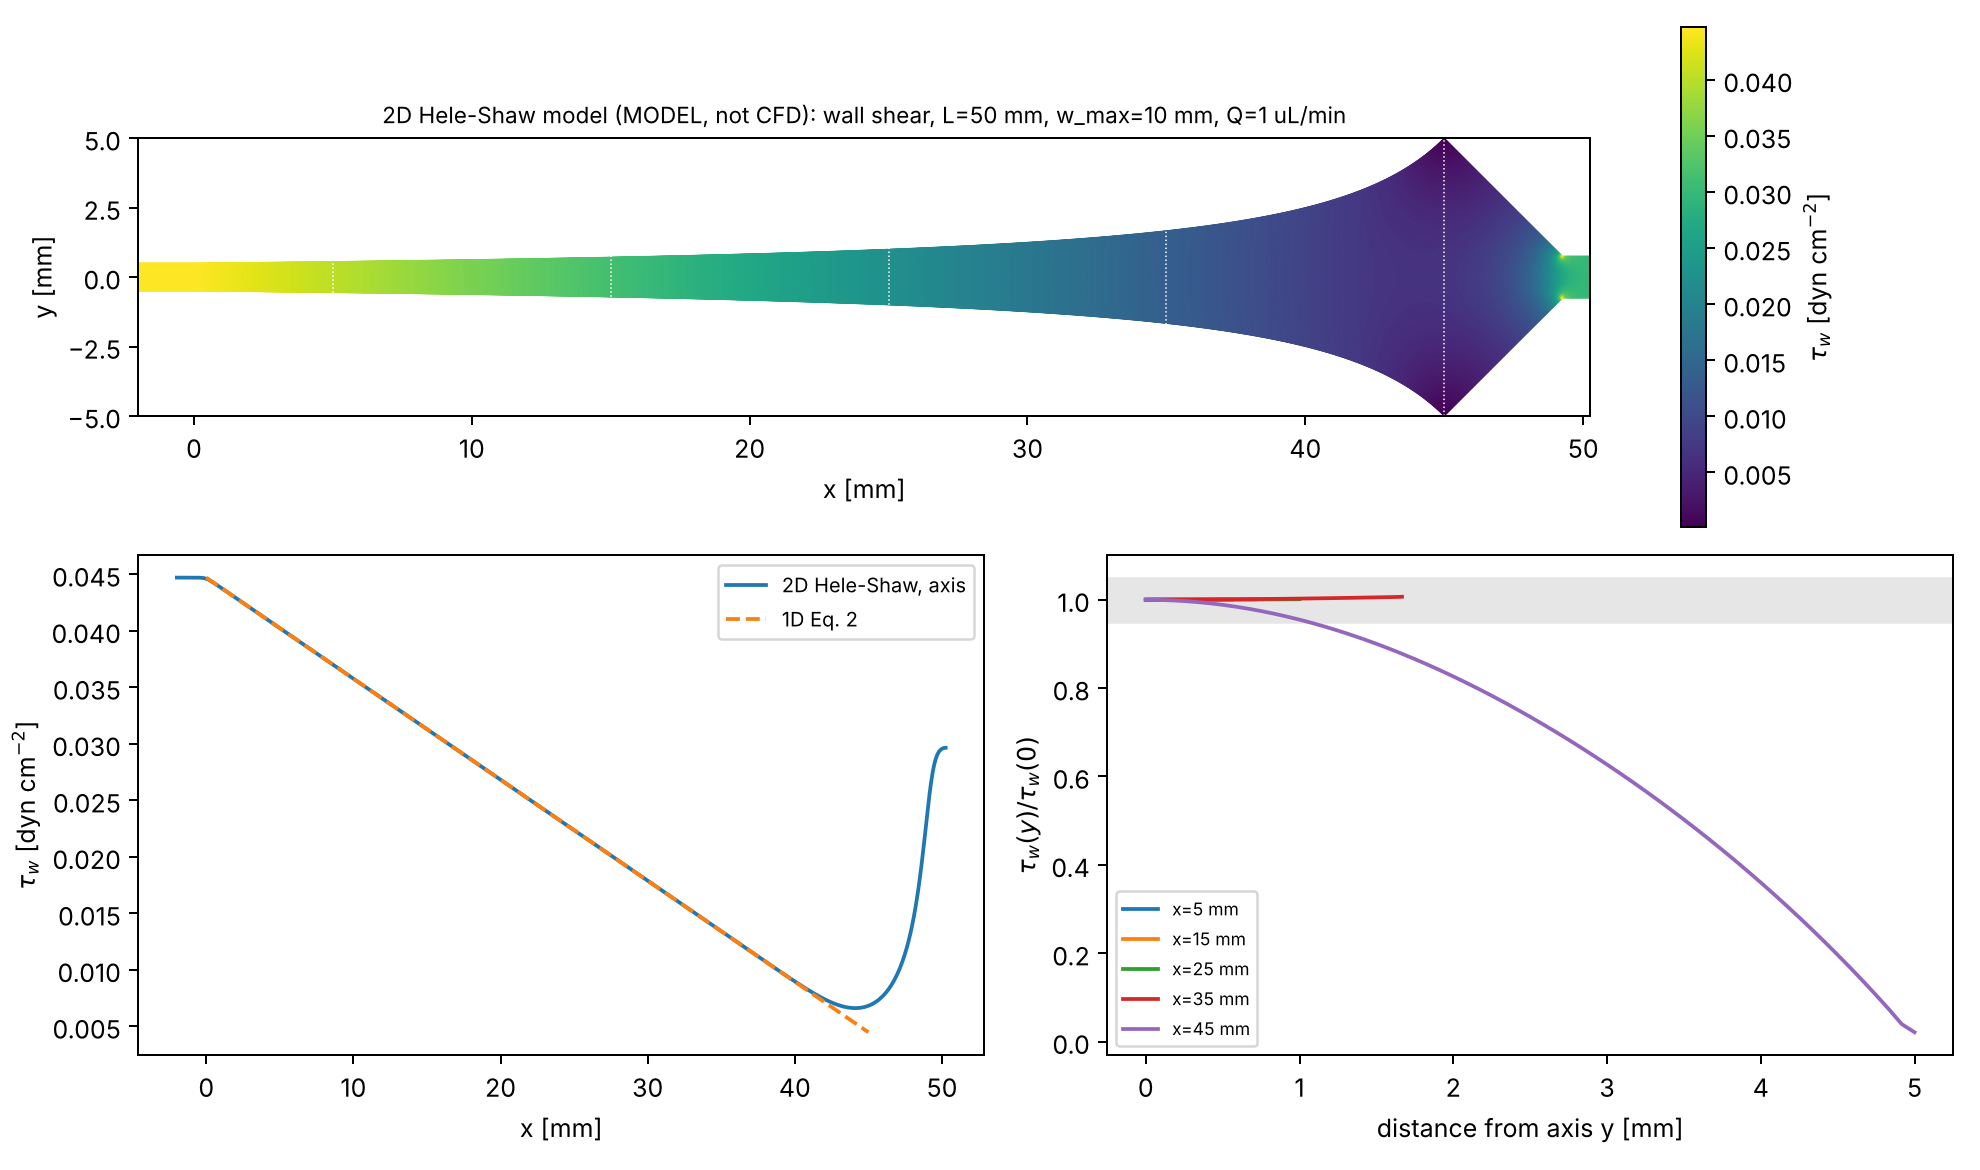
\includegraphics[width=0.95\linewidth]{T3_hs2d_W10_Q1.png}
\caption{Model T3, the two-dimensional Hele-Shaw solution at \SI{1}{\uLmin} \tagT. Top: wall shear on the floor over the planform (\si{\dyncm}). Bottom left: axial shear compared with Eq.~2; the two coincide until $x\approx\SI{40}{mm}$, after which the converging outlet raises the shear. Bottom right: transverse shear profiles normalised by the axis value. They are flat at S1--S4 (T3 has no side-wall layer) and dome-shaped at S5.}
\label{fig:T3}
\end{figure}

\section{Summary of analytical predictions}

\Cref{tab:theory_stations} collects the predictions at the five stations for \SI{1}{\uLmin} ($Q=\SI{0.9998}{\uLmin}$). All quantities are proportional to $Q$. These are the quantities compared with the CFD in \cref{ch:validation}:
\begin{itemize}
\item the axial pressure $p(x)$, the pressure drop and the gradient $\dd p/\dd x$;
\item the centre-line wall shear $\taw(x)$ and its ratio to Eq.~2;
\item the transverse shear profile $\tau(y)/\tau(0)$ and the uniform half-width $d(\varepsilon)$;
\item the mid-plane velocity and the momentum balance $\taw=(h/2)|\dd p/\dd x|$.
\end{itemize}
The parabolic profile $u_x(z)$ of \cref{eq:th_parabola} could not be compared, because the velocity exports contain no $z$ coordinate (\cref{sec:num_exports}).

\begin{table}[htbp]
\centering
\caption{Analytical predictions at the stations, $Q=\SI{0.9998}{\uLmin}$ \tagT. Shear in mPa (\SI{1}{mPa}=\SI{0.01}{\dyncm}). The mid-plane velocity and $d$ at S1--S4 are from T2; at S5 they are from T3.}
\label{tab:theory_stations}
\small
\begin{tabular}{@{}lccccccc@{}}
\toprule
Station & $\taw^{T1}$ & $\taw^{T2}$ & $\taw^{T3}$ & $-\dd p/\dd x|_{T1}$ & $-\dd p/\dd x|_{T2}$ & $u_{\mathrm{mid}}(0)$ & $d$ (\SI{\pm5}{\percent})\\
 & [mPa] & [mPa] & [mPa] & [Pa/m] & [Pa/m] & [mm/s] & [mm]\\
\midrule
S1 & 4.023 & 4.383 & 4.383 & 55.49 & 60.46 & 0.1690 & 0.427\\
S2 & 3.129 & 3.343 & 3.342 & 43.16 & 46.11 & 0.1289 & 0.586\\
S3 & 2.235 & 2.342 & 2.342 & 30.83 & 32.30 & 0.0903 & 0.871\\
S4 & 1.341 & 1.379 & 1.379 & 18.50 & 19.02 & 0.0532 & 1.538\\
S5 & 0.447 & 0.451 & 0.688 & 6.17 & 6.22 & 0.0265 & 1.050\\
\bottomrule
\end{tabular}
\end{table}

\chapter{Numerical Methodology and CFD Simulations}
\label{ch:numerics}

This chapter documents the simulations as they were run. Settings were taken from the Fluent report files that came with the results (\texttt{report.xml}) and from screenshots of the solver set-up. Where a setting is not documented, this is stated rather than assumed.

\section{Computational set-up}

\paragraph{Geometry preparation.} The planform of \cref{fig:geometry} was generated by a Python script (CadQuery) and exported as a STEP solid of height \SI{145}{\micro\metre}. The hyperbolic walls are single splines through 241 points, not polylines, which avoids the many small faces that polyline imports produce. The ports of the physical chip (3 and \SI{1.5}{mm} punched holes) were not modelled. Inflow enters through the face of the lead-in and outflow leaves through the face of the outlet duct. Named selections (\texttt{inlet}, \texttt{outlet}, walls) were defined before meshing.

\paragraph{Computational domain.} The domain is the full three-dimensional fluid volume (\SI{20.745}{\milli\metre\cubed}), without symmetry planes. The PDMS and the glass were not meshed; they enter the flow problem only as no-slip walls.

\paragraph{Mesh.} The mesh files and the mesh statistics were not included in the results we received, so the element type, the cell count and the quality metrics are not documented (\cref{app:missing}). Two properties can be inferred from the exported data:
\begin{enumerate}
\item \emph{Resolution across the gap.} In each cross-section the interior nodes carry four distinct velocity values, each appearing twice, for example 0.046, 0.091, 0.130 and \SI{0.160}{mm/s} per \ulmin\ at S1. This is the signature of eight interior node levels placed symmetrically about the mid-plane, i.e.\ about \textbf{nine cell layers across the \SI{145}{\micro\metre} gap}, slightly graded towards the walls.
\item \emph{Resolution near the side walls.} Wall nodes are \SIrange{0.08}{0.10}{mm} apart next to the side walls (\cref{tab:transverse_nodes}). This is comparable to the theoretical side-wall layer of \SI{0.129}{mm}, so the layer is only marginally resolved.
\end{enumerate}
No mesh images are available. The flow-rate cases used the same mesh: the number of nodes in every exported cross-section is identical in all three cases.

\paragraph{Mesh independence.} Only one mesh was run, so mesh independence could not be demonstrated. A study has been designed (\cref{sec:num_gci}) but not yet carried out. This is the most important open point of the validation (\cref{sec:val_offset}).

\section{Solver set-up}
\label{sec:num_solver}

\Cref{tab:solver} lists the solver settings.

\begin{table}[htbp]
\centering
\caption{ANSYS Fluent settings of the present simulations \tagC, from \texttt{report.xml} unless stated.}
\label{tab:solver}
\small
\begin{tabularx}{\linewidth}{@{}p{0.3\linewidth}X@{}}
\toprule
Setting & Value\\
\midrule
Software & ANSYS Fluent 2024 R1 (24.1.0), 3D, double precision\\
Formulation & Pressure-based, \textbf{steady}\\
Viscous model & Laminar; energy equation off (isothermal)\\
Material & Constant $\rho=\SI{981.8}{kg/m^3}$, $\mu=\SI{0.00094}{Pa.s}$ (medium at \SI{37}{\celsius} \citep{Delon2020})\\
Pressure--velocity coupling & SIMPLEC\\
Spatial discretisation & Pressure: PRESTO!; momentum: second-order upwind\\
Gradient method & Not contained in the exported report (Fluent default: least-squares cell-based)\\
Under-relaxation & Pressure 0.3, momentum 0.7\\
Gravity & Off (modified pressure, \cref{ch:governing})\\
Initialisation & Not documented\\
Convergence control & See \cref{sec:num_convergence}\\
\bottomrule
\end{tabularx}
\end{table}

Two choices differ from the reference paper. First, the paper ran a transient simulation with a time step of \SI{e-7}{s} to observe how the flow develops. Here a steady formulation was used, because the boundary conditions are constant, the viscous adjustment time is \SI{0.022}{s}, and only the steady state is analysed in both studies. Second, SIMPLEC replaces SIMPLE; both converge to the same steady solution, SIMPLEC usually in fewer iterations \citep{Patankar1980,Fluent2024}. PRESTO! interpolates pressure at the faces using a staggered-type stencil, which suits the strong pressure gradients normal to thin layers. Second-order upwind reduces numerical diffusion. At these Reynolds numbers convection is negligible in any case, so the choice of convection scheme has almost no effect on the flow.

\section{Convergence monitoring}
\label{sec:num_convergence}

The first runs used Fluent's \emph{absolute} residual criteria of $10^{-6}$ for continuity and the three momentum equations (\cref{fig:residuals}a), and the solver reported convergence after three iterations, with residuals printed as zero (\cref{fig:residuals}c; that console run also had the energy equation listed, so it predates the final set-up). This is not a meaningful convergence. At a mass flow of \SI{3.6e-9}{kg/s}, all fluxes in the domain are tiny, so the residuals start below an absolute threshold that was designed for flows of order \si{kg/s}. The settings were then changed (\cref{fig:residuals}b): the convergence criterion was set to \emph{none}, normalised and scaled residuals were plotted, and the solution was iterated until monitored physical quantities stopped changing.

\begin{figure}[htbp]
\centering
\begin{subfigure}[t]{0.47\linewidth}\centering
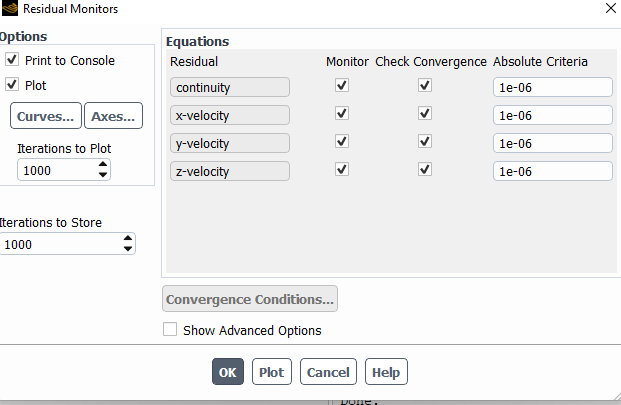
\includegraphics[width=\linewidth]{fluent_residuals_absolute.png}
\caption{Initial: absolute criteria $10^{-6}$.}
\end{subfigure}\hfill
\begin{subfigure}[t]{0.5\linewidth}\centering
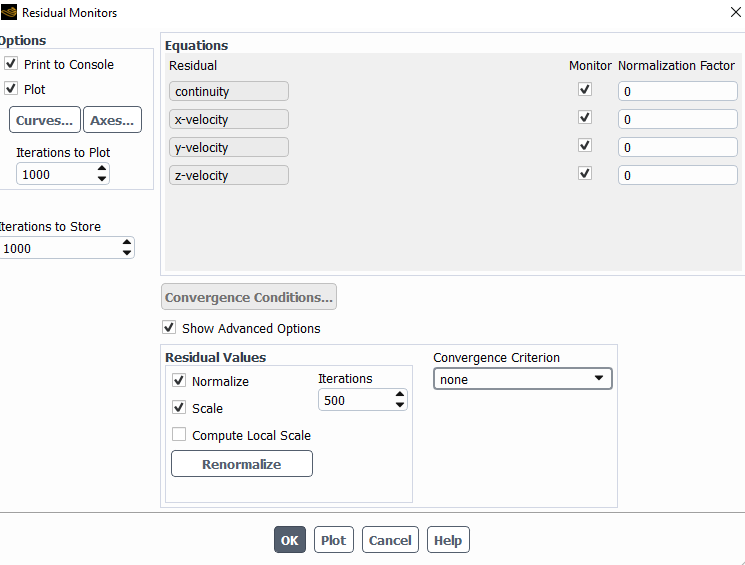
\includegraphics[width=\linewidth]{fluent_residuals_none.png}
\caption{Revised: criterion ``none'', normalised and scaled.}
\end{subfigure}

\vspace{2mm}
\begin{subfigure}[t]{0.75\linewidth}\centering
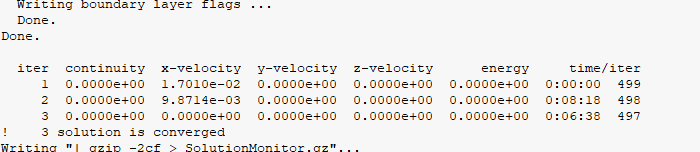
\includegraphics[width=\linewidth]{fluent_console_3iter.png}
\caption{Console message obtained with the initial settings.}
\end{subfigure}
\caption{Residual-monitor settings used during the project (screenshots from Fluent). With absolute criteria the very small fluxes of a \si{\micro\litre\per\minute} flow satisfied the criterion after three iterations. The revised settings rely on monitored quantities instead.}
\label{fig:residuals}
\end{figure}

The documents we received do not show which of the two settings produced the exported results, and they contain no residual history and no mass-flux report. Convergence therefore has to be judged from the results themselves. Four observations indicate a converged solution:
\begin{enumerate}
\item the pressure decreases monotonically at all 730 axial positions, in all three cases;
\item the wall shear and the pressure gradient obey the momentum balance $\taw=(h/2)|\dd p/\dd x|$ to within \SI{0.8}{\percent} (\cref{tab:momentum});
\item the three flow rates, which span a factor of 545, give results proportional to $Q$ to within \SI{0.08}{\percent} (\cref{sec:val_scaling}); solutions stopped at different stages of convergence would be unlikely to agree this closely;
\item the floor and lid shear agree to \SIrange{0.1}{0.8}{\percent}, as the mid-plane symmetry requires.
\end{enumerate}
The inlet/outlet mass balance (\emph{Reports $\to$ Fluxes}) should still be reported, because it is the only direct test of mass conservation.

\section{Boundary conditions}

\begin{table}[htbp]
\centering
\caption{Boundary conditions of the flow simulations \tagC.}
\label{tab:bc}
\small
\begin{tabularx}{\linewidth}{@{}p{0.1\linewidth}p{0.14\linewidth}p{0.26\linewidth}X@{}}
\toprule
Boundary & Fluent type & Value & Physical reasoning\\
\midrule
\texttt{inlet} & mass-flow inlet & $\dot m=\num{3.6e-9}$, \num{1.636e-8}, \SI{1.964e-6}{kg/s} (normal to face) & A syringe pump imposes the flow rate; $Q=\dot m/\rho=0.2200$, 0.9998, \SI{120.02}{\uLmin}. The face receives a uniform velocity, which develops into the duct profile within \SI{0.09}{mm}, far upstream of $x=0$.\\
\texttt{outlet} & pressure outlet & \SI{0}{Pa} gauge & Outlet port open to the reservoir at atmospheric pressure; only pressure differences matter in incompressible flow.\\
all walls & stationary wall & no slip, $\vect u=\vect 0$ & Continuum liquid on solid walls ($Kn\sim10^{-6}$).\\
\bottomrule
\end{tabularx}
\end{table}

The turbulence intensity and hydraulic diameter that Fluent requests at inlets and outlets are irrelevant for a laminar model and were left at their defaults. The uniform inlet velocity creates a local shear peak at the inlet face of the lead-in, which dominates the colour scale of the wall-shear contours (\cref{fig:contours}). Because the lead-in is \SI{2}{mm} long, more than 20 development lengths, this peak does not affect the hyperbolic section.

\section{Exported data}
\label{sec:num_exports}

For each flow rate, twelve Fluent XY exports were analysed:
\begin{itemize}
\item static pressure and wall shear stress along the axis ($0\le x\le\SI{50.25}{mm}$, 740 points on a wall at $y=0$);
\item wall shear stress at the five stations, on the plane $x=$ const, against $y$;
\item velocity magnitude at the five stations, on the plane $x=$ const, against $y$.
\end{itemize}
Two features of these exports constrain the analysis:
\begin{enumerate}
\item The cross-section exports contain the nodes of a whole plane plotted against $y$, at all heights, without the $z$ coordinate. Wall shear is non-zero only at the wall nodes, and these come in near-coincident floor/lid pairs. The velocity is the magnitude $|\vect u|$, not $u_x$. The parabolic profile $u_x(z)$ therefore cannot be reconstructed.
\item The axial line lies on a wall at $y=0$. Whether it is the floor or the lid cannot be told from the data, but by symmetry the two agree to within \SI{0.8}{\percent}.
\end{enumerate}
The raw files were parsed from their headers and kept unchanged. Duplicated positions were averaged only for interpolation and differentiation. Local pressure gradients were obtained by least-squares regression over a $\pm\SI{0.4}{mm}$ window, and station values by linear interpolation. The post-processing scripts are listed in \cref{app:repro}.

\section{Numerical reliability}

\paragraph{What has been established.} Iterative convergence is supported by the internal consistency checks listed above. Mass conservation in the integral sense is supported by the exact scaling with $Q$, but it has not been checked directly. The simulations are numerically stable: they show no oscillation, no backflow and no non-monotonic pressure.

\paragraph{What has not been established.} The magnitude of the discretisation error is unknown. \Cref{ch:validation} will show a uniform \SI{-5}{\percent} offset of shear and pressure gradient relative to the side-wall-corrected theory. Its most probable cause is the limited number of cells across the gap. With nine layers, a one-dimensional finite-volume estimate already under-predicts the wall gradient by \SI{2.4}{\percent}, and graded, unstructured three-dimensional cells with node-value interpolation can plausibly double this. Other error sources are:
\begin{itemize}
\item node-to-node fluctuations of about $\pm\SI{1}{\percent}$ in exported wall values on an unstructured surface mesh;
\item corner nodes that average adjacent wall faces;
\item the marginal resolution of the side-wall layer;
\item the inferred, rather than documented, channel height and lead-in.
\end{itemize}

\subsection{Planned mesh-independence study}
\label{sec:num_gci}

A two-factor study at \SI{1}{\uLmin} has been prepared on swept hexahedral meshes (an all-quad face mesh on the floor swept across the gap):
\begin{itemize}
\item \emph{Study A} varies the number of layers across the gap, $N_z=9$, 18 and 36, at an in-plane size of \SI{50}{\micro\metre};
\item \emph{Study B} varies the in-plane size, $\Delta s=100$, 50 and \SI{25}{\micro\metre}, at $N_z=18$.
\end{itemize}
Both use a refinement ratio $r=2$. For a quantity $\phi$ on fine, medium and coarse meshes ($\phi_1,\phi_2,\phi_3$), the grid convergence index \citep{Roache1994,Celik2008} is computed from
\begin{equation}
p=\frac{\ln|(\phi_3-\phi_2)/(\phi_2-\phi_1)|}{\ln r},\qquad
\phi_{\mathrm{ext}}=\frac{r^p\phi_1-\phi_2}{r^p-1},\qquad
\mathrm{GCI}_{\mathrm{fine}}=\frac{F_s\,|(\phi_2-\phi_1)/\phi_1|}{r^p-1},
\label{eq:num_gci}
\end{equation}
with $F_s=1.25$. A quantity is accepted only if the following hold:
\begin{itemize}
\item the convergence is monotonic;
\item the observed order $p$ is between 1 and 3;
\item the asymptotic ratio is close to 1;
\item $\mathrm{GCI}_{\mathrm{fine}}$ is below \SI{1}{\percent}.
\end{itemize}
The quantities tracked are $\taw$ at S1--S5, $\Delta p$ and the peak velocity at S3. If $\taw$ rises towards T2 as $N_z$ increases, the \SI{-5}{\percent} offset is discretisation error. If it does not, the offset has another cause.

\chapter{Validation of the Theoretical Model and the Numerical Simulations}
\label{ch:validation}

The validation is organised as three separate comparisons:
\begin{enumerate}
\item the present CFD against what Delon \emph{et al.} published (\cref{sec:val_published});
\item the present CFD against the three levels of theory (\cref{sec:val_pressure,sec:val_shear,sec:val_transverse,sec:val_velocity,sec:val_cross,sec:val_offset,sec:val_scaling});
\item a physical interpretation of the flow field (\cref{sec:val_physics}).
\end{enumerate}
No single matching variable is taken to validate the model as a whole. Each conclusion is classified separately in \cref{tab:validation_matrix}.

\section{Comparison with the published results}
\label{sec:val_published}

The reference paper gives its results as plots and as ranges in the text and tables. It provides no tabulated curves, and the published curves were not digitised for this report, so a point-by-point RMSE against the paper cannot be computed. The comparison therefore uses the values the paper states explicitly (\cref{tab:published_compare}).

\begin{table}[htbp]
\centering
\caption{Published values \tagP\ \citep{Delon2020} compared with the present CFD \tagC\ and Eq.~2 evaluated for the present geometry \tagT. Shear in \si{\dyncm}. ``Upper/lower'' are the extreme values along the axis of the cell-culture section. $\tau_{\mathrm{cell}}=3\taw$ follows the paper.}
\label{tab:published_compare}
\small
\resizebox{\linewidth}{!}{%
\begin{tabular}{@{}llccc@{}}
\toprule
Quantity & $Q$ & Published \tagP & Present CFD \tagC & Eq.~2, $L=\SI{50}{mm}$ \tagT\\
\midrule
$\taw$ upper (inlet) & 0.22 & $\sim$0.01 & 0.0102 & 0.0098\\
$\taw$ lower (outlet end) & 0.22 & $\sim$0.001 & 0.0014 (min.\ at $x=\SI{44.0}{mm}$) & 0.0010 at \SI{45}{mm}\\
$\taw$ upper (inlet) & 1 & 0.0447 & 0.0464 & 0.0447\\
$\taw$ lower (outlet end) & 1 & 0.0059 & 0.0063 (min.\ at $x=\SI{44.0}{mm}$) & 0.0045 at \SI{45}{mm}\\
$\tau_{\mathrm{cell}}$ range, CFD & 0.22 & $\sim$0.03 -- 0.003 & 0.030 -- 0.0042 & --\\
$\tau_{\mathrm{cell}}$ range, CFD & 1 & $\sim$0.134 -- 0.017 & 0.139 -- 0.019 & --\\
$\tau_{\mathrm{cell}}$ range, equation & 1 & 0.135 -- 0.008 & -- & 0.134 -- 0.013\\
Uniform-zone width independent of $Q$ & all & yes (stated) & yes, $<\SI{0.002}{mm}$ & yes (Stokes flow)\\
\bottomrule
\end{tabular}}
\end{table}

\paragraph{Shear magnitude and range.} The present CFD reproduces the published shear range at both flow rates. At the inlet it is within \SI{2}{\percent} (0.22) and \SI{4}{\percent} (1) of the published values. At the downstream end both studies find a minimum that lies \emph{above} the end value of Eq.~2 (0.0063 here against 0.0059 published, both above 0.0045). This agrees with T3: the outlet corner raises the shear near $x_t$ (\cref{sec:th_T3}). The published equation range for \SI{1}{\uLmin} (0.135--\SI{0.008}{\dyncm}) is consistent with evaluating Eq.~2 with $L=\SI{5.3}{cm}$ up to $x\approx\SI{5.0}{cm}$, since $0.134\times(1-5.0/5.3)\approx0.0076$. This is our inference; the paper does not state it. It explains why the published equation and CFD lower bounds differ by a factor of two, while the present comparison at matched positions does not.

\paragraph{Uniform-shear zone.} \Cref{fig:published_d} compares the published imaging zone with the present one. At S3 and S4 the present half-width at $\pm\SI{5}{\percent}$ (0.834 and \SI{1.518}{mm}) agrees with the published $D_{\max}$ (0.82 and \SI{1.5}{mm}) to within \SI{2}{\percent}. At S1 and S2 the present zone is 15--\SI{17}{\percent} wider; the published values are close to (S1) or below (S2) the present half-widths at the strict $\pm\SI{2}{\percent}$ tolerance. The published wall layers $D_{\mathrm{wall}}$ (0.16--\SI{0.24}{mm}) are of the same order as the present ones (0.15--\SI{0.17}{mm}) and the theory (\SI{0.129}{mm}). At S5 the two studies disagree strongly (3.84 against \SI{1.02}{mm}). The present value is confirmed by T3 (\SI{1.05}{mm}). The published $D_{\mathrm{wall}}+D_{\max}=\SI{4.17}{mm}$ at S5 does not equal the present half-width of \SI{5}{mm}, which suggests a different planform near the corner (e.g.\ $L=\SI{53}{mm}$) or a different criterion. Since the paper's criterion for ``constant'' shear is not stated, these comparisons are semi-quantitative.

\begin{figure}[htbp]
\centering
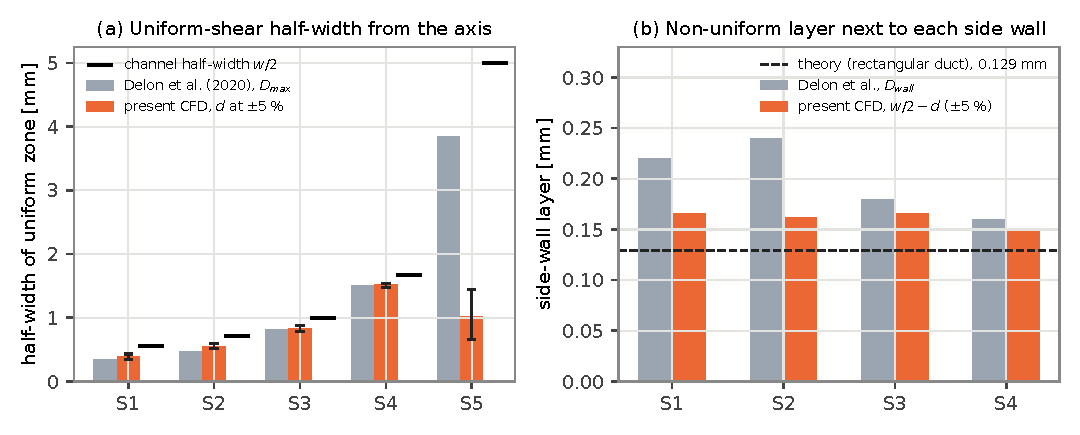
\includegraphics[width=\linewidth]{published_vs_present_uniform_zone.pdf}
\caption{Imaging zone of Delon \emph{et al.} (Table~2 of \citep{Delon2020}) compared with the present CFD at \SI{1}{\uLmin}. (a) Half-width of the uniform-shear band; error bars span the present results at $\pm2$ and $\pm\SI{10}{\percent}$ tolerance. (b) Width of the non-uniform layer at each side wall, with the rectangular-duct theory, \cref{eq:th_delta}.}
\label{fig:published_d}
\end{figure}

\paragraph{Assessment.} The published flow behaviour is reproduced \emph{qualitatively and semi-quantitatively}. The present results reproduce the linear shear decrease, the shear range at both flow rates to within a few percent, the raised minimum near the outlet, the imaging zones at S3--S4 and the independence of the flow rate. Exact agreement cannot be expected, for three reasons: the paper's own height and length are inconsistent (\cref{ch:lit}), its curves are available only as plots, and its uniformity criterion is not specified.

\section{Pressure distribution}
\label{sec:val_pressure}

\Cref{fig:contours}a shows the Fluent pressure contours. The pressure falls smoothly from inlet to outlet. Iso-bars are straight across the narrow part, as \cref{eq:th_dpdx_general} assumes, and bend only near the outlet corner, where the flow becomes two-dimensional. The colour-bar maxima scale with $Q$ to within \SI{0.3}{\percent} (1.795--\SI{1.800}{Pa} per \ulmin).

\begin{figure}[htbp]
\centering
\begin{subfigure}[t]{0.49\linewidth}\centering
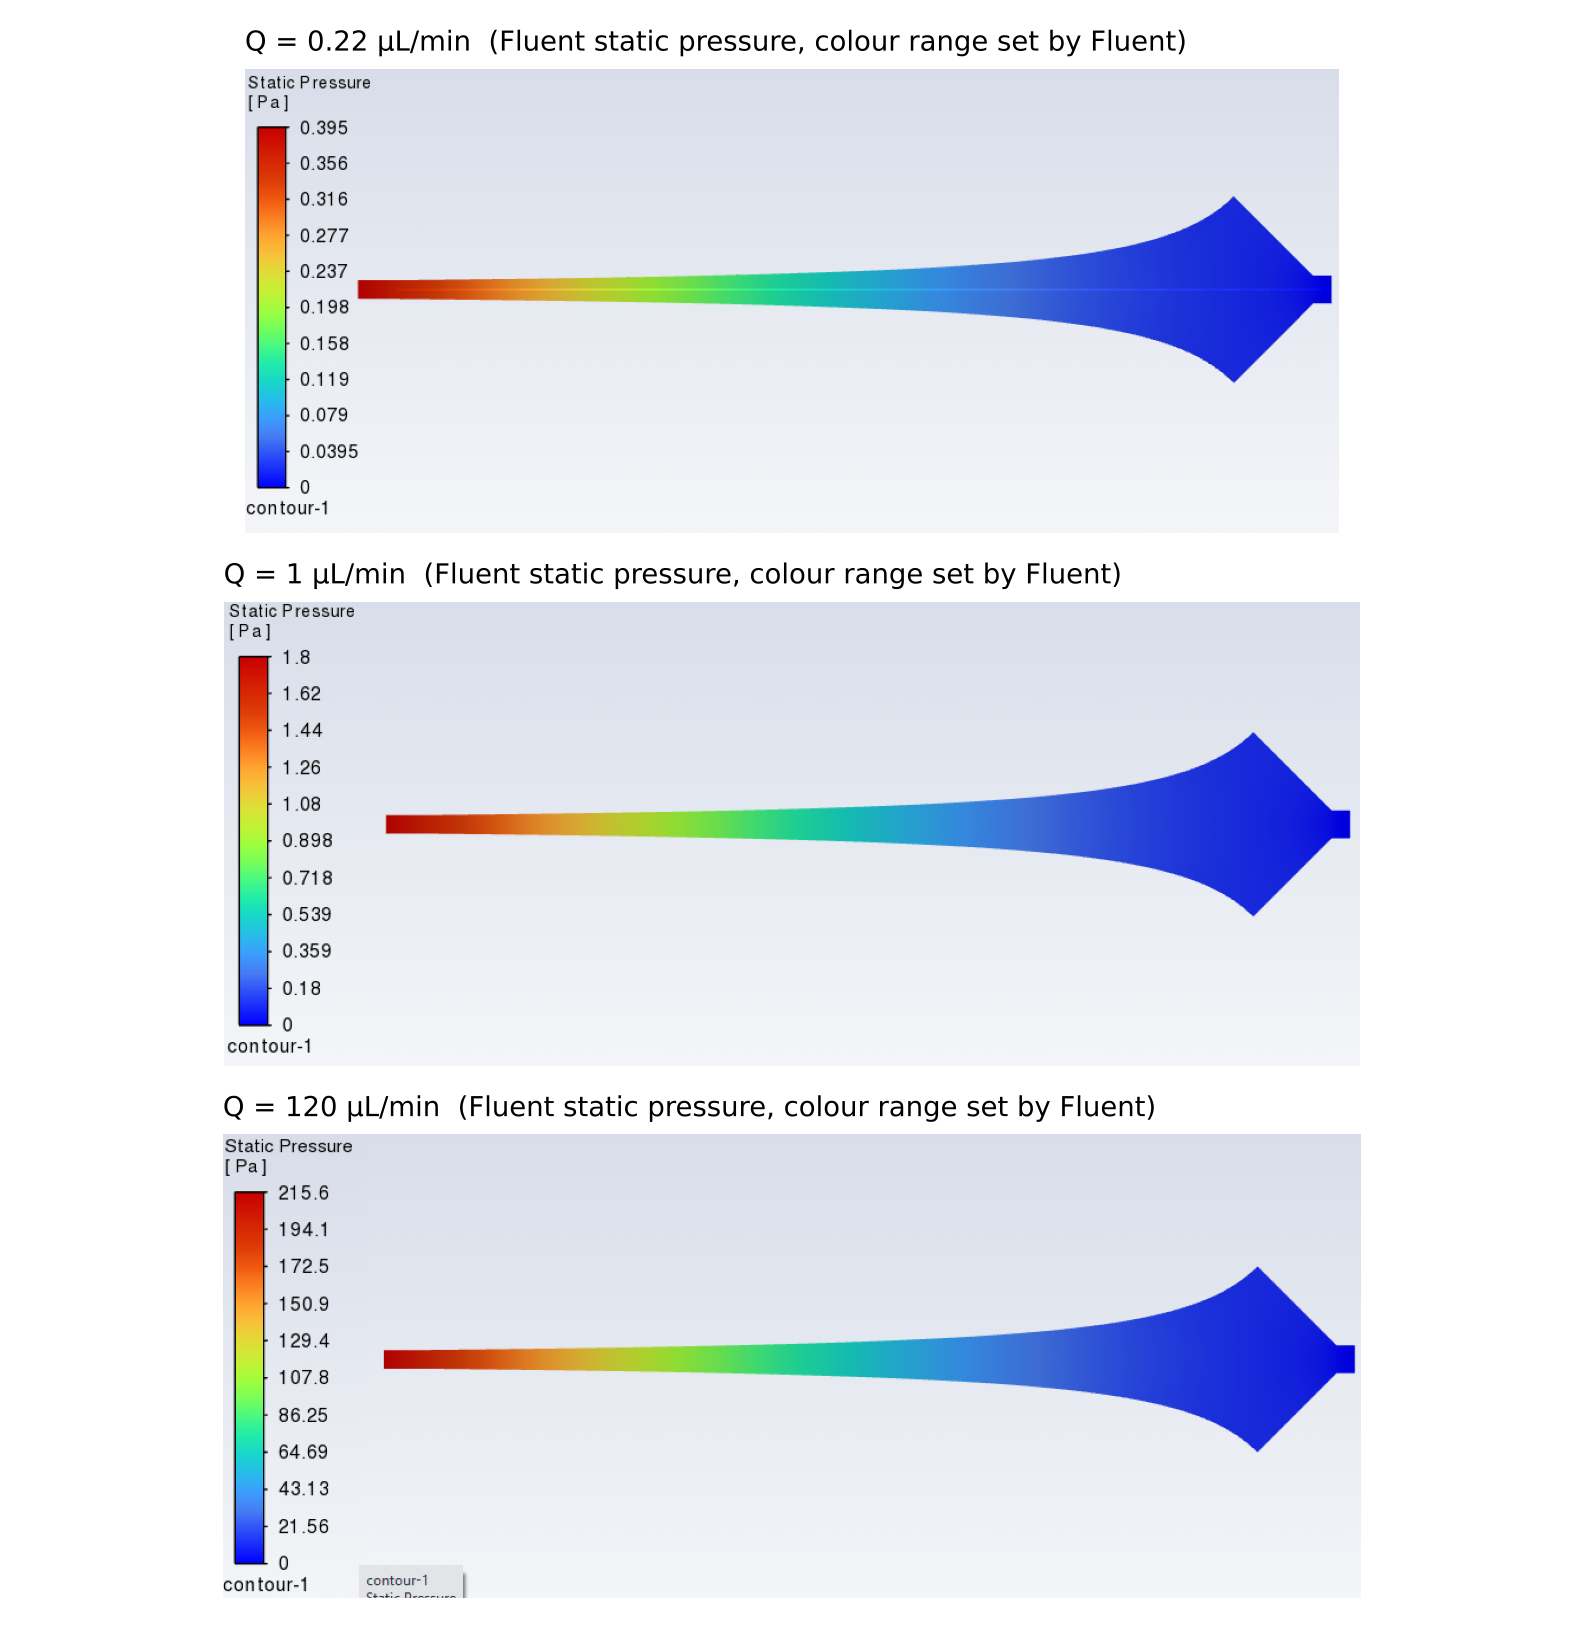
\includegraphics[width=\linewidth]{Fig01_pressure_contours_all_Q.png}
\caption{Static pressure.}
\end{subfigure}\hfill
\begin{subfigure}[t]{0.49\linewidth}\centering
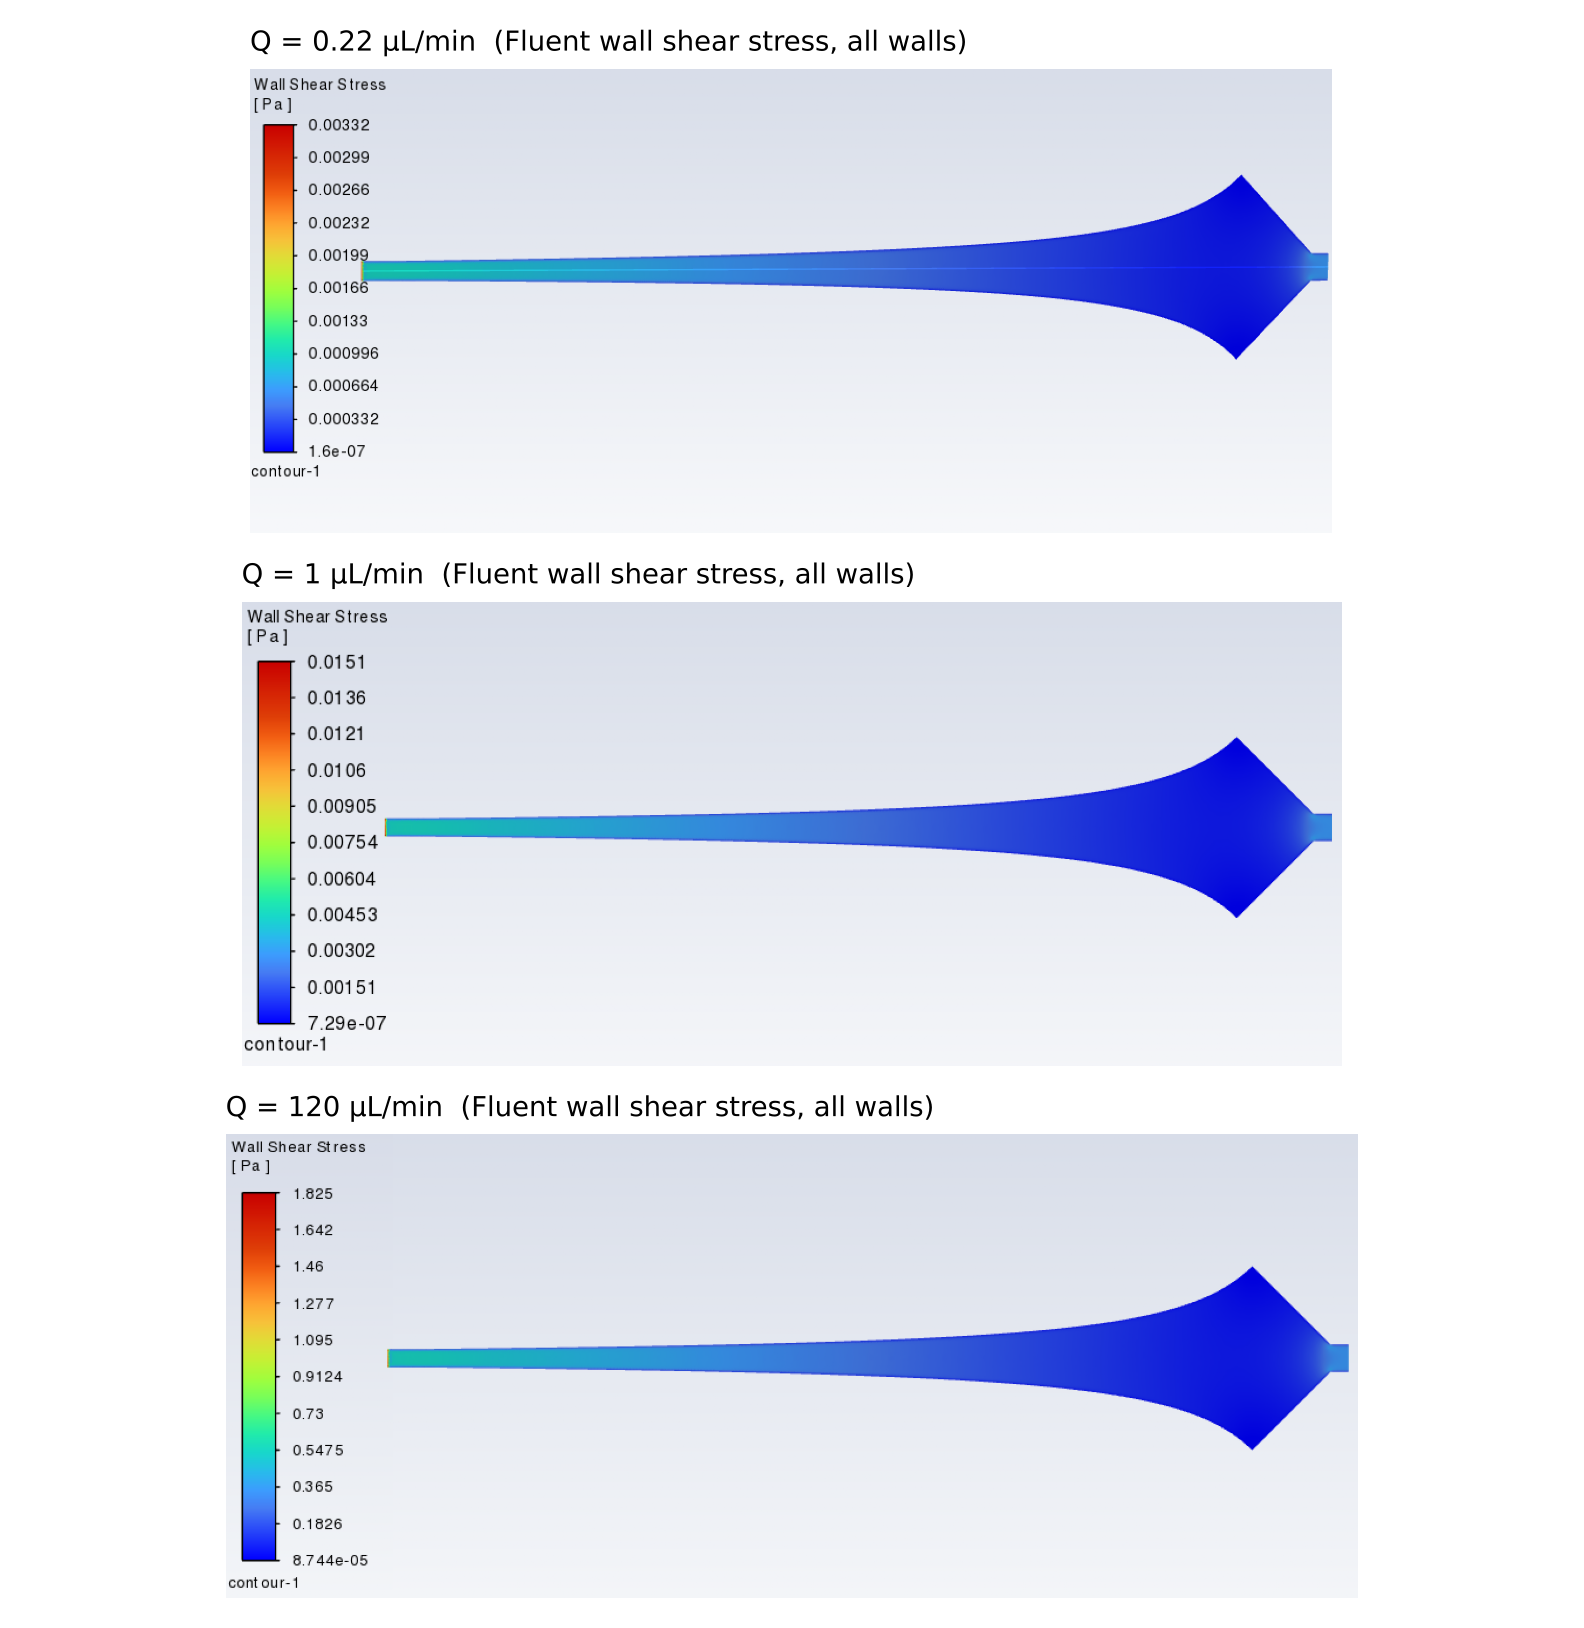
\includegraphics[width=\linewidth]{Fig09_wall_shear_contours_all_Q.png}
\caption{Wall shear stress.}
\end{subfigure}
\caption{Fluent contours at 0.22 (top), 1 (middle) and \SI{120}{\uLmin} (bottom) \tagC. These are raster screenshots with automatic colour ranges. The pressure maxima (0.395, 1.80 and \SI{215.6}{Pa}) include the \SI{2}{mm} lead-in. The wall-shear maxima (\num{3.32e-3}, \num{1.51e-2} and \SI{1.825}{Pa}) occur at the inlet face of the lead-in, where the uniform inlet velocity creates a local peak. This peak dominates the colour scale, so the shear gradient along the cell floor is quantified in the line plots that follow.}
\label{fig:contours}
\end{figure}

\Cref{fig:p_axis} compares the axial pressure at \SI{1}{\uLmin} with the theory. It decreases monotonically: none of the 729 successive differences is positive in any case. The profile flattens along the widening section, because a wider channel needs a smaller gradient for the same flow, and it steepens again where the walls converge to the outlet. T3 reproduces the whole shape, including the outlet region, but lies about \SI{5}{\percent} above the CFD everywhere. Normalised by $Q$, the three cases collapse onto one curve (\cref{fig:p_norm}). The pressure drop from $x=0$ to the outlet is $\Delta p=1.657\,Q$ (Pa, $Q$ in \ulmin) with $R^2=1.000000$ (\cref{fig:dp_Q}). The hydraulic resistance is \SI{9.94e10}{Pa.s/m^3} at all three flow rates, varying by only \SI{0.02}{\percent}.

\begin{figure}[htbp]
\centering
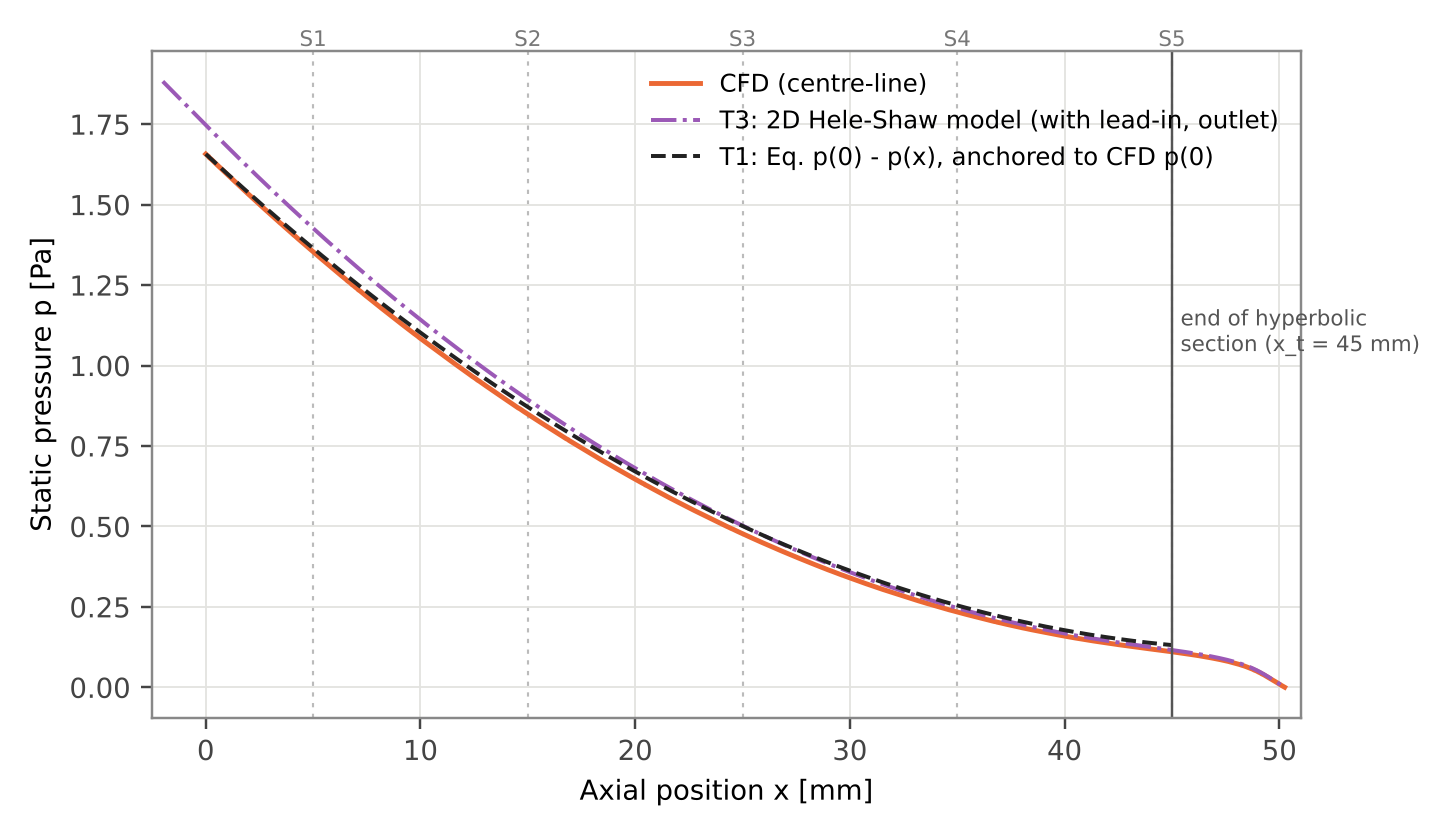
\includegraphics[width=0.85\linewidth]{Fig03_pressure_vs_x_Q1.png}
\caption{Static pressure along the axis at \SI{1}{\uLmin}: CFD \tagC\ against T3 (absolute; includes the lead-in and the outlet transition) and T1, \cref{eq:th_p}, anchored at the CFD value at $x=0$ \tagT. T1 applies only to $0\le x\le\SI{45}{mm}$.}
\label{fig:p_axis}
\end{figure}

\begin{figure}[htbp]
\centering
\begin{subfigure}[t]{0.49\linewidth}\centering
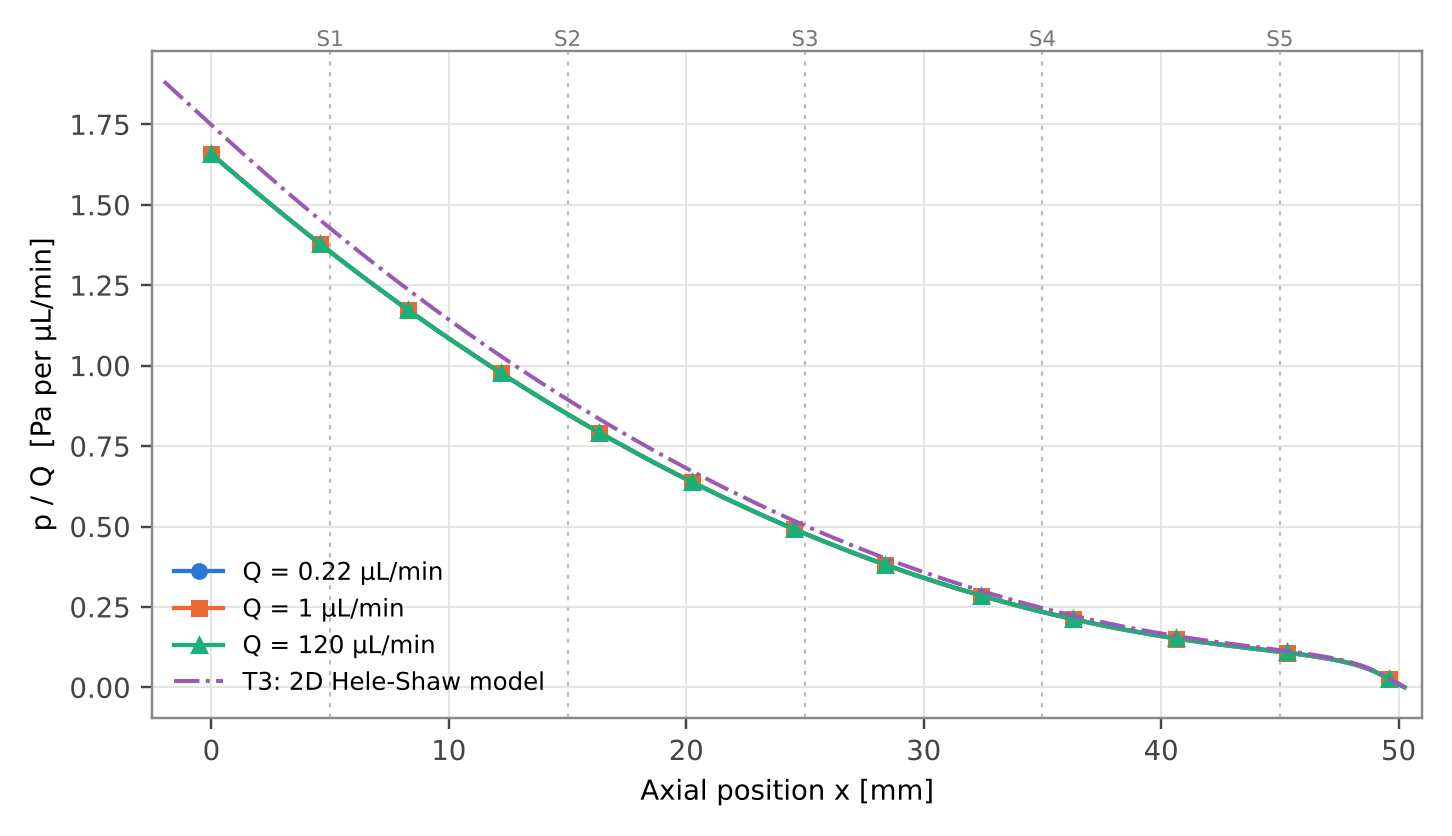
\includegraphics[width=\linewidth]{Fig05_pressure_vs_x_combined_normalised.png}
\caption{Pressure divided by $Q$.}\label{fig:p_norm}
\end{subfigure}\hfill
\begin{subfigure}[t]{0.49\linewidth}\centering
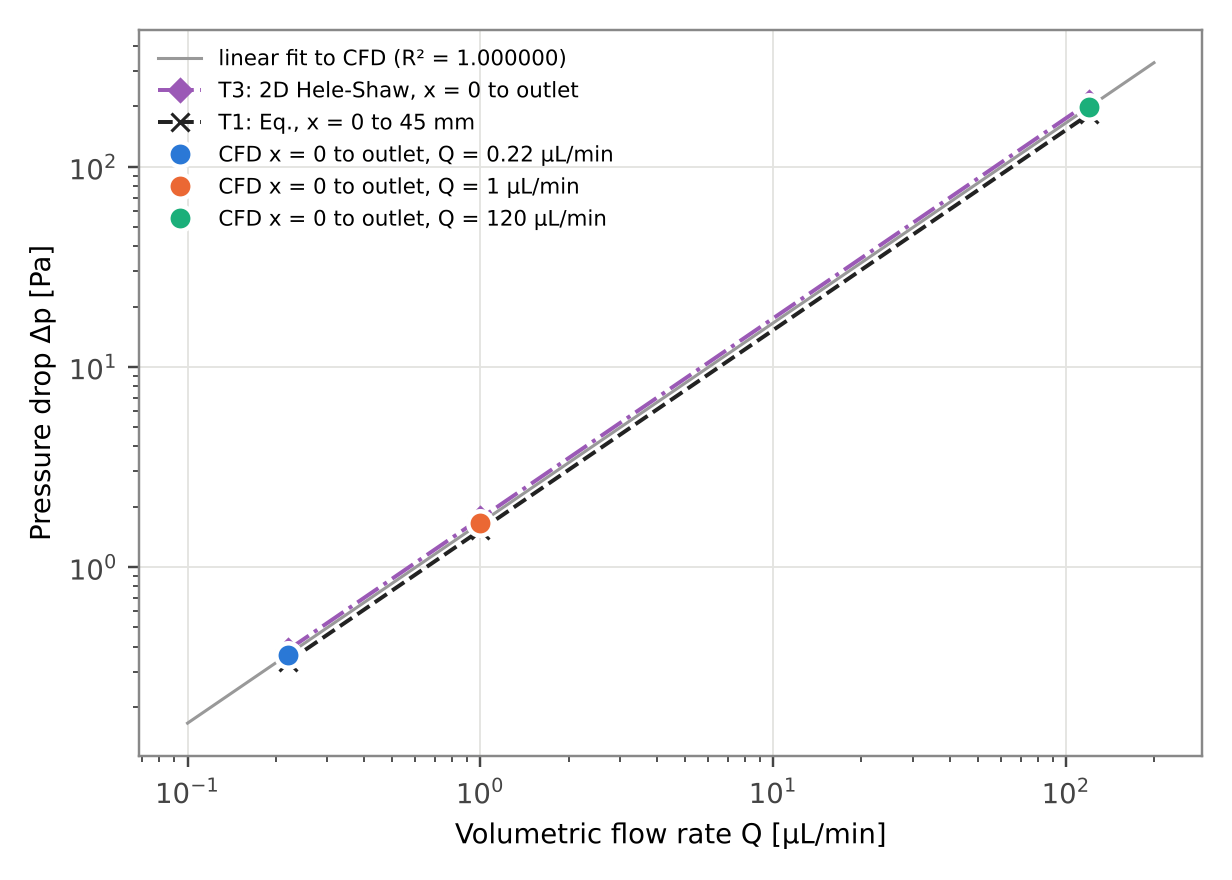
\includegraphics[width=\linewidth]{Fig06_pressure_drop_vs_Q.png}
\caption{Pressure drop against $Q$.}\label{fig:dp_Q}
\end{subfigure}
\caption{Flow-rate scaling of the pressure \tagC. (a) The three axial profiles divided by $Q$ collapse to within \SI{0.02}{\percent}; T3 lies about \SI{5}{\percent} above. (b) The pressure drop from $x=0$ to the outlet is proportional to $Q$ over a factor of 545. The T1 points cover only the hyperbolic section and are therefore lower by construction.}
\end{figure}

\paragraph{Local pressure gradient.} The gradient (\cref{fig:dpdx}, \cref{tab:dpdx}) falls from \SI{63}{Pa/m} per \ulmin\ at $x=0$ to a minimum of \SI{8.7}{Pa/m} per \ulmin\ at $x=\SI{43.9}{mm}$, a factor of 7.3, and then rises steeply in the outlet duct. T1 predicts a factor of 10 at $x=\SI{45}{mm}$. The minimum occurs before the end of the hyperbola because the flow already starts to converge towards the outlet; T3 places it at \SI{44.1}{mm}. Along the hyperbolic section the CFD gradient \emph{crosses} the T1 line: it is \SI{3.3}{\percent} above T1 at S1 and \SI{2.7}{\percent} below at S4. By contrast it is 4.6--\SI{5.4}{\percent} below T2 at every station. The variation relative to T1 is the side-wall effect, which weakens as the channel widens. The constant offset relative to T2 is discussed in \cref{sec:val_offset}.

\begin{figure}[htbp]
\centering
\begin{subfigure}[t]{0.49\linewidth}\centering
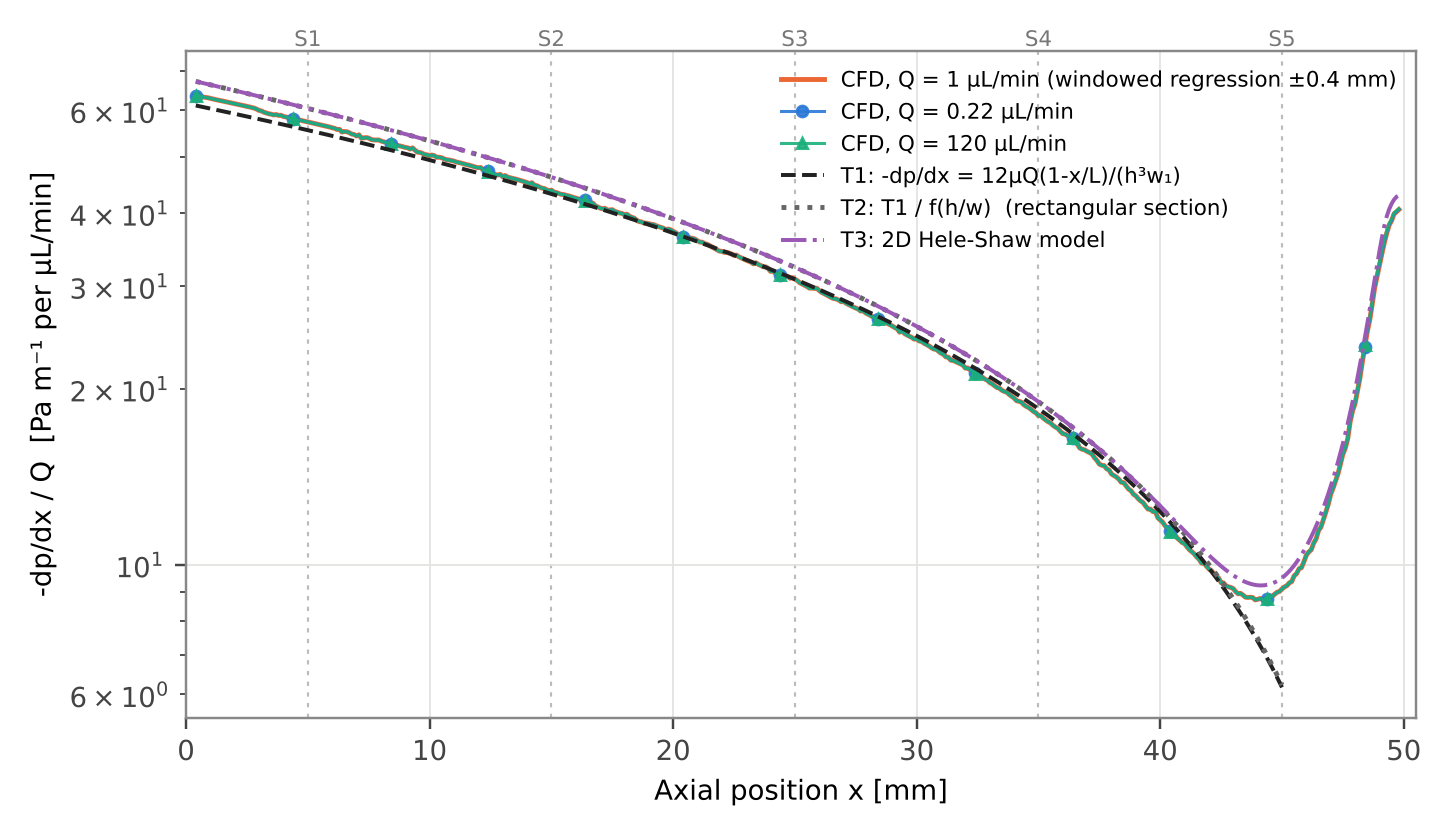
\includegraphics[width=\linewidth]{Fig07_pressure_gradient_vs_x.png}
\caption{Local gradient per unit flow rate.}\label{fig:dpdx}
\end{subfigure}\hfill
\begin{subfigure}[t]{0.49\linewidth}\centering
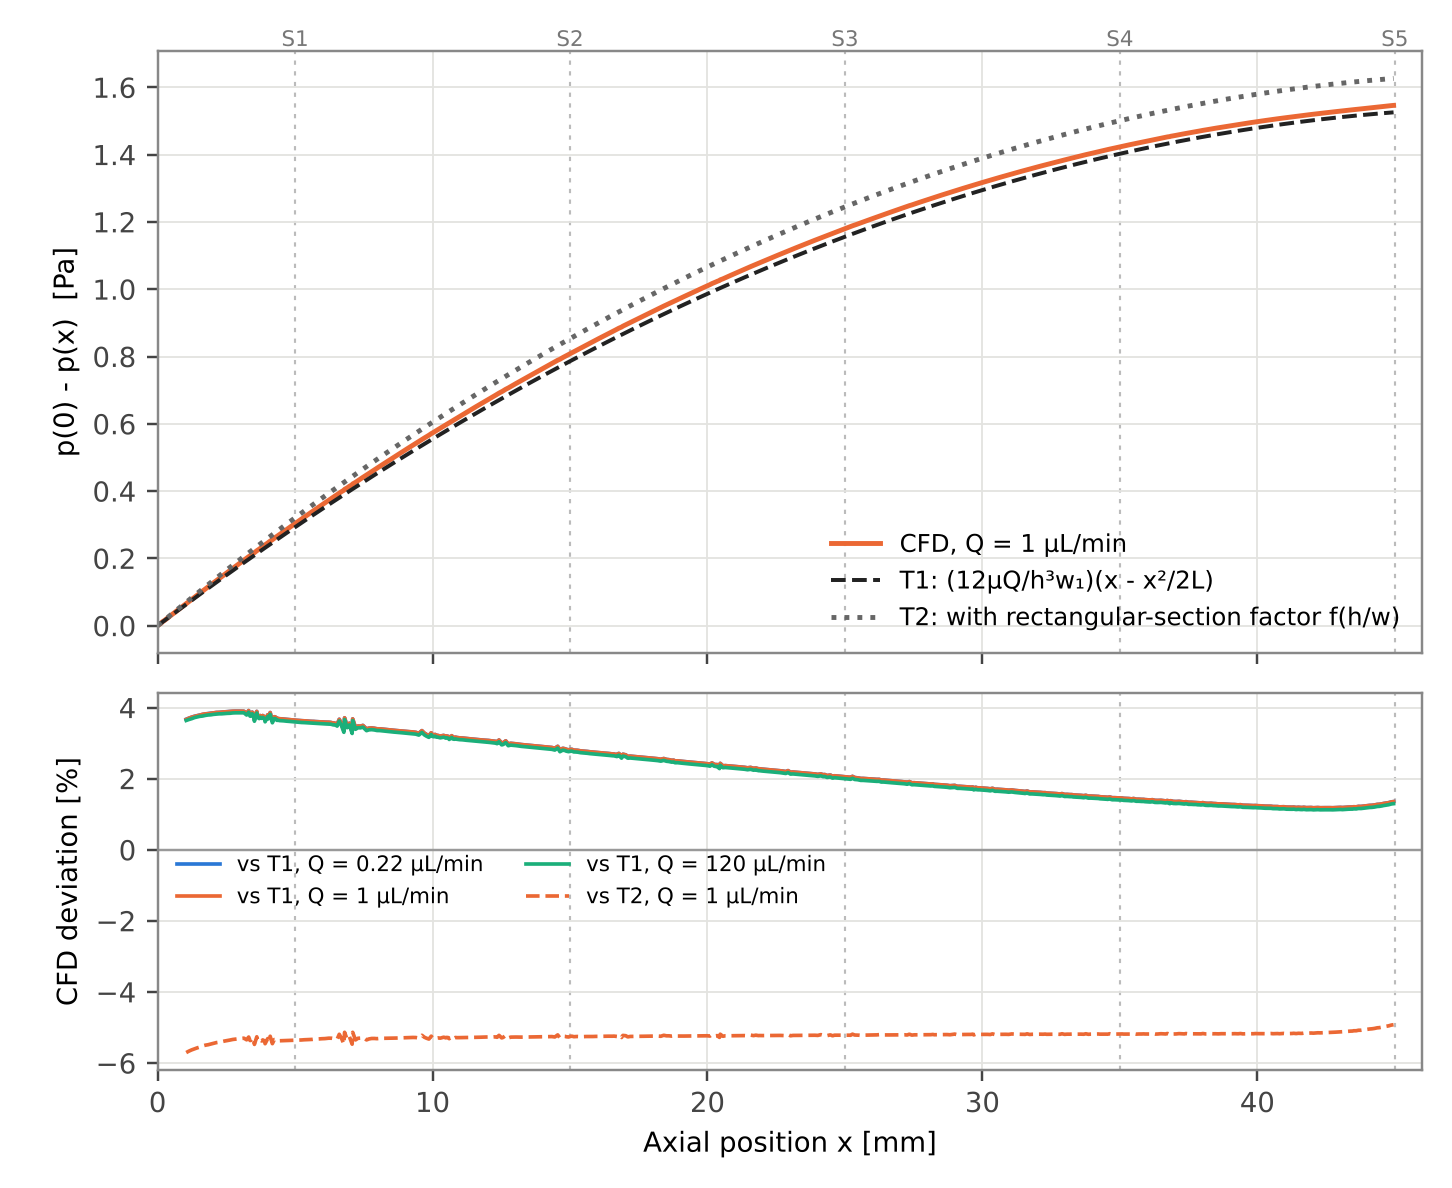
\includegraphics[width=\linewidth]{Fig08_pressure_drop_CFD_vs_theory.png}
\caption{Cumulative drop and deviation from theory.}\label{fig:dp_theory}
\end{subfigure}
\caption{Pressure gradient and cumulative pressure drop \tagC\ against theory \tagT. (a) $|\dd p/\dd x|/Q$ from a $\pm\SI{0.4}{mm}$ least-squares window; the gradient falls linearly with $x$, reaches a minimum at $x\approx\SI{44}{mm}$ and rises in the converging outlet. (b) Top: $p(0)-p(x)$ at \SI{1}{\uLmin} against \cref{eq:th_p}. Bottom: signed deviation from T1 (the three flow rates coincide) and from T2. Over 0--\SI{45}{mm} the CFD is \SI{1.4}{\percent} above T1 and \SI{4.9}{\percent} below T2.}
\end{figure}

\begin{table}[htbp]
\centering
\caption{Pressure gradient at the stations, \SI{1}{\uLmin} (other flow rates identical to within \SI{0.1}{\percent}). T1 and T2 do not apply at S5.}
\label{tab:dpdx}
\small
\begin{tabular}{@{}lcccccc@{}}
\toprule
Station & $h/w$ & $-\dd p/\dd x$ CFD & T1 & Dev.\ vs T1 & T2 & Dev.\ vs T2\\
 & & [Pa/m] & [Pa/m] & [\%] & [Pa/m] & [\%]\\
\midrule
S1 & 0.1305 & 57.32 & 55.49 & $+3.30$ & 60.46 & $-5.20$\\
S2 & 0.1015 & 43.81 & 43.16 & $+1.51$ & 46.11 & $-4.98$\\
S3 & 0.0725 & 30.83 & 30.83 & $+0.01$ & 32.30 & $-4.56$\\
S4 & 0.0435 & 18.00 & 18.50 & $-2.68$ & 19.02 & $-5.35$\\
S5 & 0.0145 & 9.09 & 6.17 & $+47.4$ & 6.22 & $+46.1$\\
\bottomrule
\end{tabular}
\end{table}

\begin{table}[htbp]
\centering
\caption{Pressure summary \tagC/\tagT. CFD values are axial gauge pressures. T1 covers only the hyperbolic section; T3 includes the outlet transition.}
\label{tab:pressure_summary}
\small
\begin{tabular}{@{}lccc@{}}
\toprule
Quantity & \SI{0.22}{\uLmin} & \SI{1}{\uLmin} & \SI{120}{\uLmin}\\
\midrule
$p(x=0)$, CFD [Pa] & 0.3647 & 1.6574 & 198.93\\
$\Delta p_{0-45}$, CFD [Pa] & 0.3404 & 1.5468 & 185.59\\
$\Delta p_{0-45}$, T1 [Pa] & 0.3358 & 1.5260 & 183.19\\
$\Delta p_{0-45}$, T2 [Pa] & 0.3580 & 1.6267 & 195.28\\
CFD vs T1 / vs T2 [\%] & $+1.37$ / $-4.91$ & $+1.37$ / $-4.91$ & $+1.31$ / $-4.97$\\
$\Delta p_{0-\mathrm{outlet}}$, CFD / T3 [Pa] & 0.3646 / 0.3845 & 1.6569 / 1.7475 & 198.88 / 209.78\\
CFD vs T3 [\%] & $-5.18$ & $-5.18$ & $-5.20$\\
\bottomrule
\end{tabular}
\end{table}

\section{Wall shear stress along the axis}
\label{sec:val_shear}

\Cref{fig:tau_axis} shows the axial wall shear at \SI{1}{\uLmin} against T1, T2 and T3. The CFD decreases almost linearly from \SI{4.62}{mPa} per \ulmin\ at $x=0$ to a minimum of \SI{0.630}{mPa} per \ulmin\ at $x=\SI{44.0}{mm}$ (T3: \SI{44.1}{mm}), then rises to \SI{3.03}{mPa} per \ulmin\ in the outlet duct. \Cref{tab:shear_stations} gives the station values for all three flow rates.

\begin{figure}[htbp]
\centering
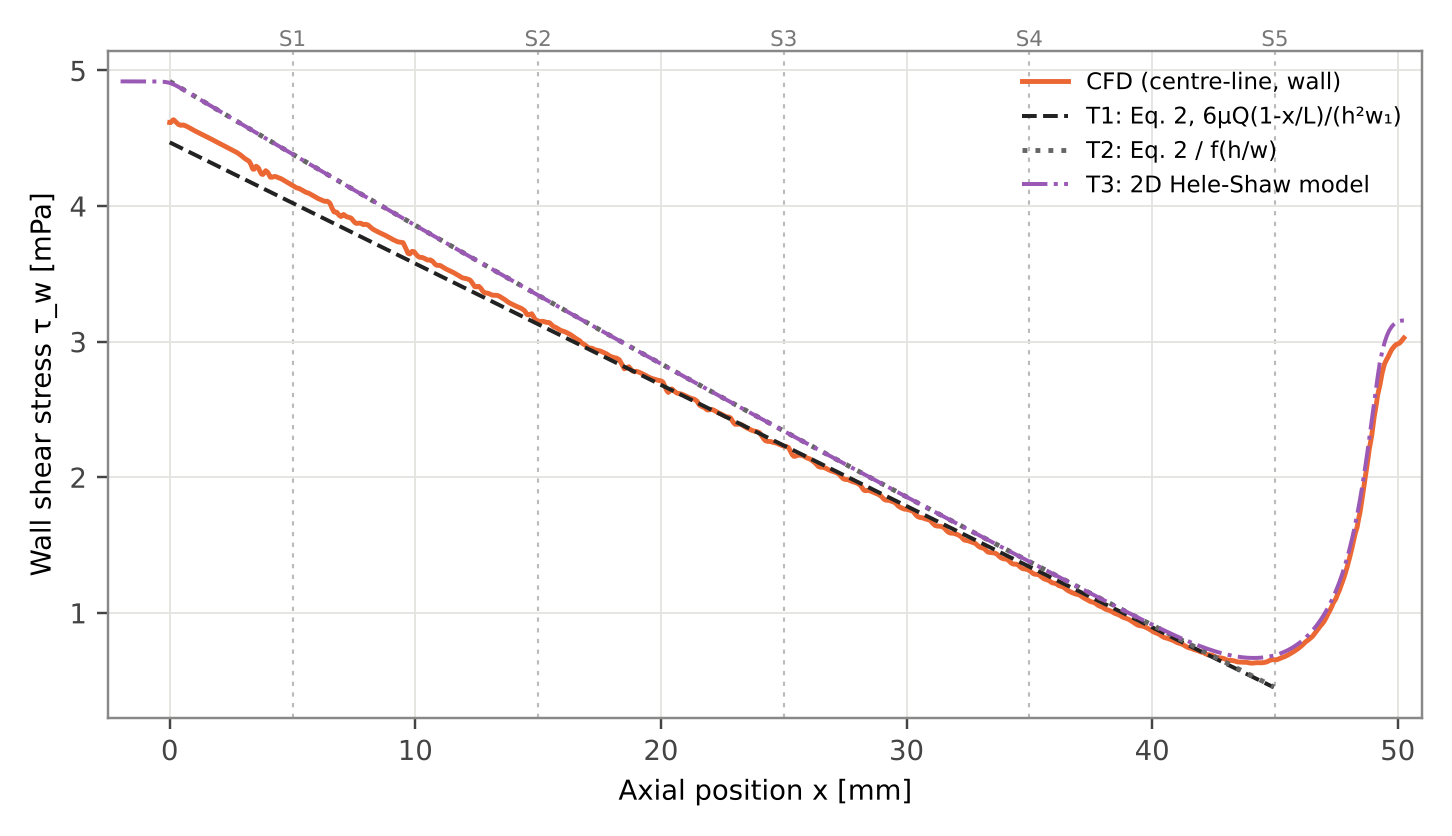
\includegraphics[width=0.88\linewidth]{Fig11_wall_shear_vs_x_Q1.png}
\caption{Wall shear on the axis at \SI{1}{\uLmin}: CFD \tagC\ against Eq.~2 (T1), the side-wall-corrected theory (T2) and the 2D model (T3) \tagT. The CFD lies above T1 near the inlet and below it near S4, and runs parallel to T2/T3 about \SI{5}{\percent} lower. Beyond $x\approx\SI{42}{mm}$ the CFD and T3 rise away from T1.}
\label{fig:tau_axis}
\end{figure}

\begin{table}[htbp]
\centering
\caption{Axial wall shear at the stations compared with Eq.~2 (T1) for all flow rates. Signed deviation $=\tau_{\mathrm{CFD}}/\tau_{T1}-1$. Deviations from T2 and T3 are given for reference.}
\label{tab:shear_stations}
\small
\begin{tabular}{@{}llccccc@{}}
\toprule
Station & $Q$ [\ulmin] & $\taw$ CFD [Pa] & $\taw$ T1 [Pa] & Dev.\ T1 [\%] & Dev.\ T2 [\%] & Dev.\ T3 [\%]\\
\midrule
S1 & 0.22 & \num{9.140e-4} & \num{8.852e-4} & $+3.25$ & $-5.24$ & $-5.24$\\
S2 & 0.22 & \num{6.935e-4} & \num{6.885e-4} & $+0.72$ & $-5.72$ & $-5.71$\\
S3 & 0.22 & \num{4.908e-4} & \num{4.918e-4} & $-0.21$ & $-4.77$ & $-4.75$\\
S4 & 0.22 & \num{2.888e-4} & \num{2.951e-4} & $-2.12$ & $-4.80$ & $-4.79$\\
S5 & 0.22 & \num{1.441e-4} & \num{9.836e-5} & $+46.47$ & n/a & $-4.87$\\
\addlinespace
S1 & 1 & \num{4.154e-3} & \num{4.023e-3} & $+3.25$ & $-5.24$ & $-5.23$\\
S2 & 1 & \num{3.152e-3} & \num{3.129e-3} & $+0.72$ & $-5.72$ & $-5.71$\\
S3 & 1 & \num{2.230e-3} & \num{2.235e-3} & $-0.21$ & $-4.77$ & $-4.75$\\
S4 & 1 & \num{1.313e-3} & \num{1.341e-3} & $-2.12$ & $-4.81$ & $-4.79$\\
S5 & 1 & \num{6.547e-4} & \num{4.470e-4} & $+46.47$ & n/a & $-4.87$\\
\addlinespace
S1 & 120 & \num{4.988e-1} & \num{4.830e-1} & $+3.29$ & $-5.21$ & $-5.20$\\
S2 & 120 & \num{3.784e-1} & \num{3.756e-1} & $+0.72$ & $-5.72$ & $-5.71$\\
S3 & 120 & \num{2.677e-1} & \num{2.683e-1} & $-0.22$ & $-4.78$ & $-4.77$\\
S4 & 120 & \num{1.575e-1} & \num{1.610e-1} & $-2.14$ & $-4.83$ & $-4.81$\\
S5 & 120 & \num{7.859e-2} & \num{5.366e-2} & $+46.46$ & n/a & $-4.87$\\
\bottomrule
\end{tabular}
\end{table}

\paragraph{Error metrics.} Over the central region $2\le x\le\SI{40}{mm}$ (about 570 points), the CFD deviates from the three theories as follows (identical at all $Q$ to within \SI{0.02}{\percent}):

\begin{center}
\small
\begin{tabular}{@{}lccc@{}}
\toprule
Metric (2--\SI{40}{mm}, \SI{1}{\uLmin}) & vs T1 & vs T2 & vs T3\\
\midrule
RMSE [mPa] & 0.064 & 0.156 & 0.156\\
Normalised RMSE (RMSE / mean theory) [\%] & 2.45 & 5.62 & 5.61\\
Mean absolute percentage error [\%] & 1.79 & 5.16 & 5.16\\
Maximum absolute percentage error [\%] & 4.04 & 6.47 & 6.46\\
\bottomrule
\end{tabular}
\end{center}

\noindent On these metrics alone, Eq.~2 (T1) would appear to be the best theory. The next two figures show that this is misleading.

\begin{figure}[htbp]
\centering
\begin{subfigure}[t]{0.49\linewidth}\centering
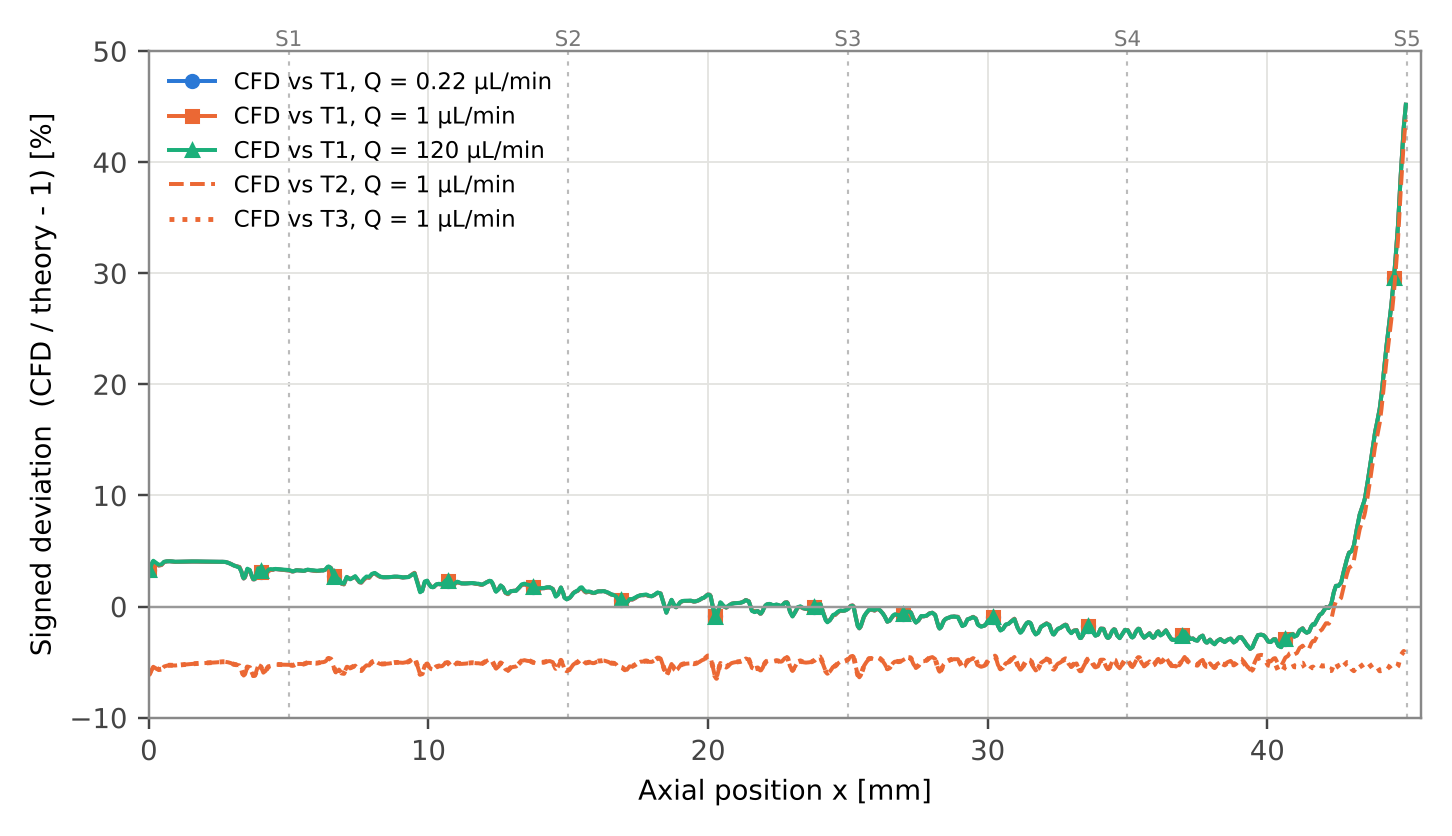
\includegraphics[width=\linewidth]{Fig15_wall_shear_percentage_deviation.png}
\caption{Signed deviation along $x$.}\label{fig:tau_dev}
\end{subfigure}\hfill
\begin{subfigure}[t]{0.49\linewidth}\centering
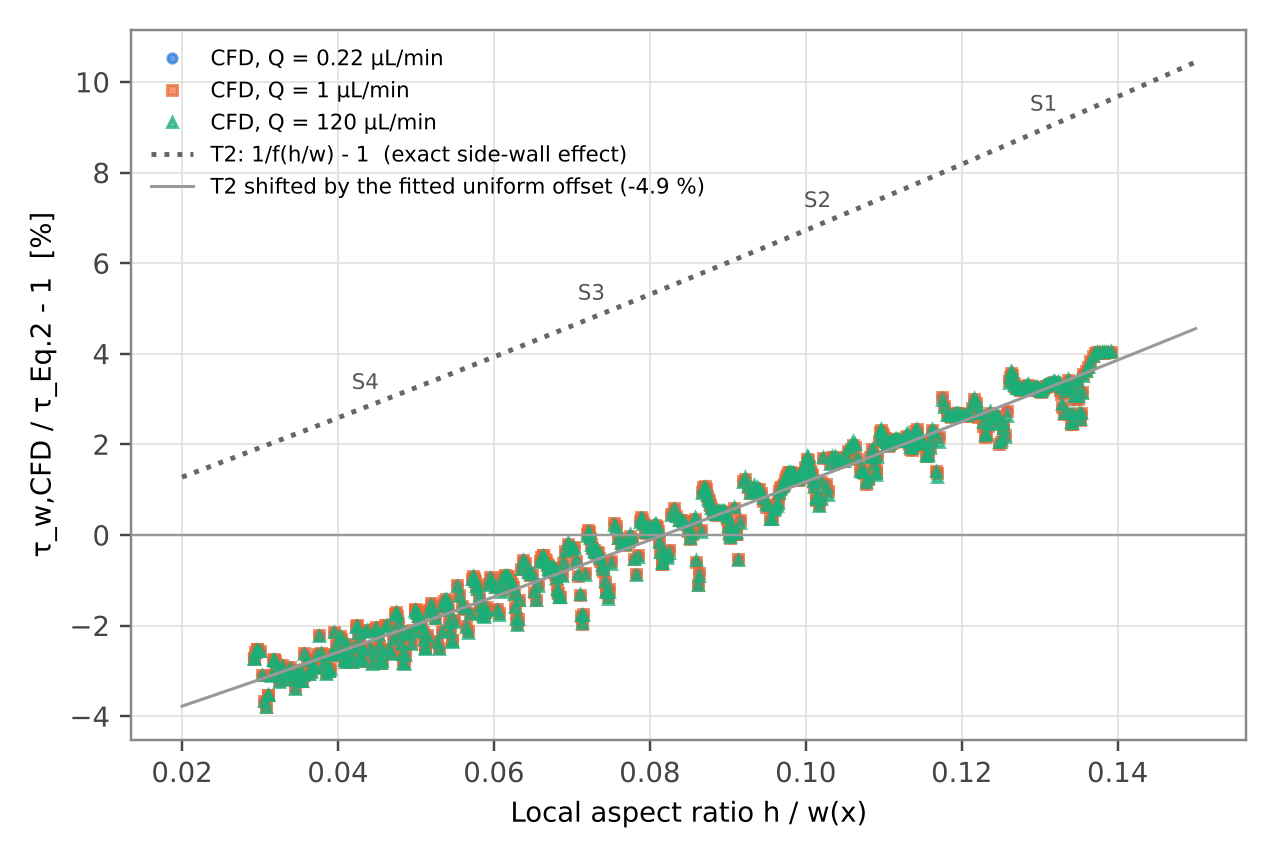
\includegraphics[width=\linewidth]{Fig16_shear_deviation_vs_aspect_ratio.png}
\caption{Deviation from Eq.~2 against $h/w$.}\label{fig:tau_hw}
\end{subfigure}
\caption{Structure of the deviation of the CFD shear from theory \tagC. (a) Against Eq.~2 the deviation runs from about \SI{+4}{\percent} at the inlet through zero at $x\approx\SI{23}{mm}$ to $-2$ to \SI{-3}{\percent} at S4--\SI{40}{mm}, then rises steeply to \SI{+46}{\percent} at S5. Against T2 it is a near-constant \SI{-5.2(4)}{\percent}; against T3 it stays at \SI{-5}{\percent} including S5. (b) Points: CFD between $x=2$ and \SI{40}{mm}. They follow a line parallel to the exact side-wall correction $1/f-1$ (slope difference only $-0.026$ per unit $h/w$), shifted by \SI{-4.9}{\percent}.}
\end{figure}

\paragraph{Why the deviation from Eq.~2 is systematic.} \Cref{fig:tau_hw} plots the deviation from Eq.~2 against the local aspect ratio. If the only error in Eq.~2 were the neglect of side walls, the points would lie on the T2 curve $1/f(h/w)-1\approx0.63\,h/w$. They lie on a line with exactly that slope (residual slope $-0.026$ per unit $h/w$, scatter \SI{\pm0.36}{\percent}), shifted down by \SI{4.9}{\percent}. The 3D CFD therefore captures the side-wall drag that Eq.~2 omits, with the correct coefficient. On top of that it carries a uniform offset. Near the inlet the two effects partly cancel (\SI{+9}{\percent} side-wall drag, \SI{-5}{\percent} offset, net \SI{+3.3}{\percent}), and near S3 they cancel exactly. The small RMSE against Eq.~2 is therefore a coincidence of two errors, not a validation of Eq.~2.

\paragraph{Linearity.} A straight line fitted to the CFD over 5--\SI{40}{mm} has $R^2=0.9996$, but it reaches zero at $x=\SI{48.8}{mm}$ rather than at $L=\SI{50}{mm}$ and departs from the data by up to \SI{5}{\percent}. The same fit applied to T2 also gives \SI{48.8}{mm}, so the curvature is physical. The side walls raise the shear most where the channel is narrowest, which steepens the decrease. The shear is linear in $x$ to within about $\pm\SI{4}{\percent}$ over the central region.

\section{Transverse distribution of the wall shear}
\label{sec:val_transverse}

\Cref{fig:transverse} shows the floor shear across the width at the five stations, and its normalised form. At S1--S4 the profile is a flat plateau (variation 0.1--\SI{0.7}{\percent} over the central half) that drops near each side wall. In absolute units the drop-off zone has the same thickness at every station. Plotted against the distance from the side wall (\cref{fig:sidewall}), the S1--S4 profiles collapse onto one curve, as \cref{eq:th_delta} predicts: the layer scales with $h$, not with $w$. At S5 there is no plateau. The shear falls continuously from the axis to near zero in the corners, because S5 is the corner of the planform. T3 reproduces this dome shape (\cref{fig:T3}).

\begin{figure}[htbp]
\centering
\begin{subfigure}[t]{0.49\linewidth}\centering
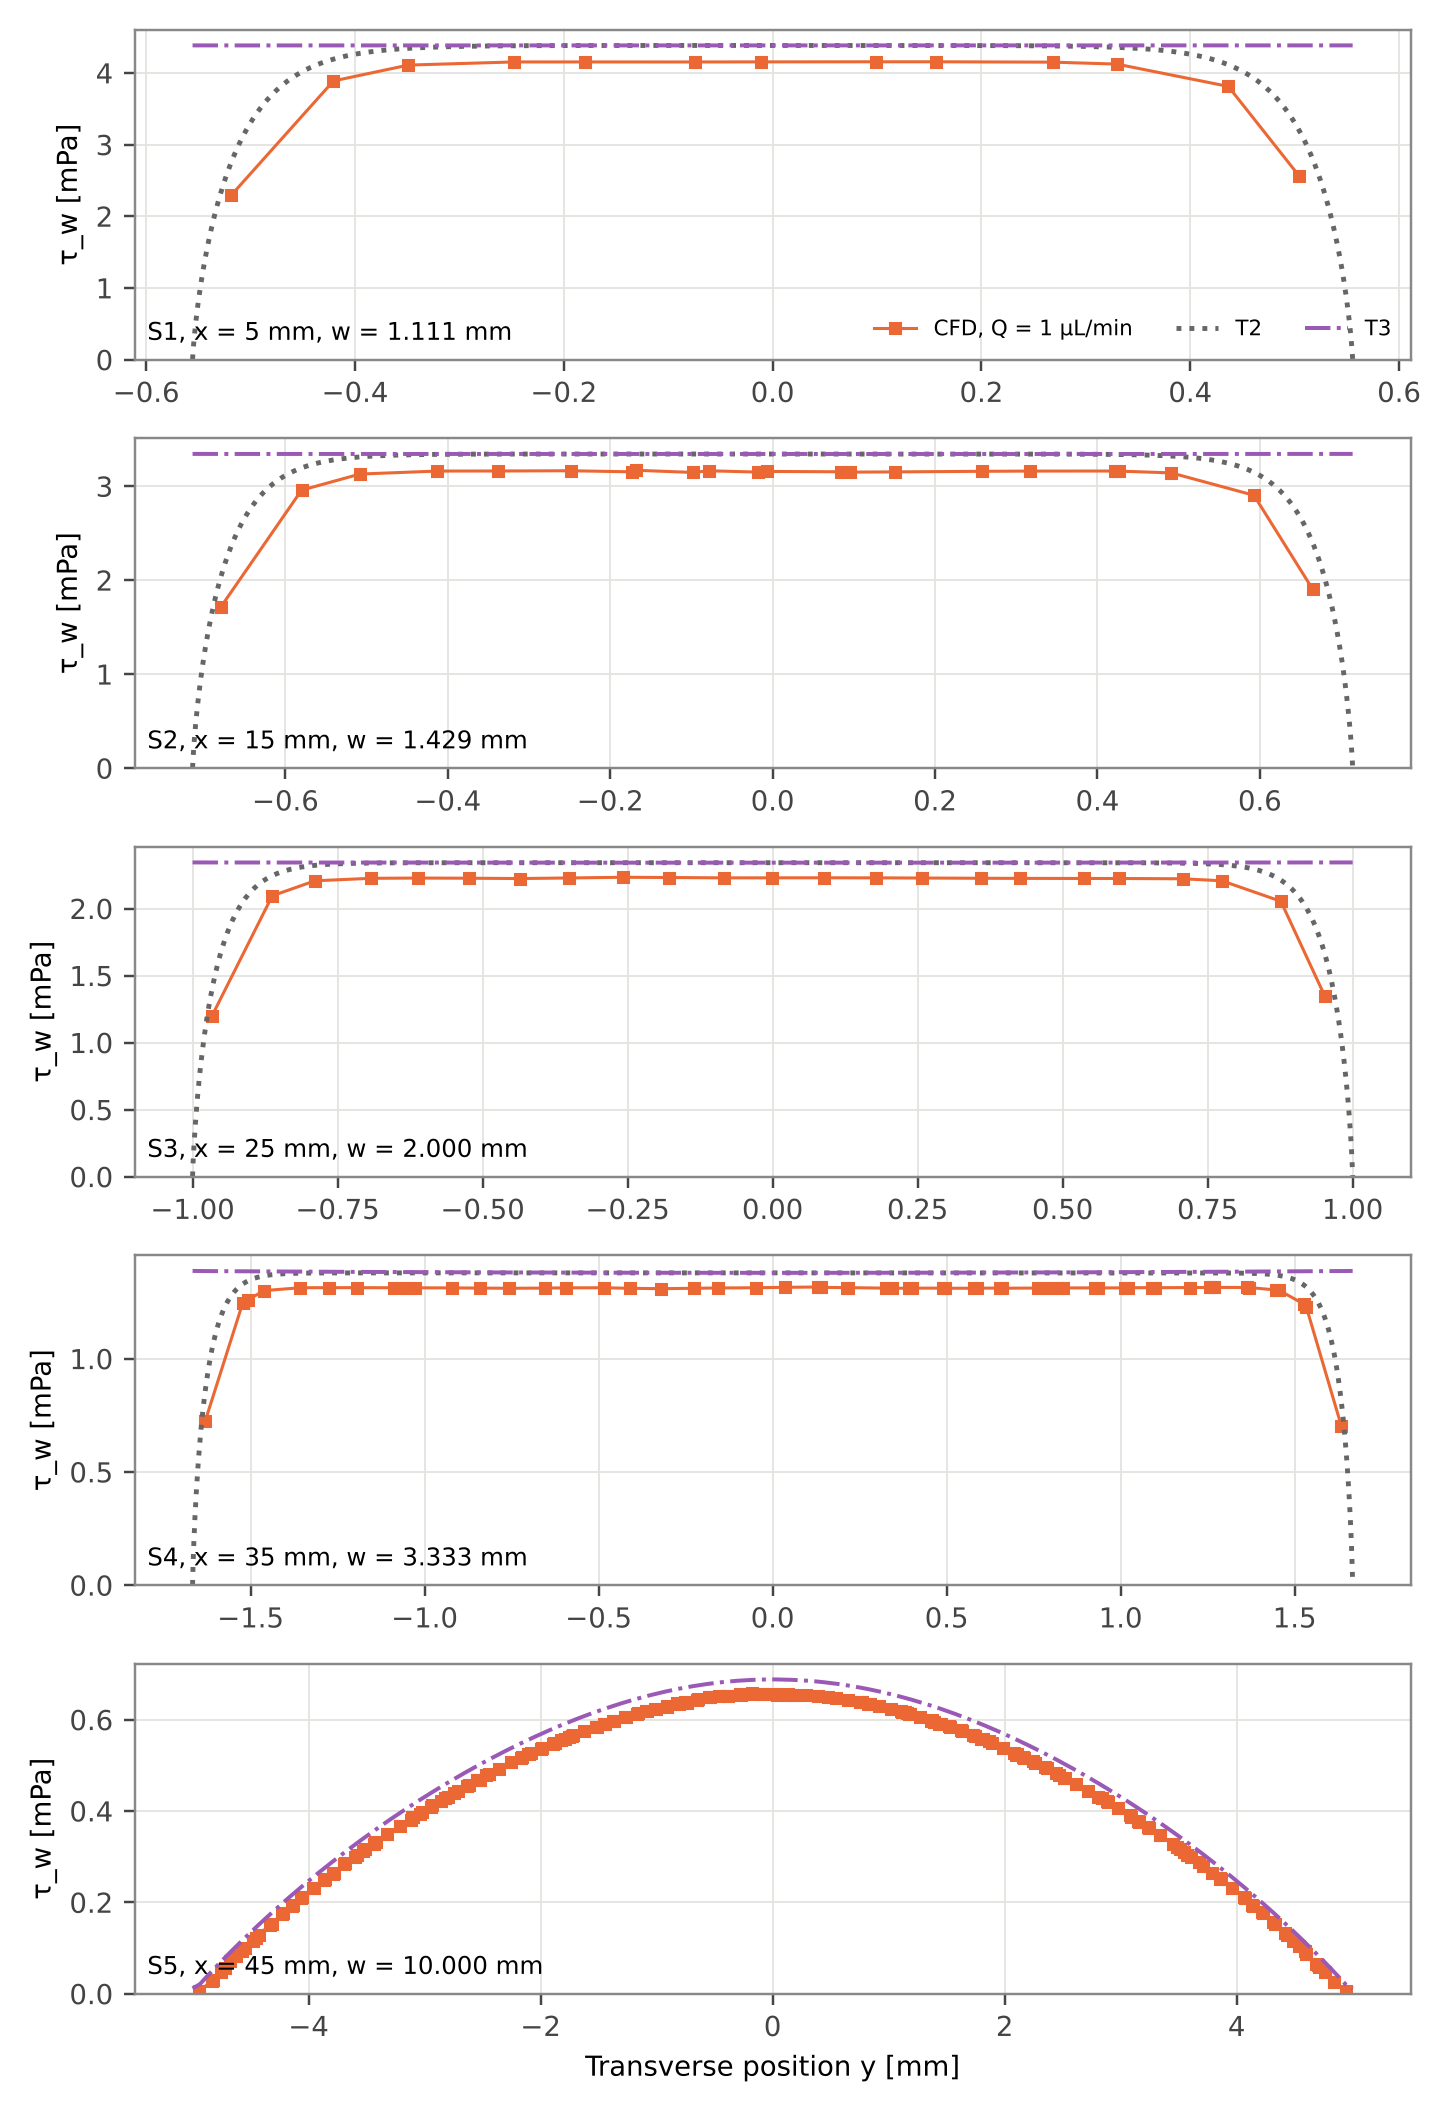
\includegraphics[width=\linewidth]{Fig22_transverse_shear_all_sections.png}
\caption{Profiles at S1--S5.}
\end{subfigure}\hfill
\begin{subfigure}[t]{0.49\linewidth}\centering
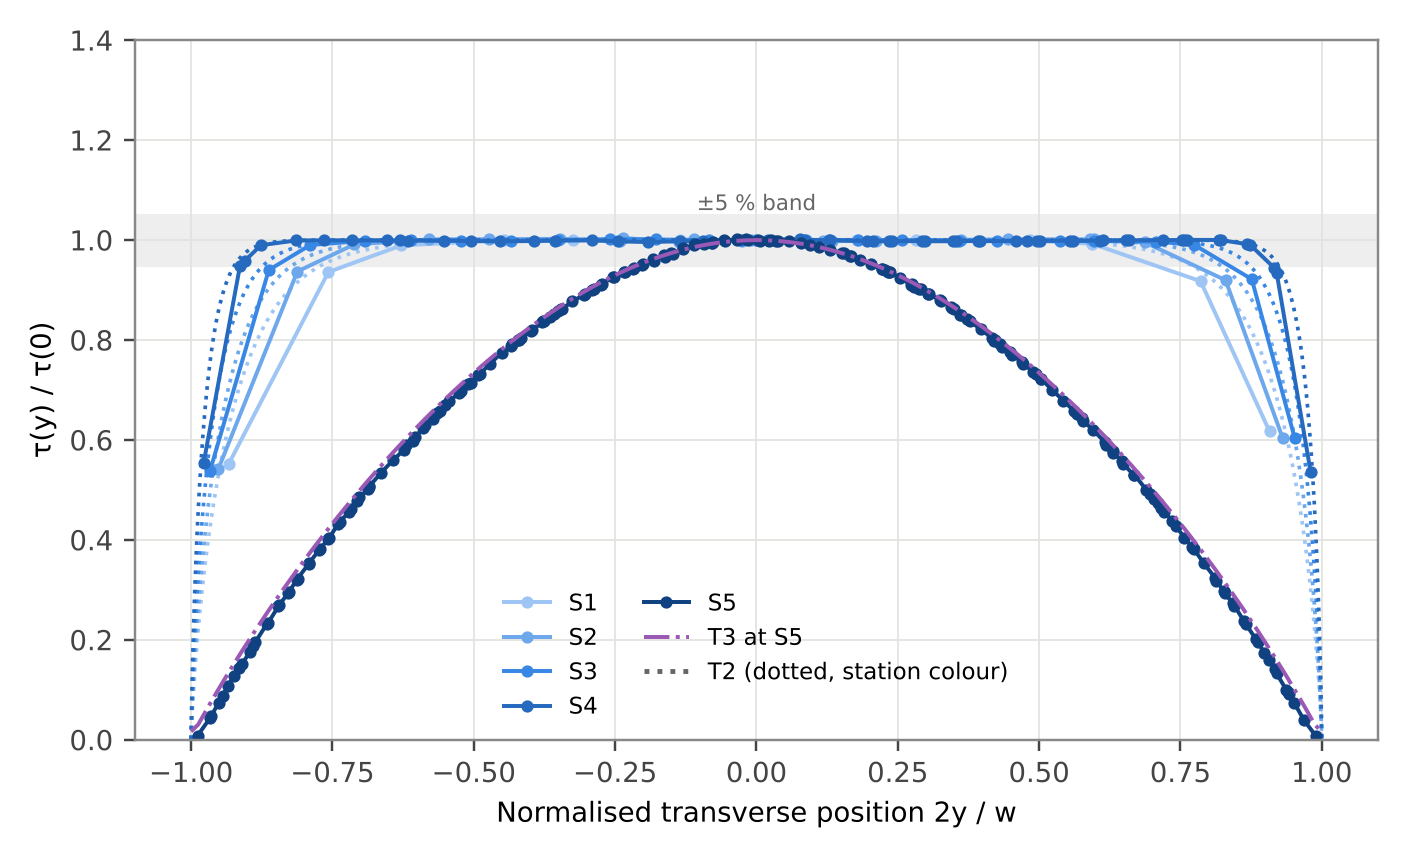
\includegraphics[width=\linewidth]{Fig24_transverse_shear_normalised.png}
\caption{Normalised by axis value and half-width.}
\end{subfigure}
\caption{Floor shear across the width at \SI{1}{\uLmin} \tagC. Each point is the mean of the coincident floor and lid wall nodes. (a) At S1--S4 a flat plateau is bounded by side-wall layers of about \SI{0.15}{mm}; at S5 the profile is a dome. (b) In the normalised coordinate $2y/w$ the plateau widens downstream, because the layer has a fixed thickness while the channel widens.}
\label{fig:transverse}
\end{figure}

\begin{figure}[htbp]
\centering
\begin{subfigure}[t]{0.49\linewidth}\centering
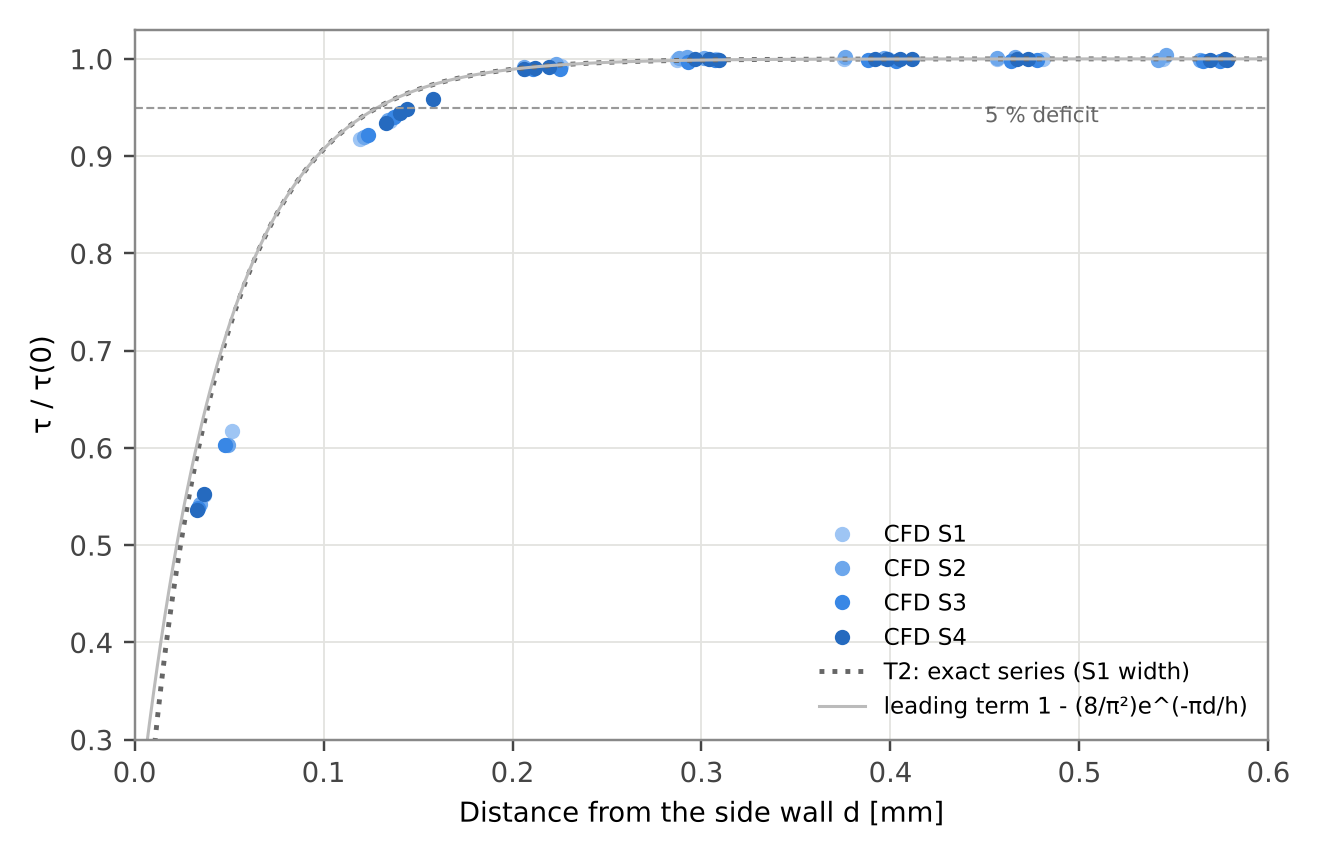
\includegraphics[width=\linewidth]{Fig25_sidewall_layer_collapse.png}
\caption{Side-wall layer collapse.}\label{fig:sidewall}
\end{subfigure}\hfill
\begin{subfigure}[t]{0.49\linewidth}\centering
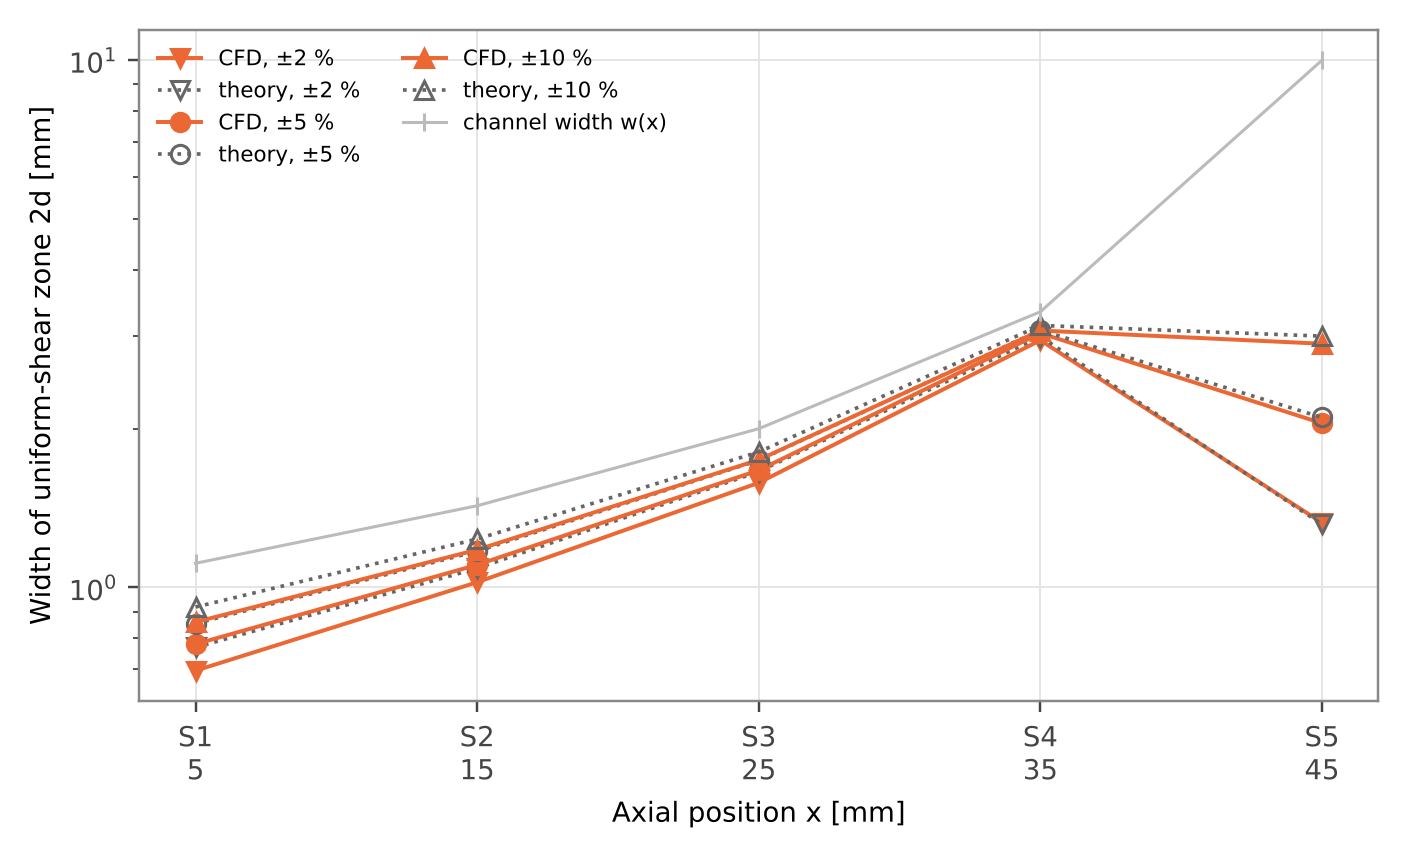
\includegraphics[width=\linewidth]{Fig26_uniform_zone_width_vs_x.png}
\caption{Uniform-zone width $2d$ and tolerance.}\label{fig:uniform}
\end{subfigure}
\caption{(a) Floor shear against the distance from the side wall at S1--S4 \tagC. The profiles collapse; the theoretical \SI{5}{\percent} point is \SI{0.129}{mm} from the wall, and the CFD wall nodes are \SIrange{0.08}{0.10}{mm} apart. (b) Width $2d$ of the central band with $|\tau(y)/\tau(0)-1|\le\varepsilon$ for $\varepsilon=2$, 5 and \SI{10}{\percent} (other flow rates differ by less than \SI{0.002}{mm}). Theory: T2 at S1--S4, T3 at S5.}
\end{figure}

\Cref{tab:uniform} quantifies the uniform zone. At S1--S4 the CFD half-width is 0.009--\SI{0.031}{mm} smaller than the theory evaluated at the same node positions. The CFD side-wall layer is \SIrange{0.149}{0.166}{mm}, against \SI{0.129}{mm} from theory. Both differences are below the \SIrange{0.08}{0.10}{mm} spacing of the exported wall nodes (\cref{tab:transverse_nodes}), so the exports confirm the theoretical layer to within their resolution but cannot resolve it more finely. The uniform fraction grows from \SI{70}{\percent} of the width at S1 to \SI{91}{\percent} at S4, and collapses to \SI{20}{\percent} at S5, in agreement with T3 (\SI{2.10}{mm} against \SI{2.05}{mm} for $2d$). The flow rate has no effect: $d$ differs by at most \SI{0.002}{mm} between 0.22 and \SI{120}{\uLmin}. The tolerance matters little at S4 (\SIrange{-3}{+1}{\percent} change in width between $\pm2$ and $\pm\SI{10}{\percent}$) but a great deal at S5 (\SIrange{-35}{+42}{\percent}), where there is no plateau.

\begin{table}[htbp]
\centering
\caption{Uniform-shear half-width $d$ at $\pm\SI{5}{\percent}$ \tagC, with theory \tagT\ (T2 at S1--S4, T3 at S5) and the sensitivity of $2d$ to the tolerance (\SI{1}{\uLmin}). Side layer $=w/2-d$.}
\label{tab:uniform}
\small
\resizebox{\linewidth}{!}{%
\begin{tabular}{@{}lcccccccc@{}}
\toprule
Station & $w/2$ & $d$ (0.22/1/120) & $2d/w$ & $d$ theory & side layer & side layer & $2d$ at $\pm2/5/10\,\%$ & $2d/w$ at\\
 & [mm] & [mm] & [\%] & [mm] & CFD [mm] & theory [mm] & [mm] & $\pm2/5/10\,\%$\\
\midrule
S1 & 0.556 & 0.390/0.390/0.389 & 70.3 & 0.427 & 0.165 & 0.129 & 0.695/0.781/0.860 & 63/70/77\\
S2 & 0.714 & 0.552/0.552/0.552 & 77.3 & 0.586 & 0.162 & 0.129 & 1.023/1.104/1.179 & 72/77/83\\
S3 & 1.000 & 0.834/0.834/0.834 & 83.4 & 0.871 & 0.166 & 0.129 & 1.579/1.668/1.746 & 79/83/87\\
S4 & 1.667 & 1.518/1.518/1.517 & 91.1 & 1.538 & 0.149 & 0.129 & 2.943/3.035/3.071 & 88/91/92\\
S5 & 5.000 & 1.024/1.024/1.025 & 20.5 & 1.050 & 3.976 & 3.950 & 1.326/2.048/2.899 & 13/20/29\\
\bottomrule
\end{tabular}}
\end{table}

\begin{table}[htbp]
\centering
\caption{Cross-section exports at \SI{1}{\uLmin}: consistency with the axial export and resolution near the side walls \tagC.}
\label{tab:transverse_nodes}
\small
\begin{tabular}{@{}lcccccc@{}}
\toprule
Station & Points & Wall nodes & $\tau(0)$ section & $\tau$ axial export & Floor--lid spread & Node spacing at\\
 & & (side/corner) & [mPa] & [mPa] & mean/max [\%] & side wall [mm]\\
\midrule
S1 & 171 & 34 (8) & 4.1542 & 4.1537 & 0.64 / 4.3 & 0.083\\
S2 & 207 & 41 (7) & 3.1571 & 3.1516 & 0.82 / 4.9 & 0.086\\
S3 & 267 & 54 (8) & 2.2291 & 2.2303 & 0.12 / 0.6 & 0.090\\
S4 & 457 & 91 (8) & 1.3143 & 1.3125 & 0.51 / 6.6 & 0.104\\
S5 & 1349 & 265 (8) & 0.6556 & 0.6547 & 0.63 / 6.7 & 0.106\\
\bottomrule
\end{tabular}
\end{table}

\section{Velocity field}
\label{sec:val_velocity}

The velocity exports contain $|\vect u|$ at all node heights plotted against $y$. Each section therefore appears as a scatter from zero up to about the mid-plane velocity. The upper envelope approximates the mid-plane profile and slightly underestimates it. At S1--S4 the walls diverge at half-angles of only \ang{0.7}--\ang{6.3}, so $|\vect u|$ exceeds $u_x$ by at most \SI{0.6}{\percent} and can be read as the axial velocity. \Cref{fig:velocity} shows a flat core with a side-wall layer of the same thickness as for the shear, as \cref{eq:th_rect_u} predicts. The peak velocity falls from \SI{0.166}{mm/s} per \ulmin\ at S1 to \SI{0.026}{mm/s} per \ulmin\ at S5, in proportion to $1/[wf(h/w)]$. The highest sampled velocity is \SIrange{1.2}{3.4}{\percent} below the theoretical mid-plane value (\cref{tab:velocity}). The pathlines (\cref{fig:pathlines}) follow the diverging walls without separation and converge smoothly into the outlet, at 1 and at \SI{120}{\uLmin}.

\begin{figure}[htbp]
\centering
\begin{subfigure}[t]{0.49\linewidth}\centering
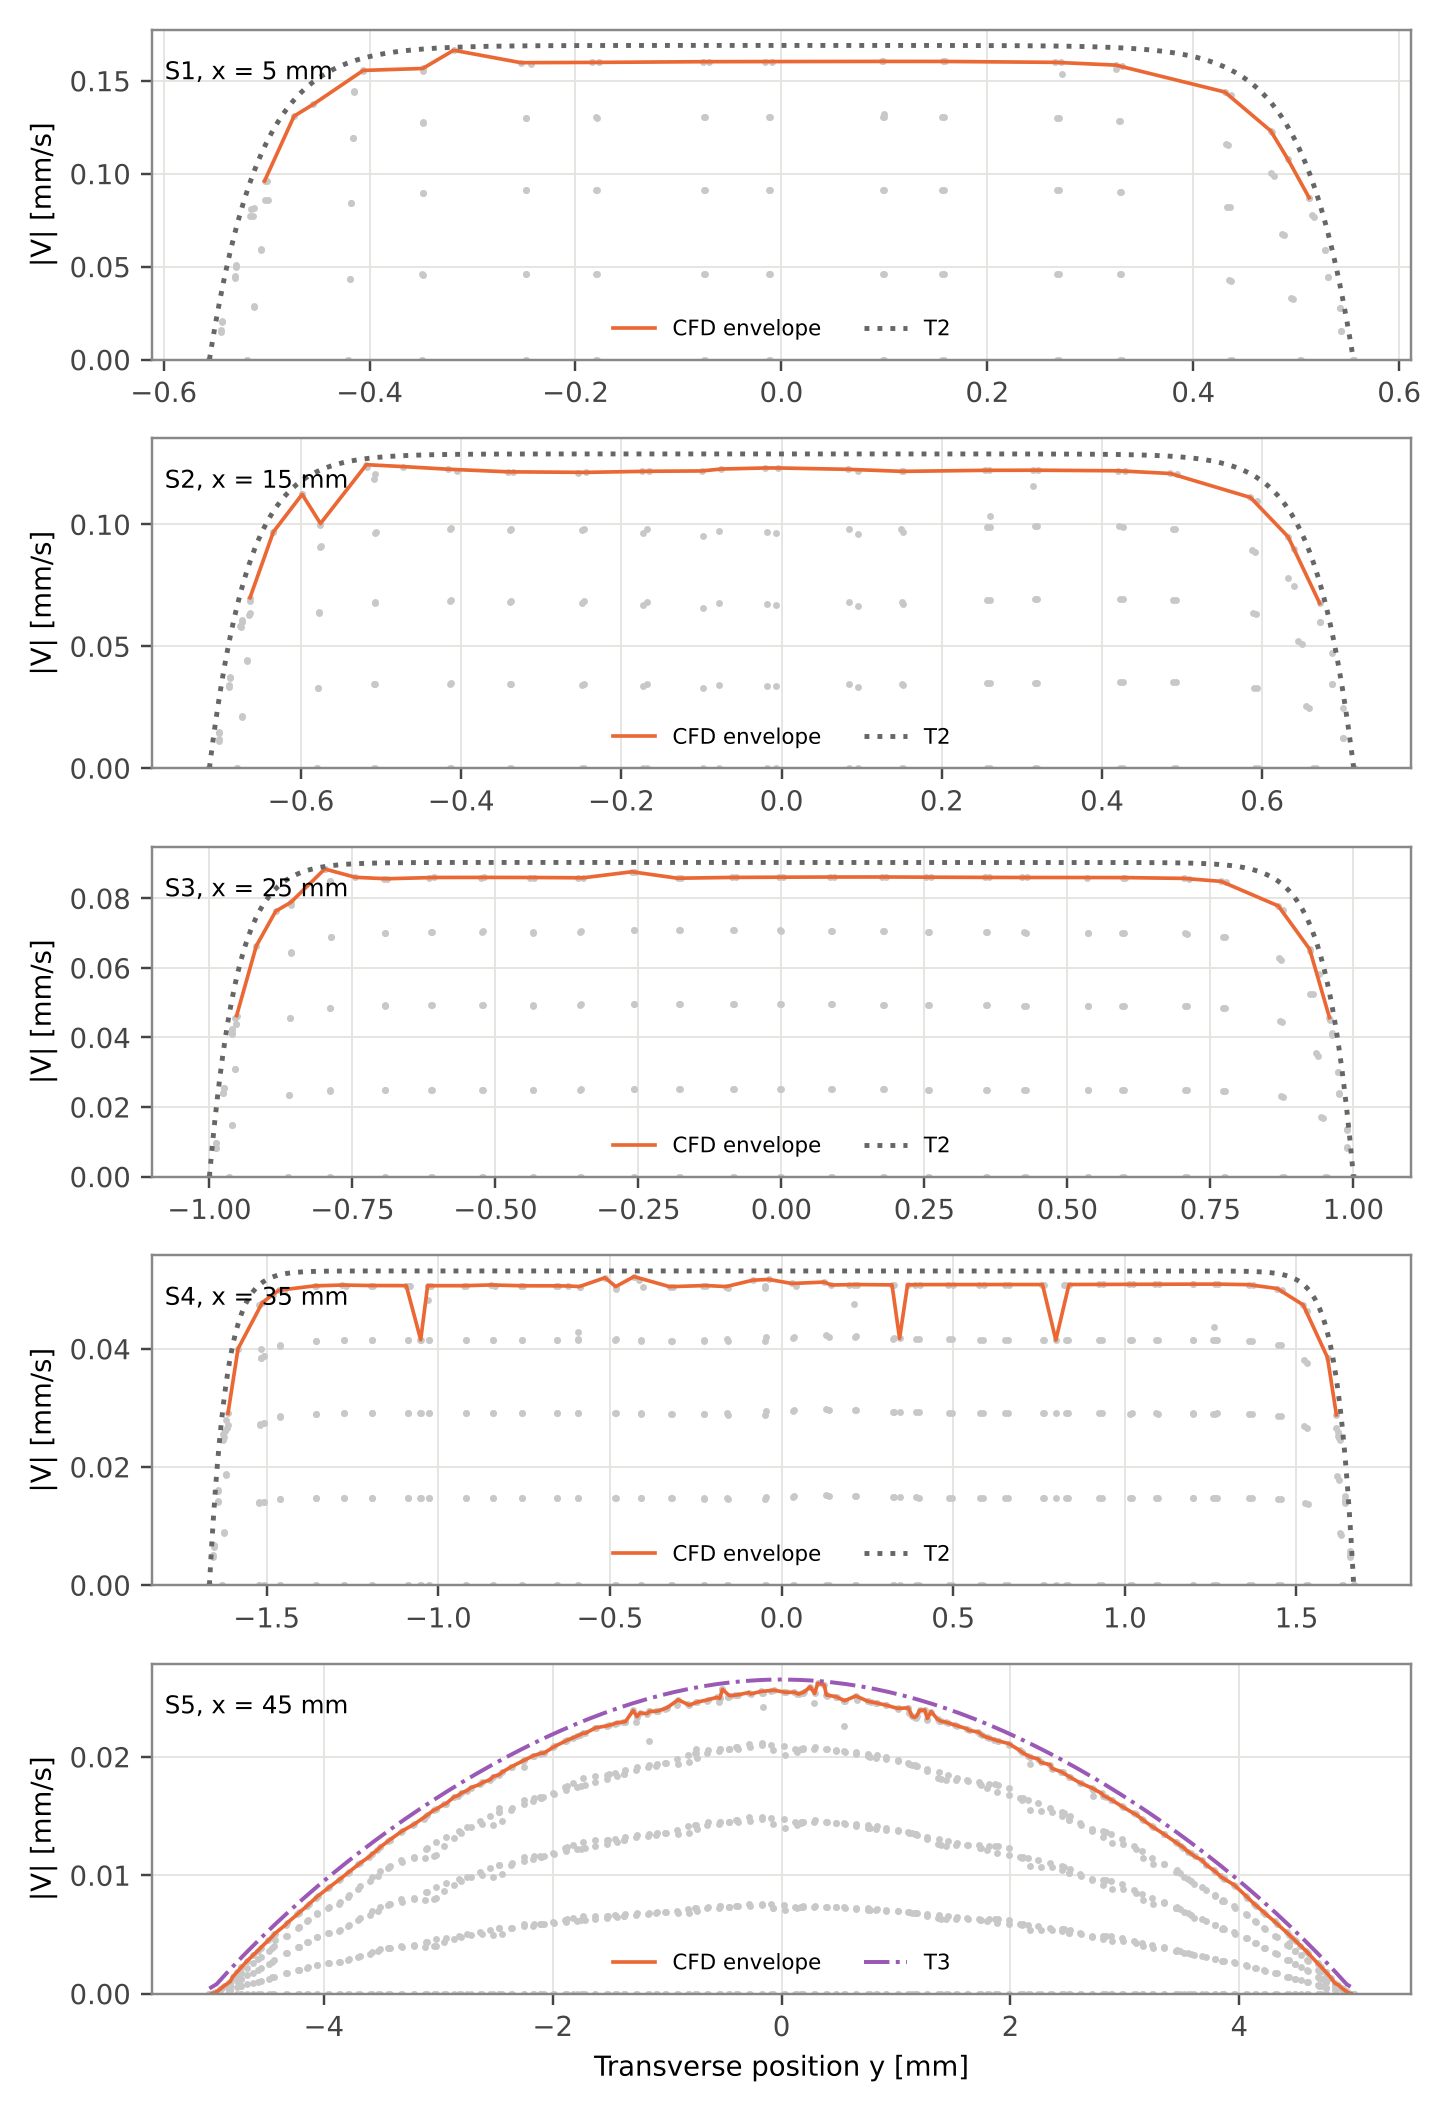
\includegraphics[width=\linewidth]{Fig33_transverse_velocity_all_sections.png}
\caption{Velocity magnitude across the width.}
\end{subfigure}\hfill
\begin{subfigure}[t]{0.49\linewidth}\centering
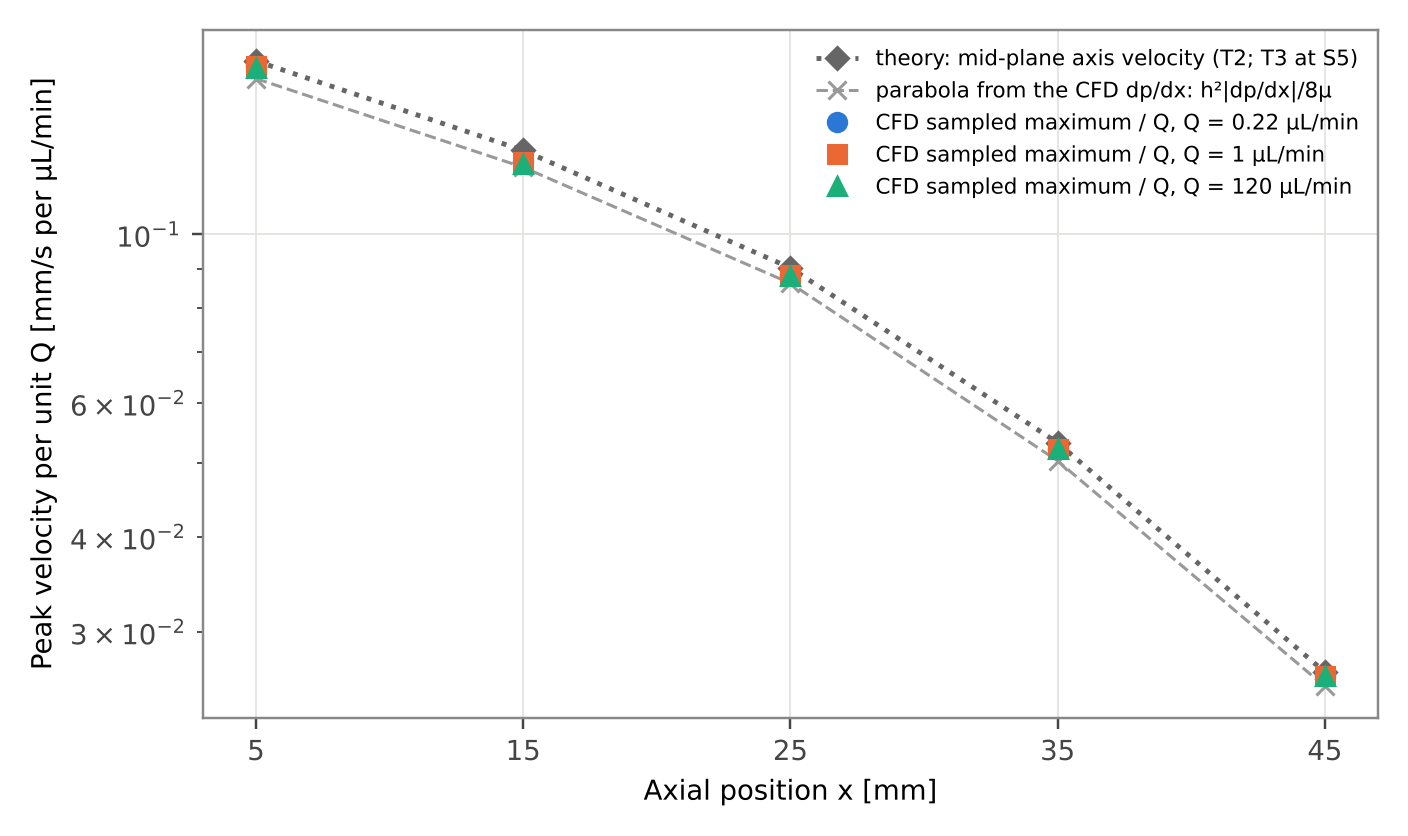
\includegraphics[width=\linewidth]{Fig35_peak_velocity_vs_x.png}
\caption{Peak velocity along the channel.}
\end{subfigure}
\caption{Velocity at the stations \tagC. (a) Nodes at all heights plotted against $y$ (\SI{1}{\uLmin}). The upper envelope is the near-mid-plane profile: a flat core with side-wall layers. (b) Highest sampled $|\vect u|/Q$ against the theoretical mid-plane maximum (T2 at S1--S4, T3 at S5).}
\label{fig:velocity}
\end{figure}

\begin{figure}[htbp]
\centering
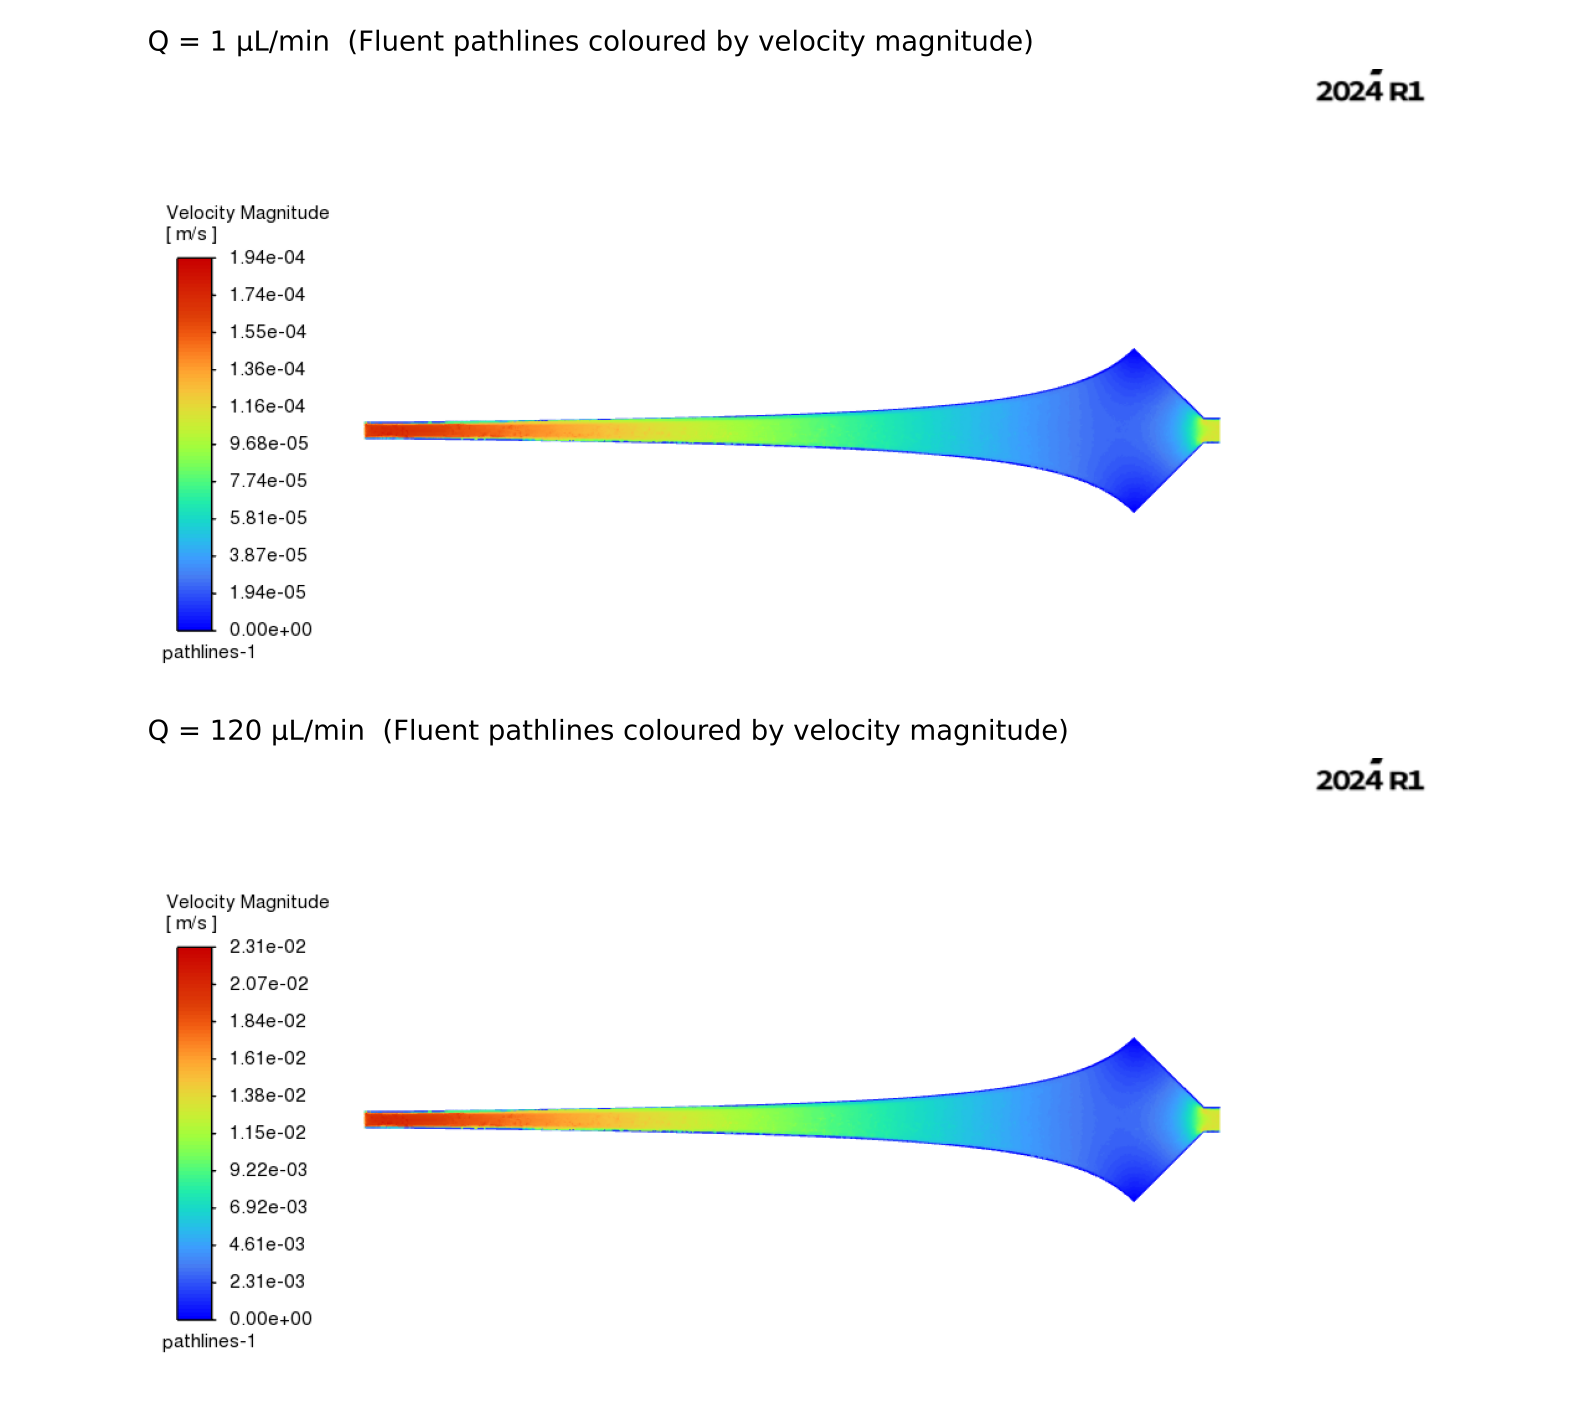
\includegraphics[width=0.75\linewidth]{Fig36_pathlines_Q1_Q120.png}
\caption{Pathlines coloured by velocity magnitude at 1 and \SI{120}{\uLmin} (Fluent images) \tagC. The maximum velocity scales by 119.1 between the two flow rates (Stokes flow: 120). There is no separation or recirculation in the outlet corners.}
\label{fig:pathlines}
\end{figure}

\begin{table}[htbp]
\centering
\caption{Velocity at the stations, \SI{1}{\uLmin}. Theory: T2 mid-plane axis value at S1--S4, T3 at S5. The last column compares the sampled maximum with the parabola implied by the CFD's own pressure gradient, $h^2|\dd p/\dd x|/8\mu$ (\cref{eq:th_umax}).}
\label{tab:velocity}
\small
\begin{tabular}{@{}lccccc@{}}
\toprule
Station & Wall half-angle & Max.\ sampled $|\vect u|$ & Theory mid-plane & Max / theory & Max / $\frac{h^2|\dd p/\dd x|}{8\mu}$\\
 & & [mm/s] & [mm/s] & & \\
\midrule
S1 & \ang{0.71} & 0.1664 & 0.1690 & 0.985 & 1.039\\
S2 & \ang{1.17} & 0.1245 & 0.1289 & 0.966 & 1.016\\
S3 & \ang{2.29} & 0.0884 & 0.0903 & 0.979 & 1.026\\
S4 & \ang{6.34} & 0.0522 & 0.0532 & 0.982 & 1.038\\
S5 & \ang{45} & 0.0262 & 0.0265 & 0.988 & 1.032\\
\bottomrule
\end{tabular}
\end{table}

\section{Cross-comparisons: momentum balance and offset-free ratios}
\label{sec:val_cross}

\paragraph{Momentum balance.} For a locally parabolic flow, the floor shear and the pressure gradient on the axis are linked by $\taw=(h/2)|\dd p/\dd x|$ (\cref{eq:th_tauw}), independently of any theory of the planform. Applied to the two exported CFD fields, this balance holds to within \SI{0.8}{\percent} at all stations and all flow rates, including S5 (\cref{tab:momentum}, \cref{fig:momentum}). The two exports are thus physically consistent with each other. Solved for $h$, the balance gives 143.9--\SI{145.8}{\micro\metre}, which supports the assumed \SI{145}{\micro\metre}.

\begin{table}[htbp]
\centering
\caption{Momentum balance on the axis: CFD wall shear against $(h/2)|\dd p/\dd x|$ from the CFD pressure \tagC.}
\label{tab:momentum}
\small
\begin{tabular}{@{}lcccccc@{}}
\toprule
Station & $\taw$ CFD & $(h/2)|\dd p/\dd x|$ & Ratio & Ratio & Ratio & Implied $h$\\
 & [mPa] & [mPa] & (0.22) & (1) & (120) & [\si{\micro\metre}]\\
\midrule
S1 & 4.1537 & 4.1557 & 0.9995 & 0.9995 & 1.0005 & 144.9\\
S2 & 3.1516 & 3.1764 & 0.9922 & 0.9922 & 0.9926 & 143.9\\
S3 & 2.2303 & 2.2352 & 0.9978 & 0.9978 & 0.9984 & 144.7\\
S4 & 1.3125 & 1.3050 & 1.0057 & 1.0057 & 1.0063 & 145.8\\
S5 & 0.6547 & 0.6589 & 0.9937 & 0.9936 & 0.9932 & 144.1\\
\bottomrule
\end{tabular}
\end{table}

\paragraph{Offset-free comparison.} A ratio of the same quantity at two positions cancels any uniform offset. The axial shape of the shear, expressed relative to S3, agrees with T3 to within \SI{1}{\percent} at every station, \emph{including S5}, whereas Eq.~2 errs by \SI{+3.5}{\percent} at S1 and \SI{+47}{\percent} at S5 (\cref{tab:offset_free}). The normalised pressure $p(x)/p(0)$ agrees with T3 to within \SI{0.08}{\percent} of $p(0)$ over the whole domain, and $p_{\mathrm{CFD}}/p_{T3}=0.950\pm0.001$ along 0--\SI{49.5}{mm}. To a very good approximation, the CFD field is the T3 field multiplied by 0.95.

\begin{table}[htbp]
\centering
\caption{Offset-free comparisons with T3 and Eq.~2, \SI{1}{\uLmin}.}
\label{tab:offset_free}
\small
\begin{tabular}{@{}lccccc@{}}
\toprule
Quantity & CFD & T3 & Eq.~2 & CFD vs T3 [\%] & CFD vs Eq.~2 [\%]\\
\midrule
$\taw(\mathrm{S1})/\taw(\mathrm{S3})$ & 1.8624 & 1.8718 & 1.8000 & $-0.50$ & $+3.46$\\
$\taw(\mathrm{S2})/\taw(\mathrm{S3})$ & 1.4130 & 1.4274 & 1.4000 & $-1.00$ & $+0.93$\\
$\taw(\mathrm{S4})/\taw(\mathrm{S3})$ & 0.5885 & 0.5887 & 0.6000 & $-0.04$ & $-1.92$\\
$\taw(\mathrm{S5})/\taw(\mathrm{S3})$ & 0.2935 & 0.2939 & 0.2000 & $-0.12$ & $+46.77$\\
$p_{\mathrm{CFD}}/p_{T3}$, 0--\SI{49.5}{mm} & \multicolumn{2}{c}{$0.9498\pm0.0010$} & -- & $-5.02$ & --\\
\bottomrule
\end{tabular}
\end{table}

\begin{figure}[htbp]
\centering
\begin{subfigure}[t]{0.49\linewidth}\centering
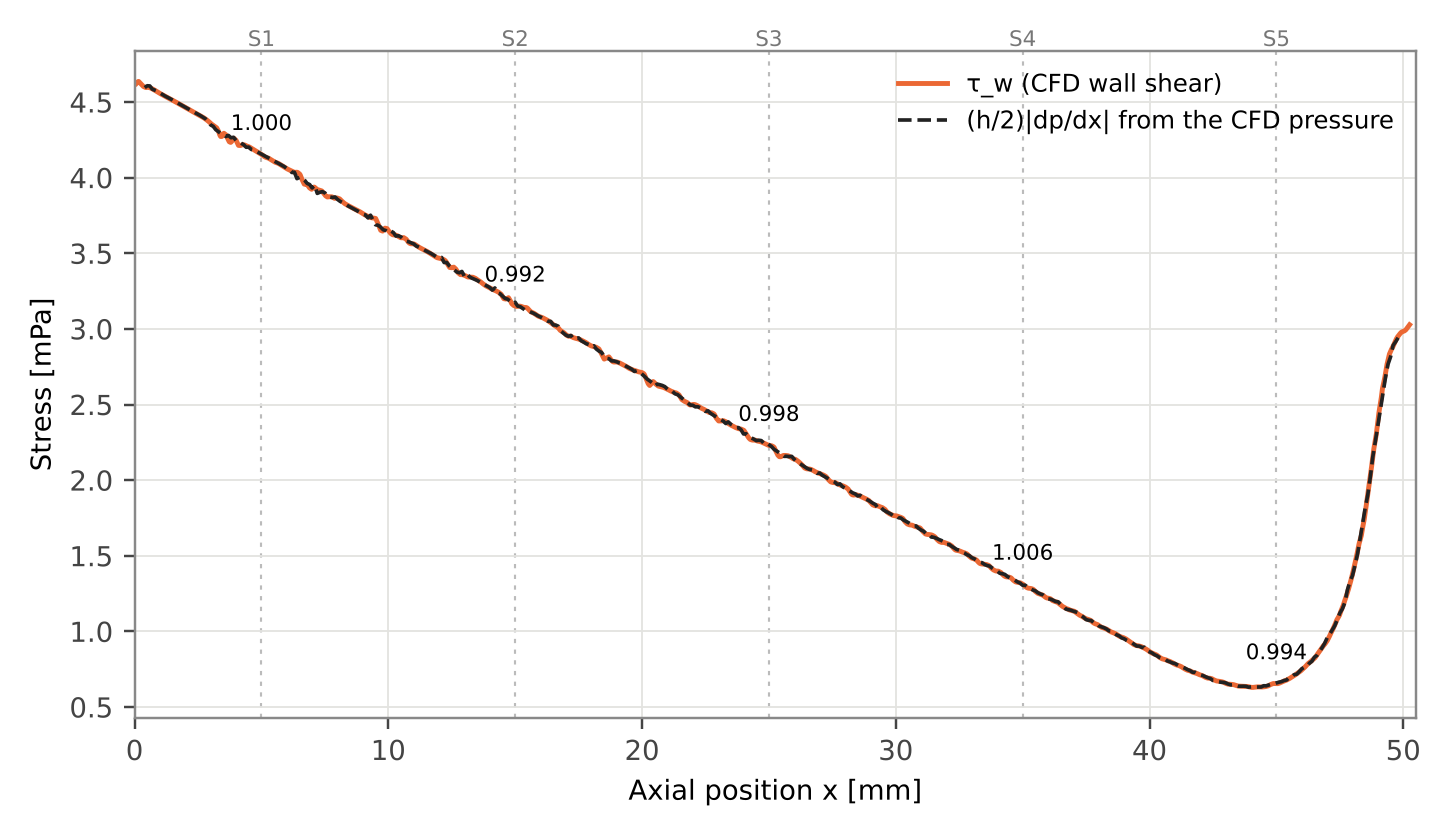
\includegraphics[width=\linewidth]{Fig38_pressure_gradient_vs_shear.png}
\caption{Momentum balance on the axis.}\label{fig:momentum}
\end{subfigure}\hfill
\begin{subfigure}[t]{0.49\linewidth}\centering
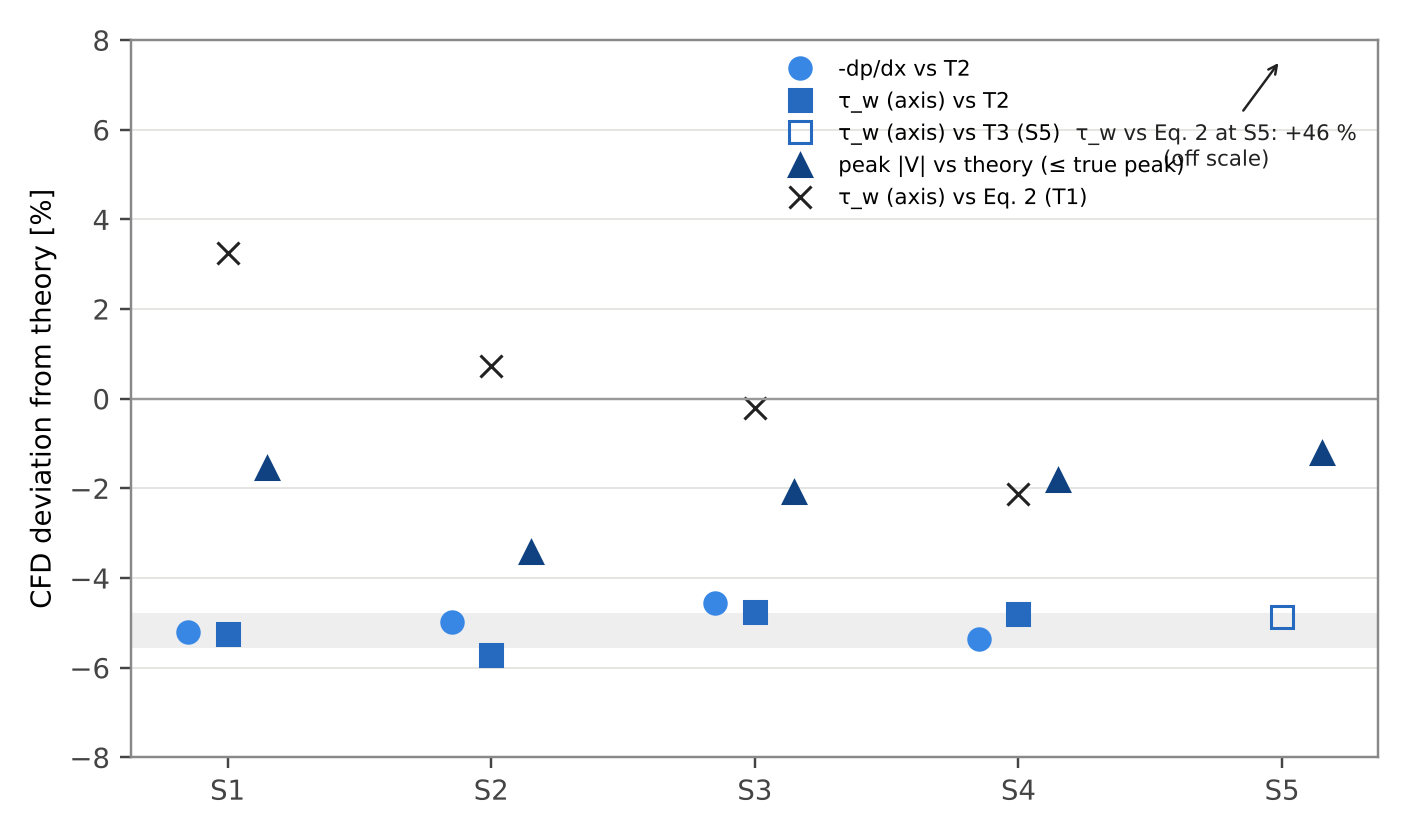
\includegraphics[width=\linewidth]{Fig37_validation_ratios_by_station.png}
\caption{Deviation from the best applicable theory.}\label{fig:val_ratios}
\end{subfigure}
\caption{(a) CFD wall shear against $(h/2)|\dd p/\dd x|$ from the CFD pressure; labels are the ratios \tagC. (b) Deviation of the CFD pressure gradient, wall shear and peak velocity from T2 (S1--S4) or T3 (S5); crosses mark Eq.~2. Pressure gradient and shear are uniformly about \SI{5}{\percent} low (grey band = mean $\pm$ s.d.\ over 2--\SI{40}{mm}); the peak velocity is within \SI{3.5}{\percent}. The S5 point against Eq.~2 (\SI{+46}{\percent}) is off-scale.}
\end{figure}

\section{Origin of the \texorpdfstring{\SI{-5}{\percent}}{-5 \%} offset}
\label{sec:val_offset}

Pressure gradient and wall shear are \SI{5.2(4)}{\percent} below the side-wall-corrected theory, uniformly in $x$ and identically at all three flow rates. Three causes are possible.
\begin{enumerate}
\item \textbf{Discretisation error across the gap (most likely).} About nine cell layers span $h$ everywhere, so an error caused by the wall-normal resolution has the same relative size at every station, as observed. Under-resolving the near-wall velocity gradient lowers the computed wall friction, and with it both the wall shear and the pressure gradient. These two stay mutually consistent (\cref{tab:momentum}). The decisive evidence is the velocity. The CFD peak velocity is \SIrange{1.6}{3.9}{\percent} \emph{higher} than $h^2|\dd p/\dd x|/8\mu$ (\cref{tab:velocity}, last column), which is the largest velocity that an exact parabolic profile with the CFD's own gradient can reach. Exceeding it is the signature of a discrete profile with too little wall friction.
\item \textbf{Flow deficit or incomplete convergence (less likely as the only cause).} A \SI{5}{\percent} lower flow rate would lower $p$, $\taw$ and $u$ by the same \SI{5}{\percent}. The peak velocity is, however, only 1.2--\SI{3.4}{\percent} below theory, and it is itself a lower bound because the sampled nodes are not exactly at mid-height. The missing mass-flux report means this cause cannot be fully excluded.
\item \textbf{A different channel height (unlikely).} A taller channel lowers $\Delta p\propto h^{-3}$, $\taw\propto h^{-2}$ and $u\propto h^{-1}$ by different amounts. No single $h$ can produce equal offsets in pressure gradient and shear, and the momentum balance gives $h=\SI{145(1)}{\micro\metre}$.
\end{enumerate}
The absolute CFD shear values should therefore be quoted as probably about \SI{5}{\percent} low until the mesh study of \cref{sec:num_gci} has been performed.

\section{Flow-rate scaling and regional behaviour}
\label{sec:val_scaling}

All interior quantities are proportional to $Q$ to within \SI{0.08}{\percent} (\cref{fig:scaling}a). The 0.22 and \SI{1}{\uLmin} cases agree to within \SI{0.001}{\percent}. At \SI{120}{\uLmin} ($\Rey_{D_h}=3.65$) the largest departures are \SI{+0.68}{\percent} for the shear peak at the inlet face and \SI{-0.8}{\percent} for the maximum velocity in the pathline images. Inertia therefore matters only at the inlet face of the lead-in, outside the measurement section, which confirms the Stokes-flow estimate of \cref{sec:dimensionless}.

\begin{figure}[htbp]
\centering
\begin{subfigure}[t]{0.49\linewidth}\centering
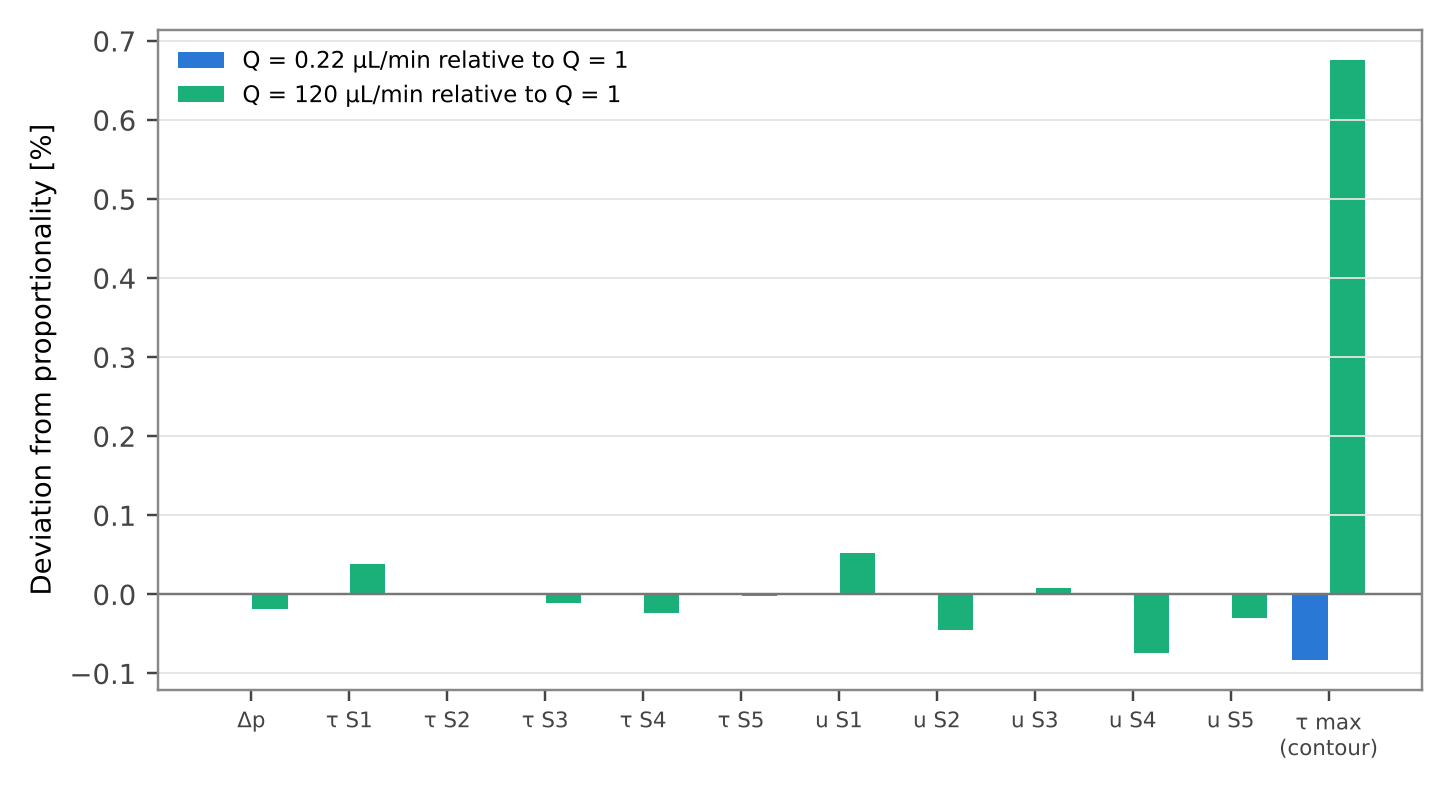
\includegraphics[width=\linewidth]{Fig40_flow_rate_scaling.png}
\caption{Departure from proportionality with $Q$.}
\end{subfigure}\hfill
\begin{subfigure}[t]{0.49\linewidth}\centering
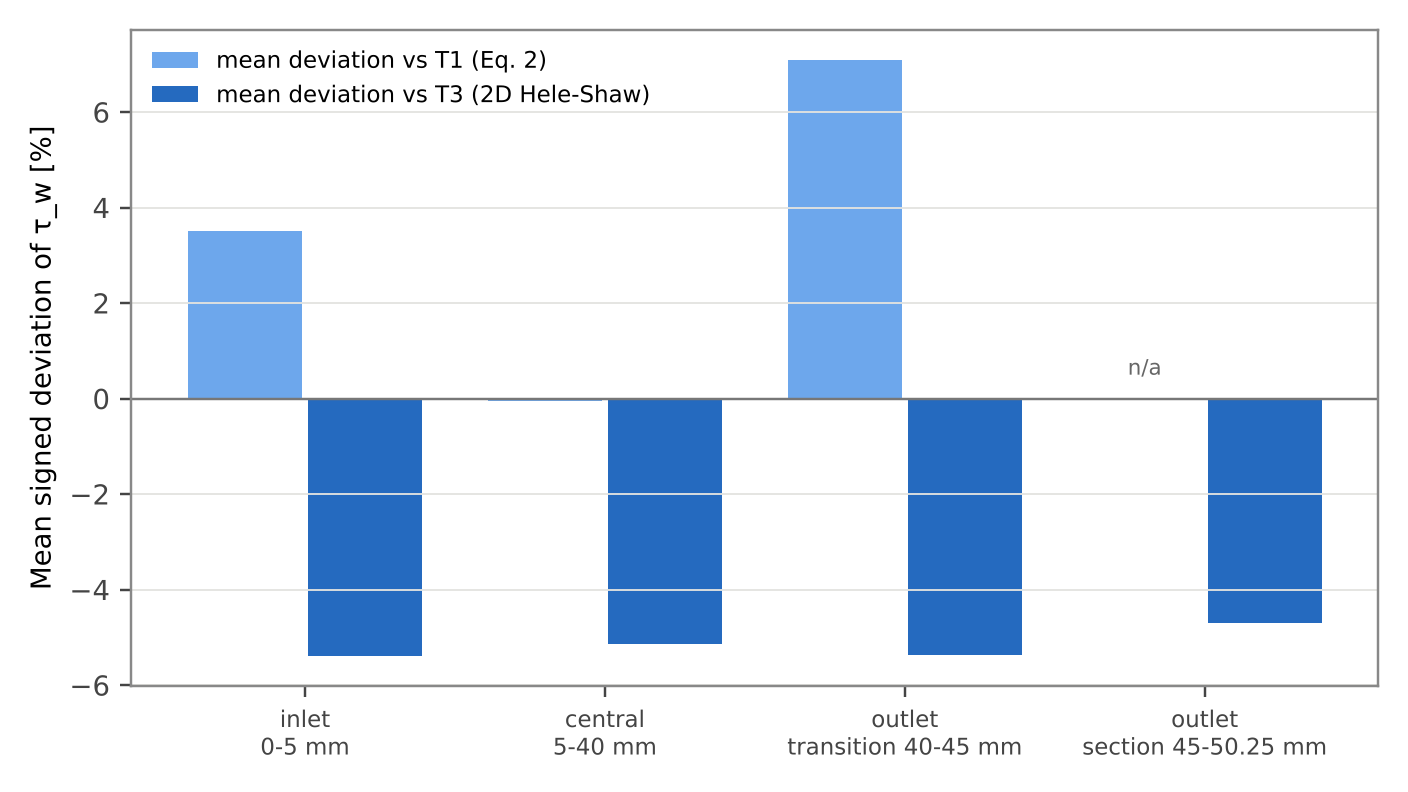
\includegraphics[width=\linewidth]{Fig41_regional_deviation.png}
\caption{Regional deviation of the axial shear.}
\end{subfigure}
\caption{(a) Percentage departure of each quantity from exact proportionality with $Q$, relative to \SI{1}{\uLmin} \tagC. (b) Mean signed deviation of the axial shear from Eq.~2, T2 and T3 in four regions (\SI{1}{\uLmin}). Eq.~2 is accurate on average in the central region but fails in the outlet transition; T3 removes the regional dependence and leaves the uniform \SI{-5}{\percent} offset.}
\label{fig:scaling}
\end{figure}

The regional analysis (\cref{fig:scaling}b) gives the following picture. In the inlet region (0--\SI{5}{mm}), the CFD exceeds Eq.~2 by \SI{3.5}{\percent} on average. In the central region (5--\SI{40}{mm}), the mean deviation is \SI{-0.05}{\percent}, although it ranges from \SI{+3.8}{\percent} to \SI{-3.1}{\percent} along $x$. In the outlet transition (40--\SI{45}{mm}), the mean deviation is \SI{+7.1}{\percent} and reaches \SI{+45}{\percent} at $x=\SI{45}{mm}$. Against T3 the mean deviation is between $-5.4$ and \SI{-4.7}{\percent} in every region.

\section{Physical interpretation of the flow field}
\label{sec:val_physics}

\paragraph{Velocity and flow distribution.} The flow is a Stokes flow in which each vertical column of fluid balances the local pressure gradient against the friction of the floor and the lid. The velocity profile across the gap is parabolic, and across the width it is flat except within about one gap height of the side walls. As the channel widens, the same flow is spread over a wider section, so the velocity falls as $1/w$, from \SI{0.17}{mm/s} at S1 to \SI{0.026}{mm/s} at S5 at \SI{1}{\uLmin}.

\paragraph{Pressure distribution and losses.} Since $\dd p/\dd x\propto1/w$, the pressure is lost mainly in the narrow upstream part: \SI{52}{\percent} of the T1 drop over the hyperbolic section occurs in its first \SI{15}{mm}, one third of its length. The resistance is linear, $R_{\mathrm{hyd}}=\SI{9.94e10}{Pa.s/m^3}$ from $x=0$ to the outlet, as expected for Stokes flow. The pressure drop of \SI{1.66}{Pa} at \SI{1}{\uLmin} is negligible for any syringe pump, but the corresponding velocities are very small. This becomes important for oxygen (\cref{ch:o2results}).

\paragraph{Wall shear.} The shear is set by the local pressure gradient, $\taw=(h/2)|\dd p/\dd x|$, and therefore falls as $1/w(x)$, i.e.\ linearly in $x$. Two effects modify this design behaviour. First, the side walls carry part of the drag, so for a given $Q$ a larger pressure gradient is needed, which raises the floor shear on the axis by $0.63\,h/w$. This is \SI{9}{\percent} at S1 and decreases downstream. Second, the converging outlet makes the flow two-dimensional within about \SI{3}{mm} of the corner: the iso-bars curve, the flow along the axis accelerates towards the outlet, and the shear passes through a minimum at \SI{44}{mm} and rises again. S5 lies exactly on this corner.

\paragraph{Development of the velocity profile.} The parabolic profile is established within $\sim\SI{0.09}{mm}$ of the inlet face and adapts instantly to the slow changes of width ($\Rey^*\ll1$). The flow is therefore locally fully developed everywhere in the hyperbolic section. There is no entrance effect at $x=0$ beyond a \SI{0.5}{\percent} local shear excess at $x\approx\SI{0.16}{mm}$, where the wall slope changes from zero (lead-in) to that of the hyperbola.

\paragraph{Local variations across the width.} The side-wall layer has a fixed thickness of about $0.9h$. Its share of the width shrinks downstream, so the region of uniform shear grows from \SI{70}{\percent} to \SI{91}{\percent} of the width between S1 and S4. This favours imaging in the downstream sections, up to the point where the outlet corner takes over.

\section{Validation summary}

\Cref{tab:validation_matrix} classifies each comparison.

\begin{table}[htbp]
\centering
\caption{Validation summary (\SI{1}{\uLmin}; other flow rates within \SI{0.1}{\percent}).}
\label{tab:validation_matrix}
\scriptsize
\begin{tabularx}{\linewidth}{@{}p{0.2\linewidth}p{0.22\linewidth}p{0.22\linewidth}X@{}}
\toprule
Quantity & Expectation & Observation & Classification and reason\\
\midrule
Published shear range \tagP & 0.01--0.001 and 0.0447--\SI{0.0059}{\dyncm} & 0.0102--0.0014 and 0.0464--\SI{0.0063}{\dyncm} & \textbf{Consistent} (semi-quantitative; published curves not tabulated)\\
Published imaging zone \tagP & $D_{\max}$ 0.34--\SI{3.84}{mm} & S3--S4 within \SI{2}{\percent}; S1--S2 +15 to \SI{+17}{\percent}; S5 differs & \textbf{Partly consistent}; criterion not stated in paper\\
Shape of $p(x)$ & T3 & $p/p(0)$ within \SI{0.08}{\percent} of T3 & \textbf{Quantitatively validated}\\
Magnitude of $\Delta p$ & T2/T3 & \SI{-4.9}{\percent} / \SI{-5.2}{\percent} & \textbf{Deviating} (uniform offset)\\
$\taw$ vs Eq.~2, S1--S4 & T1 & $+3.2$, $+0.7$, $-0.2$, \SI{-2.1}{\percent} & \textbf{Consistent}, but partly a cancellation of errors\\
Side-wall effect on $\taw$ & $1/f-1\approx0.63\,h/w$ & correct slope, offset \SI{-4.9}{\percent} & \textbf{Quantitatively validated} (slope)\\
Axial shape of $\taw$ & T3 ratios & within \SI{1}{\percent}, incl.\ S5 & \textbf{Quantitatively validated}\\
$\taw$ at S5 & T3: \SI{+54}{\percent} vs Eq.~2 & \SI{+46.5}{\percent} vs Eq.~2 & \textbf{Consistent}; Eq.~2 invalid at S5\\
Side-wall layer, uniform zone & \SI{0.129}{mm}; $d=w/2-0.129$ & 0.15--\SI{0.17}{mm}; $d$ 0.01--\SI{0.03}{mm} smaller & \textbf{Consistent} within node spacing\\
Transverse profile at S5 & T3 dome, $d=\SI{1.050}{mm}$ & dome, $d=\SI{1.024}{mm}$ & \textbf{Quantitatively validated}\\
Velocity across the width & flat core, side-wall layer & reproduced; peak 1.2--\SI{3.4}{\percent} low & \textbf{Consistent}\\
Velocity across the gap $u(z)$ & parabola & not exported & \textbf{Inconclusive} (no data)\\
Momentum balance & exact & within \SI{0.8}{\percent}; $h=\SI{145(1)}{\micro\metre}$ & \textbf{Quantitatively validated}\\
Peak velocity vs own gradient & $\le h^2|\dd p/\dd x|/8\mu$ & \SIrange{1.6}{3.9}{\percent} above & \textbf{Deviating}: under-resolved gap\\
Linearity in $Q$ & exact (Stokes) & within \SI{0.08}{\percent} & \textbf{Quantitatively validated}\\
Mesh independence & GCI from 3 meshes & one mesh only & \textbf{Inconclusive} (study pending)\\
\bottomrule
\end{tabularx}
\end{table}

\begin{keybox}[Answer to RQ1--RQ3]
The CFD reproduces every shape that the theory predicts: the axial distributions of pressure and shear (within \SI{1}{\percent}), the side-wall correction to Eq.~2 (with the correct slope), the side-wall layer, the dome-shaped profile at S5 and exact Stokes scaling. It also reproduces the published shear ranges and the published imaging zones at S3--S4. It does not yet reproduce the absolute magnitude: shear and pressure gradient are uniformly about \SI{5}{\percent} below the theory that includes side-wall drag, most probably because there are too few cells across the gap. Eq.~2 itself is accurate to $\pm\SI{4}{\percent}$ for $0\le x\lesssim\SI{40}{mm}$ only because the side-wall drag it omits and the CFD offset partly cancel. Eq.~2 fails at S5.
\end{keybox}

\chapter{Motivation and Development of the Oxygen Transport Model}
\label{ch:o2motivation}

\section{Why oxygen matters in this device}

Aerobic cells use oxygen continuously. Their uptake rate spans more than two orders of magnitude between cell types, from below 1 to more than \SI{350}{amol} per cell per second \citep{Wagner2011}. Oxygen is poorly soluble in water: air-saturated culture medium at \SI{37}{\celsius} holds only about \SI{0.18}{mol/m^3} \citep{Wenger2015}. A monolayer can therefore deplete the medium above it quickly unless the medium is renewed. In static culture this is a known, often unmeasured, limitation \citep{Place2017}. Even in Caco-2 cultures, which rely largely on glycolysis, the pericellular oxygen level depends on cell density and on the height of the medium \citep{Zeitouni2015}.

In organ-on-chip devices, flow renews the medium, but the flow rates that give physiologically low shear also deliver little oxygen. The widening Hele-Shaw chip is an extreme case. It is designed to reach very low shear (down to \SI{e-3}{\dyncm}) at flow rates of a fraction of a \ulmin, and the lowest shear occurs in the widest, downstream part of the channel, which receives medium that has already passed over the upstream cells. The same geometric feature that creates the shear gradient may therefore create an oxygen gradient in the same direction. If it does, a biological response attributed to low shear could in fact be a response to low oxygen. PDMS is permeable to oxygen and can supply it through the walls. Measurements in perfused PDMS bioreactors nevertheless show that cell uptake can produce axial oxygen gradients despite this permeability \citep{Mehta2007}.

The flow solution of Part A gives the shear field but says nothing about oxygen. Whether a cell at a given position is well supplied depends on three things together:
\begin{itemize}
\item how much oxygen the flow brings to that position (convection);
\item how fast it crosses the gap to the floor (diffusion);
\item how much the upstream cells have already removed (consumption).
\end{itemize}
A transport model is needed, and the validated flow field is its input.

\section{The physical problem}

\begin{description}[leftmargin=0pt]
\item[Where oxygen enters.] Medium equilibrated with the incubator atmosphere enters at the inlet. The reference protocol keeps the medium reservoir and tubing inside the incubator \citep{Delon2020}. If the lid and side walls are gas-permeable, oxygen also enters through the PDMS from the incubator air.
\item[Where it is transported.] Oxygen is carried along the channel by the flow and diffuses across the gap. Axial diffusion is negligible compared with convection, as shown below.
\item[Where it is consumed.] Oxygen is consumed only by the cell monolayer on the glass floor ($z=0$). The medium itself does not consume oxygen.
\item[Role of diffusion.] Diffusion across the \SI{145}{\micro\metre} gap carries oxygen from the bulk to the cells, and from the lid into the bulk. Its time scale ($\sim\SI{7}{s}$) is short compared with the residence time, so the concentration across the gap is nearly uniform.
\item[Role of convection.] Convection replaces the medium that the cells deplete. Its capacity, $Q\Csat$, is proportional to the flow rate and therefore to the shear.
\item[Included.] The model includes steady convection--diffusion with the validated, frozen velocity field, Michaelis--Menten uptake by the monolayer, and three wall conditions (impermeable, PDMS, saturated).
\item[Neglected.] The model neglects transient re-oxygenation after medium changes, the oxygen transport inside the PDMS (only its steady resistance is kept), cell growth, cell-to-cell variation of uptake, the geometric effect of the cells on the flow, oxygen partitioning at the PDMS--medium interface, and the ports and tubing.
\end{description}

\section{Strategy}

The oxygen problem is developed in the same way as the flow problem. \Cref{ch:o2equations} starts from the general species balance and reduces it with explicit, quantified assumptions. \Cref{ch:o2analytical} derives closed-form solutions for the cases that admit them, and a reduced-order (``1.5-D'') model for the general Michaelis--Menten case; the closed forms provide a check on the reduced-order model. \Cref{ch:o2results} applies both to the three flow rates and the three wall conditions, and discusses what they imply for the device.

\chapter{Governing Equations for Oxygen Transport}
\label{ch:o2equations}

\section{Species conservation equation}

Let $C(\vect x,t)$ be the molar concentration of dissolved oxygen. A balance on a fixed control volume, with the molar flux $\vect J=C\vect u-D\nabla C$ (convection plus Fickian diffusion \citep{BSL2002,Deen2012}), gives
\begin{equation}
\underbrace{\frac{\partial C}{\partial t}}_{\text{accumulation}}
+\underbrace{\nabla\cdot(\vect uC)}_{\text{convection}}
=\underbrace{\nabla\cdot(D\nabla C)}_{\text{diffusion}}
+\underbrace{R}_{\text{volumetric production}} .
\label{eq:ox_general}
\end{equation}
\begin{itemize}
\item The accumulation term is the rate of change of oxygen stored in a unit volume.
\item The convective term is the net outflow of oxygen carried by the medium.
\item The diffusive term is the net inflow by molecular diffusion down concentration gradients, with diffusivity $D$.
\item $R$ (\si{mol.m^{-3}.s^{-1}}) is the production rate per unit volume; consumption is negative.
\end{itemize}

\section{Simplification of the governing equation}

Each assumption below is checked against the actual parameters (\cref{tab:o2params}). The list states whether an assumption is \emph{used} in the model or is only an alternative.

\begin{enumerate}
\item \textbf{Dilute solution} (used). The oxygen mass fraction is $Y=CM_{\mathrm{O_2}}/\rho=0.178\times0.032/981.8\approx\num{5.8e-6}$. Oxygen therefore has no effect on the density or viscosity of the medium, and Fick's law for a dilute binary mixture applies.
\item \textbf{Constant diffusivity} (used). The system is isothermal at \SI{37}{\celsius}, so $D=\SI{3.0e-9}{m^2/s}$ \citep{HanBartels1996}, with a sensitivity range of 2.6--\SI{3.3e-9}{m^2/s}. Then $\nabla\cdot(D\nabla C)=D\nabla^2C$.
\item \textbf{Incompressible flow} (used). Since $\nabla\cdot\vect u=0$ (\cref{eq:gov_cont}), $\nabla\cdot(\vect uC)=\vect u\cdot\nabla C$.
\item \textbf{One-way coupling} (used). Oxygen does not affect the flow (point 1), so the velocity field of Part A is prescribed (``frozen'').
\item \textbf{No reaction in the medium} (used). The medium does not consume oxygen, so $R=0$ in the fluid.
\item \textbf{Uptake as a surface flux} (used). A confluent monolayer is about 5--\SI{10}{\micro\metre} thick, much thinner than the gap. The oxygen drop that diffusion through a layer of thickness $\delta_c$ needs to supply the uptake is of order $\qmax\delta_c/D$, i.e.\ a fraction $\Da_w\,\delta_c/h\approx10^{-3}$ of $\Csat$ (with $\Da_w$ defined in \cref{tab:o2groups}). The monolayer can therefore be represented by a boundary flux on the floor. The alternative, a volumetric sink in a layer of thickness $\delta_c$, gives the same result to this accuracy and would require meshing the cell layer.
\item \textbf{Steady state} (used). Three time scales are relevant:
\begin{itemize}
\item diffusion across the gap, $t_D=h^2/D=\SI{7.0}{s}$;
\item residence in the cell-culture section, $t_{\mathrm{res}}=A_{\mathrm{cells}}h/Q=\SI{4553}{s}$, \SI{1002}{s} and \SI{8.3}{s} at 0.22, 1 and \SI{120}{\uLmin};
\item equilibration of the \SI{5}{mm} PDMS lid, of order hours.
\end{itemize}
Cultures last days (5 days to confluence in the reference protocol \citep{Delon2020}), so the steady state is the relevant one. Transients after a medium change or a change of flow rate last up to about 1--\SI{2}{h}, and are outside the scope of this report.
\item \textbf{Uptake kinetics} (Michaelis--Menten used; zero order used for closed forms). Three standard forms are considered:
\begin{equation}
q=\begin{cases}
\qmax & \text{zero order},\\[2pt]
\dfrac{\qmax}{\Km}\,C & \text{first order},\\[6pt]
\qmax\dfrac{C}{\Km+C} & \text{Michaelis--Menten}.
\end{cases}
\label{eq:ox_kinetics}
\end{equation}
Michaelis--Menten kinetics reduces to zero order for $C\gg\Km$ and to first order for $C\ll\Km$. With $\Csat/\Km=283$, the uptake stays within \SI{10}{\percent} of $\qmax$ until $C$ falls below $9\Km\approx0.03\,\Csat$. The zero-order closed forms are therefore accurate wherever the cells are not already close to anoxia. First-order kinetics alone would grossly under-predict the uptake at normal concentrations, so it is used only in the analysis near anoxia.
\end{enumerate}

With these assumptions \cref{eq:ox_general} becomes the steady convection--diffusion equation with a prescribed velocity field,
\begin{equation}
\vect u\cdot\nabla C=D\nabla^2C\qquad\text{in the fluid},
\label{eq:ox_cd}
\end{equation}
and all consumption enters through the boundary condition on the floor.

\section{Coupling with the flow field}

The velocity in \cref{eq:ox_cd} is the steady field validated in \cref{ch:validation}. Two levels of coupling are possible.
\begin{enumerate}
\item \textbf{CFD (planned).} Solve \cref{eq:ox_cd} in Fluent as a user-defined scalar (UDS) on the converged, frozen velocity field, with a user-defined function (UDF) for the Michaelis--Menten wall flux and for the PDMS Robin condition. This set-up has been prepared but not yet run. It would resolve the side-wall layers and the outlet corner.
\item \textbf{Reduced-order model (used here).} Represent the velocity by the lubrication solution validated in Part A: the profile across the gap is parabolic and the flow rate is $Q$ through every section. The oxygen balance then depends only on $Q$, $h$ and $w(x)$. It does not depend on the absolute magnitude of the CFD shear, so the \SI{-5}{\percent} offset of \cref{sec:val_offset} does not affect it.
\end{enumerate}
Both approaches are one-way coupled. Their main limitation is that the reduced-order model treats the cross-section as uniform across the width. The slower fluid in the side-wall layers (about \SI{0.13}{mm} on each side) has a longer residence time and will be more depleted than the reduced-order model predicts. This is a three-dimensional effect that only the CFD can quantify.

\section{Boundary conditions}

The outward unit normal is $\vect n$. The diffusive flux of oxygen into the fluid through a wall is $D\,\partial C/\partial n_{\mathrm{in}}$, where $n_{\mathrm{in}}$ is the inward normal.

\paragraph{Inlet.} $C=\Csat$. The medium arrives equilibrated with the incubator atmosphere: the reservoir and tubing are in the incubator \citep{Delon2020}, and the lead-in is too short for significant uptake. With $\alpha=1.26~\mu\mathrm{M\,mmHg^{-1}}$ and an oxygen partial pressure of \SI{141}{mmHg} in a humidified \SI{5}{\percent} CO$_2$ incubator \citep{Wenger2015}, $\Csat=\SI{0.178}{mol/m^3}$.

\paragraph{Outlet.} Zero diffusive flux, $\partial C/\partial x=0$. Axial diffusion is negligible ($\Pe_L\ge421$, \cref{tab:o2groups}), so the outlet condition has no influence upstream.

\paragraph{Floor (cells), $z=0$.} The cells remove oxygen at the rate $q$:
\begin{equation}
D\left.\frac{\partial C}{\partial z}\right|_{z=0}=q(\Cbot)=\qmax\frac{\Cbot}{\Km+\Cbot},
\label{eq:ox_bc_floor}
\end{equation}
where $\Cbot$ is the local concentration on the floor. This is a non-linear condition: the uptake decreases smoothly when oxygen runs out, instead of driving $C$ negative as a zero-order flux would.

\paragraph{Lid, $z=h$.} Three cases bracket the real device:
\begin{align}
\text{IMP (impermeable):}&\quad \left.\frac{\partial C}{\partial z}\right|_{z=h}=0, \label{eq:ox_bc_imp}\\
\text{PDMS (Robin):}&\quad D\left.\frac{\partial C}{\partial z}\right|_{z=h}=\kp\,(\Csat-\Ctop), \label{eq:ox_bc_pdms}\\
\text{SAT (saturated):}&\quad C(z=h)=\Csat. \label{eq:ox_bc_sat}
\end{align}
IMP is the worst case and represents glass or thermoplastic chips. SAT is the best case, a lid with no transport resistance.

\paragraph{Derivation of the PDMS coefficient.} At steady state, oxygen diffuses through the lid of thickness $t_{\mathrm{PDMS}}$ from incubator air (partial pressure $p_a$) to the PDMS--medium interface (partial pressure $p_i$). With the permeability $P$ (\si{mol.m^{-1}.s^{-1}.Pa^{-1}}) of PDMS, the flux is $N=P(p_a-p_i)/t_{\mathrm{PDMS}}$. Partial pressure is continuous across the interface, and on the medium side Henry's law gives $p_i=\Ctop/\alpha$ and $p_a=\Csat/\alpha$. Hence
\begin{equation}
\begin{aligned}
N&=\frac{P}{t_{\mathrm{PDMS}}\,\alpha}(\Csat-\Ctop)\equiv\kp(\Csat-\Ctop),\\
\kp&=\frac{\num{2.67e-13}}{\num{5e-3}\times\num{9.45e-6}}=\SI{5.65e-6}{m/s},
\end{aligned}
\label{eq:ox_kpdms}
\end{equation}
using $P=800$ Barrer \citep{Merkel2000}. Formulating the condition in partial pressure avoids the partition coefficient between PDMS and medium. The condition assumes that the outer PDMS surface is exposed to incubator air. The reference protocol mentions immersing the device in water to limit bubbles \citep{Delon2020}; this would add a diffusion resistance and lower $\kp$. Reported reductions of PDMS permeability by protein adsorption \citep{Mehta2007} would do the same.

\paragraph{Side walls.} In the CFD the side walls are PDMS and carry the same condition as the lid. The reduced-order model neglects them. Their area per unit length, $2h$, is \SI{29}{\percent} of the floor width at the inlet and less than \SI{3}{\percent} at S5. Neglecting them is therefore conservative for the PDMS case and exact for IMP.

\section{Parameters and dimensionless groups}

\begin{table}[htbp]
\centering
\caption{Oxygen transport parameters. ``Illustrative'' values are not measured data for Caco-2 or A549 cells and are varied in the sensitivity analysis.}
\label{tab:o2params}
\small
\begin{tabularx}{\linewidth}{@{}p{0.22\linewidth}p{0.17\linewidth}p{0.15\linewidth}X@{}}
\toprule
Parameter & Baseline & Range & Source and status\\
\midrule
$D$, O$_2$ in medium, \SI{37}{\celsius} & \SI{3.0e-9}{m^2/s} & 2.6--\SI{3.3e-9}{} & water value \citep{HanBartels1996}; medium taken as water-like\\
$\Csat$ & \SI{0.178}{mol/m^3} & 0.167--0.200 & $1.26~\mu\mathrm{M\,mmHg^{-1}}\times141~\mathrm{mmHg}$ \citep{Wenger2015}\\
Cell density $\rho_{\mathrm{cell}}$ & \SI{2e9}{m^{-2}} & 1--\SI{5e9}{} & seeding density for Caco-2 \tagP\ \citep{Delon2020}; confluent density is higher\\
OCR per cell & \SI{20}{amol/s} & 5--100 & \textbf{illustrative}; mammalian cells span $<1$ to $>350$ \citep{Wagner2011}\\
$\qmax=\rho_{\mathrm{cell}}\cdot$OCR & \SI{4.0e-8}{mol.m^{-2}.s^{-1}} & 0.5--\SI{50e-8}{} & derived (illustrative)\\
$\Km$ & \SI{6.3e-4}{mol/m^3} (\SI{0.5}{mmHg}) & 0.5--\SI{5}{mmHg} & hepatocyte value \citep{Rotem1994}; not cell-line specific\\
PDMS permeability $P$ & 800 Barrer & 600--800 & \citep{Merkel2000}, \SI{35}{\celsius}\\
PDMS thickness & \SI{5}{mm} & -- & \tagP\ \citep{Delon2020}\\
$\kp$ & \SI{5.65e-6}{m/s} & 0 to $\infty$ & derived, \cref{eq:ox_kpdms}\\
\bottomrule
\end{tabularx}
\end{table}

\begin{table}[htbp]
\centering
\caption{Dimensionless groups and time scales of oxygen transport (baseline parameters; $\bar U_0=Q/(w_1h)$ at the inlet of the hyperbola; $A_{\mathrm{cells}}=\SI{115.13}{mm^2}$) \tagM.}
\label{tab:o2groups}
\small
\resizebox{\linewidth}{!}{%
\begin{tabular}{@{}lp{0.37\linewidth}ccc@{}}
\toprule
Group & Meaning & \SI{0.22}{\uLmin} & \SI{1}{\uLmin} & \SI{120}{\uLmin}\\
\midrule
$\Pe_h=\bar U_0h/D$ & convection along $x$ vs diffusion across $h$ & 1.22 & 5.56 & 667\\
$\Pe_L=\bar U_0L/D$ & axial convection vs axial diffusion & 421 & 1916 & \num{2.3e5}\\
$\Da_w=\qmax h/(D\Csat)$ & uptake vs diffusion across the gap & 0.011 & 0.011 & 0.011\\
$\Da_{\mathrm{conv}}=\qmax A_{\mathrm{cells}}/(Q\Csat)$ & total uptake vs convective supply & \textbf{7.06} & \textbf{1.55} & 0.013\\
$\Bi=\kp h/D$ & lid conductance vs gap conductance & 0.27 & 0.27 & 0.27\\
$\Phi_{\mathrm{PDMS}}=\kp\Csat/\qmax$ & maximum lid supply vs maximum uptake & 25.1 & 25.1 & 25.1\\
$\Csat/\Km$ & saturation of the kinetics & 283 & 283 & 283\\
$t_D=h^2/D$ [s] & diffusion time across the gap & 7.0 & 7.0 & 7.0\\
$t_{\mathrm{res}}=A_{\mathrm{cells}}h/Q$ [s] & residence time in the culture section & 4553 & 1002 & 8.3\\
\bottomrule
\end{tabular}}
\end{table}

\Cref{tab:o2groups} and \cref{fig:o2groups} summarise the transport regime.
\begin{itemize}
\item $\Da_w=0.011\ll1$: diffusion across the gap is fast compared with uptake, so the concentration varies by only about \SI{1}{\percent} across the gap.
\item $\Pe_L\gg1$: axial diffusion is negligible.
\item $\Da_{\mathrm{conv}}$ is the decisive group. It exceeds 1 at 0.22 and \SI{1}{\uLmin}: at full uptake the cells would consume more oxygen than the flow brings in. Unless the walls supply the difference, part of the floor must become anoxic.
\item $\Phi_{\mathrm{PDMS}}=25$: a \SI{5}{mm} PDMS lid can supply 25 times the maximum uptake.
\item $t_D/t_{\mathrm{res}}\ll1$ at the two culture flow rates: oxygen equilibrates across the gap long before the medium leaves.
\end{itemize}

\begin{figure}[htbp]
\centering
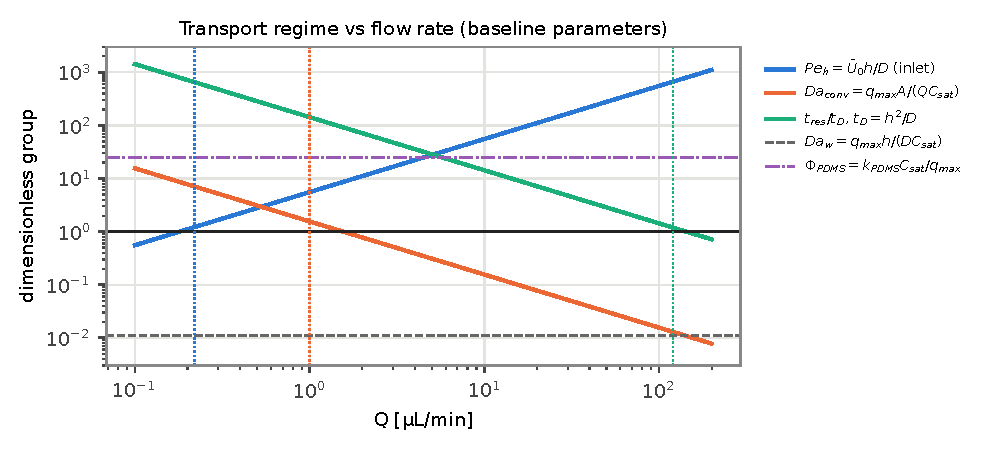
\includegraphics[width=0.9\linewidth]{oxygen_dimensionless_groups.pdf}
\caption{Oxygen transport groups against flow rate (baseline parameters) \tagM. The vertical lines mark the three simulated flow rates. Convection alone can feed the cells only where $\Da_{\mathrm{conv}}<1$, i.e.\ above \SI{1.55}{\uLmin}.}
\label{fig:o2groups}
\end{figure}

\chapter{Analytical Development of the Oxygen Transport Model}
\label{ch:o2analytical}

This chapter reduces \cref{eq:ox_cd} to a form that can be solved in closed form, in four steps.
\begin{enumerate}
\item \Cref{sec:ox_scaling} shows by scaling that the concentration is nearly uniform across the gap.
\item \Cref{sec:ox_cup} reduces the problem to an ordinary differential equation for the cup-mixing concentration.
\item \Cref{sec:ox_local} derives the exact relation between the cup-mixing concentration and the concentrations on the floor and the lid.
\item \Cref{sec:ox_imp,sec:ox_mm,sec:ox_pdms} solve the resulting equations for the impermeable, near-anoxic and PDMS/saturated cases.
\end{enumerate}
\Cref{sec:ox_numerical} describes the reduced-order (``1.5-D'') model that solves the same equations without the zero-order simplification, and \cref{sec:ox_choice} states which approximation is suitable where.

\section{Scaling: convection along, diffusion across}
\label{sec:ox_scaling}

Write \cref{eq:ox_cd} in the coordinates of the thin channel, with $x\sim\ell$ (the length over which the width changes), $y\sim w$, $z\sim h$, $u_x\sim\bar U$:
\begin{equation}
\underbrace{u_x\frac{\partial C}{\partial x}}_{\bar U\Delta C/\ell}
=D\Big(\underbrace{\frac{\partial^2C}{\partial x^2}}_{\Delta C/\ell^2}
+\underbrace{\frac{\partial^2C}{\partial y^2}}_{\Delta C/w^2}
+\underbrace{\frac{\partial^2C}{\partial z^2}}_{\Delta C/h^2}\Big).
\label{eq:ox_scaling}
\end{equation}
Relative to diffusion across the gap, axial diffusion is of order $(h/\ell)^2\le10^{-4}$ and transverse diffusion across the width is of order $(h/w)^2\le0.02$, so both are negligible. Convection relative to diffusion across the gap is of order $\Pe_h\,h/\ell$, which near the inlet ($\ell\approx\SI{50}{mm}$) is 0.004 and 0.016 at 0.22 and \SI{1}{\uLmin} and about 2 at \SI{120}{\uLmin}. At the culture flow rates, therefore, the concentration profile across the gap adjusts almost instantly to the local conditions. The axial variation is slow and is controlled by the overall balance between supply and uptake. At \SI{120}{\uLmin} the profile across the gap is still developing over the first few millimetres (\cref{sec:ox_choice}), but there the uptake changes the concentration by only about \SI{1}{\percent}.

\section{Cup-mixing balance and the role of the geometry}
\label{sec:ox_cup}

Define the flow-weighted (cup-mixing) concentration of a cross-section $S(x)$:
\begin{equation}
\Cb(x)=\frac{1}{Q}\iint_{S(x)}u_x\,C\,\dd y\,\dd z .
\end{equation}
Integrate \cref{eq:ox_cd} over the slice between $x$ and $x+\dd x$. Neglect axial diffusion, and let oxygen leave through the floor at the rate $q$ and enter through the lid at the rate $N$ per unit area, with the side walls neglected. Since $Q$ is the same in every section, this gives
\begin{equation}
Q\frac{\dd\Cb}{\dd x}=w(x)\,\big[N(x)-q(x)\big].
\label{eq:ox_cup}
\end{equation}
The geometry enters only through the width multiplying the wall fluxes. Introduce the floor area upstream of $x$,
\begin{equation}
A(x)=\int_0^xw(x')\,\dd x'=w_1L\ln\frac{L}{L-x},
\qquad\frac{\dd A}{\dd x}=w(x),
\label{eq:ox_area}
\end{equation}
so that \cref{eq:ox_cup} becomes
\begin{equation}
Q\frac{\dd\Cb}{\dd A}=N-q .
\label{eq:ox_cupA}
\end{equation}
\Cref{eq:ox_cupA} contains no geometry: per unit area of cell-covered floor, every channel shape behaves the same. The shape matters only through how fast the area accumulates along $x$. In the hyperbolic channel $A(x)$ grows faster than linearly. At $x=\SI{40}{mm}$ the floor upstream is $A=w_1L\ln5=\SI{80.5}{mm^2}$, twice that of a straight channel of width $w_1$. The widening therefore exposes the downstream cells to medium that has already passed over a large upstream area. This is the reason why low shear and low oxygen coincide in this geometry.

\section{Local profile across the gap: exact fully developed solution}
\label{sec:ox_local}

To close \cref{eq:ox_cupA} we need $q$ and $N$, which depend on the wall concentrations $\Cbot$ and $\Ctop$, not on $\Cb$. These are related by the local profile across the gap. In the quasi-equilibrium of \cref{sec:ox_scaling}, $\partial C/\partial x$ is independent of $z$ and equal to $\dd\Cb/\dd x$ (``fully developed'' mass transfer). The leading-order balance in the core of the section is then
\begin{equation}
D\frac{\partial^2C}{\partial z^2}=u_x(z)\frac{\dd\Cb}{\dd x},
\qquad u_x=\frac{6Q}{wh}\,\eta(1-\eta),\quad\eta=\frac zh .
\end{equation}
Substituting $\dd\Cb/\dd x$ from \cref{eq:ox_cup},
\begin{equation}
\frac{\dd^2C}{\dd\eta^2}=\frac{6h}{D}\,(N-q)\,\eta(1-\eta),
\qquad
\left.\frac{\dd C}{\dd\eta}\right|_{\eta=0}=\frac{qh}{D},\quad
\left.\frac{\dd C}{\dd\eta}\right|_{\eta=1}=\frac{Nh}{D},
\label{eq:ox_local_ode}
\end{equation}
where the boundary conditions are \cref{eq:ox_bc_floor,eq:ox_bc_pdms} written for the fluxes $q$ and $N$. Integrating once,
\begin{equation}
\frac{\dd C}{\dd\eta}=\frac hD\Big[q+6(N-q)\Big(\frac{\eta^2}{2}-\frac{\eta^3}{3}\Big)\Big],
\end{equation}
which satisfies the condition at $\eta=1$ automatically, as the overall balance requires. Integrating again from the floor,
\begin{equation}
C(\eta)=\Cbot+\frac hD\Big[q\,\eta+(N-q)\Big(\eta^3-\frac{\eta^4}{2}\Big)\Big].
\label{eq:ox_profile}
\end{equation}
\paragraph{Impermeable lid ($N=0$).} \Cref{eq:ox_profile} reduces to
\begin{equation}
C(\eta)-\Cbot=\frac{qh}{D}\left(\eta-\eta^3+\frac{\eta^4}{2}\right),\qquad
\Ctop-\Cbot=\frac{qh}{2D}.
\label{eq:ox_profile_imp}
\end{equation}
\paragraph{Cup-mixing relations.} Weighting \cref{eq:ox_profile} with $u_x\propto6\eta(1-\eta)$ uses the integrals $\int_0^16\eta(1-\eta)\eta\,\dd\eta=\tfrac12$ and $\int_0^16\eta(1-\eta)(\eta^3-\eta^4/2)\,\dd\eta=\tfrac{9}{70}$. The result is
\begin{equation}
\Cb-\Cbot=\frac hD\left(a_sq-a_cN\right),\qquad
\Ctop-\Cb=\frac hD\left(a_sN-a_cq\right),\qquad
a_s=\frac{13}{35},\ a_c=-\frac{9}{70}.
\label{eq:ox_superpos}
\end{equation}
For a single wall with constant flux and the other wall impermeable, the Sherwood number based on $2h$ is $\Sh=2/a_s=70/13=5.385$. For equal fluxes at both walls it is $2/(a_s+a_c)=140/17=8.235$. These are the classical values for parallel plates \citep{ShahLondon1978}, which confirms the derivation.

\paragraph{How large is the drop across the gap?} With full uptake $q=\qmax$, the floor is lower than the lid by $\qmax h/(2D)$ (IMP) or $\qmax h/D$ (balanced supply through the lid, where the profile is linear). Relative to $\Csat$, these are $\Da_w/2=\SI{0.54}{\percent}$ and $\Da_w=\SI{1.09}{\percent}$ (\cref{fig:o2_z}). Diffusion across the gap is therefore never the bottleneck. The availability of oxygen at the cells is decided by the axial balance \cref{eq:ox_cupA}.

\begin{figure}[htbp]
\centering
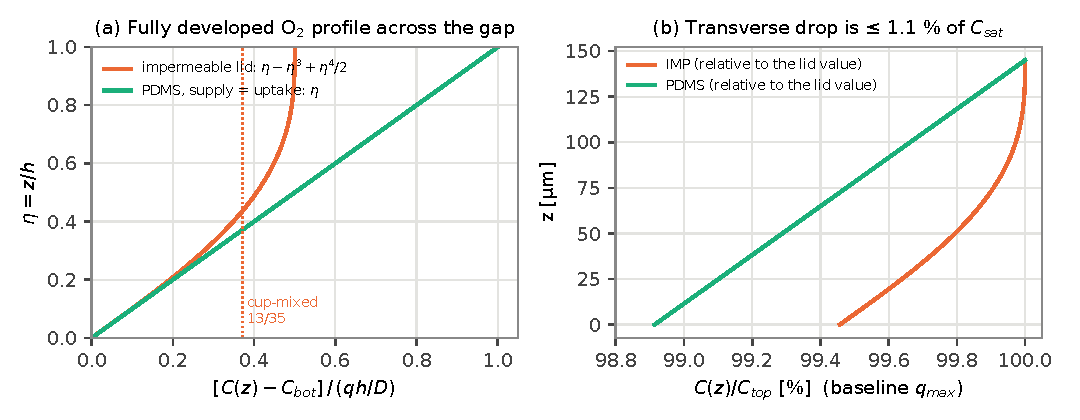
\includegraphics[width=0.95\linewidth]{oxygen_transverse_profile.pdf}
\caption{Fully developed oxygen profile across the gap \tagT. (a) Dimensionless profiles from \cref{eq:ox_profile}: impermeable lid (uptake balanced by axial depletion) and PDMS lid with supply equal to uptake (pure diffusion, linear). The dotted line is the cup-mixing value 13/35 for the impermeable lid. (b) The same profiles for the baseline uptake: the variation across the gap is at most \SI{1.1}{\percent} of the lid value.}
\label{fig:o2_z}
\end{figure}

\section{Solution I: impermeable walls, zero-order uptake}
\label{sec:ox_imp}

With $N=0$ and $q=\qmax$, \cref{eq:ox_cupA} integrates directly with $\Cb(0)=\Csat$:
\begin{equation}
\Cb(x)=\Csat-\frac{\qmax}{Q}A(x)=\Csat-\frac{\qmax w_1L}{Q}\ln\frac{L}{L-x},
\label{eq:ox_imp}
\end{equation}
and from \cref{eq:ox_superpos} the floor concentration is
\begin{equation}
\frac{\Cbot(x)}{\Csat}=1-\Da_{\mathrm{conv}}\frac{A(x)}{A_{\mathrm{cells}}}-\frac{13}{35}\Da_w .
\label{eq:ox_imp_bot}
\end{equation}
The oxygen at the cells decreases linearly with the upstream cell area, and therefore logarithmically with $x$, steepening towards the outlet. The last term is a constant offset of \SI{0.4}{\percent}. If $\Da_{\mathrm{conv}}<1$, the oxygen lost along the whole culture section is the fraction $\Da_{\mathrm{conv}}$ of the inlet supply: \SI{1.3}{\percent} at \SI{120}{\uLmin}. If $\Da_{\mathrm{conv}}>1$, the floor runs out of oxygen at the position where $\Cbot=0$. Neglecting the \SI{0.4}{\percent} offset,
\begin{equation}
x_{\mathrm{crit}}=L\left[1-\exp\!\left(-\frac{Q\Csat}{\qmax w_1L}\right)\right],
\label{eq:ox_xcrit}
\end{equation}
which is \SI{13.9}{mm} at \SI{0.22}{\uLmin} and \SI{38.7}{mm} at \SI{1}{\uLmin} \tagM. The minimum flow rate that keeps the whole culture section supplied by convection alone is
\begin{equation}
Q_{\min}=\frac{\qmax A_{\mathrm{cells}}}{\Csat}=\frac{\qmax w_1L\ln(w_{\max}/w_1)}{\Csat}=\SI{1.55}{\uLmin}.
\label{eq:ox_qmin}
\end{equation}
\Cref{eq:ox_xcrit} contains neither $D$ nor $h$. With impermeable walls the location of anoxia is set entirely by the ratio of convective supply to uptake, and changing the gap or the diffusivity does not move it. Since the shear scales as $\taw\propto Q/h^2$, a taller channel at the same shear requires a larger $Q\propto h^2$ and so delivers more oxygen. This is the coupling exploited in the design discussion of \cref{ch:o2results}.

\section{Solution II: approach to anoxia with Michaelis--Menten kinetics}
\label{sec:ox_mm}

Zero-order uptake stops being valid as $\Cbot\to\Km$. For $\Cbot\ll\Km$ the uptake is first order, $q\approx(\qmax/\Km)\Cbot$. Using $\Cbot=\Cb-a_s(h/D)q$ from \cref{eq:ox_superpos} (with $N=0$), the uptake can be written in terms of the cup-mixing concentration as two resistances in series:
\begin{equation}
q=k_{\mathrm{eff}}\,\Cb,\qquad
\frac{1}{k_{\mathrm{eff}}}=\underbrace{\frac{\Km}{\qmax}}_{\text{uptake}}+\underbrace{\frac{13}{35}\frac hD}_{\text{diffusion across }h}
=\SI{1.58e4}{}+\SI{1.80e4}{}\ \si{s/m}.
\end{equation}
\Cref{eq:ox_cupA} then gives an exponential decay in area beyond the point $A_c=A(x_{\mathrm{crit}})$:
\begin{equation}
\Cb(A)=\Cb(A_c)\exp\!\left[-\frac{k_{\mathrm{eff}}(A-A_c)}{Q}\right],
\qquad
\frac{Q}{k_{\mathrm{eff}}}=\SI{0.12}{mm^2}\ (0.22),\ \SI{0.56}{mm^2}\ (1\ \si{\uLmin}).
\label{eq:ox_mm_tail}
\end{equation}
At the local widths (\SI{1.4}{mm} and \SI{4.4}{mm}), these areas correspond to a decay length of only about \SI{0.1}{mm}. The transition from normoxia to anoxia is therefore sharp. Without the diffusion resistance, the Michaelis--Menten balance $Q\,\dd C/\dd A=-\qmax C/(\Km+C)$ has the implicit exact solution
\begin{equation}
(C-C_0)+\Km\ln\frac{C}{C_0}=-\frac{\qmax}{Q}(A-A_0),
\label{eq:ox_mm_implicit}
\end{equation}
which reduces to \cref{eq:ox_imp} for $C\gg\Km$ and to an exponential for $C\ll\Km$. In practice, $x_{\mathrm{crit}}$ from \cref{eq:ox_xcrit} marks the edge of an anoxic region with a sub-millimetre transition zone.

\section{Solution III: permeable (PDMS) and saturated lid}
\label{sec:ox_pdms}

With the Robin condition $N=\kp(\Csat-\Ctop)$, the lid concentration is eliminated using \cref{eq:ox_superpos}:
\begin{equation}
N=k'\left[(\Csat-\Cb)-\frac{9}{70}\frac hDq\right],\qquad
k'=\frac{\kp}{1+\frac{13}{35}\Bi}=\SI{5.13e-6}{m/s}.
\label{eq:ox_N}
\end{equation}
With zero-order uptake ($q=\qmax$, valid because $C\gg\Km$ throughout, as shown below), \cref{eq:ox_cupA} is a linear first-order equation in $\Cb$:
\begin{equation}
Q\frac{\dd\Cb}{\dd A}=k'\left(\Cb_\infty-\Cb\right),\qquad
\Cb_\infty=\Csat-\frac{\qmax}{k'}-\frac{9}{70}\frac{h\qmax}{D},
\end{equation}
with solution
\begin{equation}
\Cb(x)=\Cb_\infty+(\Csat-\Cb_\infty)\exp\!\left[-\frac{k'A(x)}{Q}\right].
\label{eq:ox_pdms}
\end{equation}
The cup-mixing concentration relaxes exponentially, in terms of the upstream cell area, to an equilibrium in which the lid supplies exactly what the cells consume. In that equilibrium $N=\qmax$, the profile across the gap is linear, and from $\Ctop=\Csat-\qmax/\kp$ and $\Ctop-\Cbot=\qmax h/D$,
\begin{equation}
\frac{C_{\mathrm{bot},\infty}}{\Csat}=1-\frac{1}{\Phi_{\mathrm{PDMS}}}-\Da_w=1-0.040-0.011=0.949 .
\label{eq:ox_pdms_inf}
\end{equation}
This depends neither on $Q$ nor on the geometry. The relaxation area $Q/k'$ converts through \cref{eq:ox_area} into a relaxation length from the inlet, $x^*=L[1-\exp(-Q/(k'w_1L))]$. It is \SI{0.71}{mm} at \SI{0.22}{\uLmin} and \SI{3.1}{mm} at \SI{1}{\uLmin}, so the equilibrium governs almost the whole channel. At \SI{120}{\uLmin}, $Q/k'=\SI{390}{mm^2}$ exceeds the whole cell area, so the lid hardly matters: convection keeps the concentration near $\Csat$.

\paragraph{Saturated lid.} For $\kp\to\infty$, $k'\to D/(a_sh)$, the equilibrium is $C_{\mathrm{bot},\infty}=\Csat(1-\Da_w)=0.989\,\Csat$, and it is reached within $x^*=0.07$, 0.30 and \SI{25.6}{mm} at the three flow rates.

\paragraph{Validity.} With the baseline parameters $\Cbot\ge0.95\,\Csat=268\,\Km$, so the zero-order assumption holds to better than \SI{0.4}{\percent}. The PDMS result requires $\Phi_{\mathrm{PDMS}}>1$. If the lid permeability or thickness were such that $\kp\Csat<\qmax$, the lid alone could not feed the cells, and the IMP-type depletion of \cref{sec:ox_imp} would reappear, delayed in $x$.

\section{Reduced-order numerical model (1.5-D)}
\label{sec:ox_numerical}

The closed forms use zero-order kinetics. The general case, with Michaelis--Menten uptake, any lid condition and any flow rate, is solved by integrating \cref{eq:ox_cup} numerically. At each $x$ the local fluxes are found from three coupled algebraic relations,
\begin{equation}
q=\qmax\frac{\Cbot}{\Km+\Cbot},\qquad
\Cbot=\Cb-\frac hD\left(a_sq-a_cN\right),\qquad
N=k'\left[(\Csat-\Cb)+a_c\frac hDq\right],
\end{equation}
which reduce to one non-linear equation for $q$, solved by bisection (Brent's method). The ODE is integrated with an adaptive Runge--Kutta method (relative tolerance $10^{-8}$) from $\Cb(0)=\Csat$ to $x_t$ (code in \cref{app:repro}). Two checks were made:
\begin{itemize}
\item the integrated uptake equals the oxygen lost by the flow to within \SI{0.03}{\percent} in all nine cases (global mass balance);
\item in the zero-order range the numerical solution reproduces the closed forms \cref{eq:ox_imp,eq:ox_pdms} (\cref{fig:o2_axial}); for example, at $x=\SI{45}{mm}$ and \SI{1}{\uLmin} with a PDMS lid, $\Cbot/\Csat=0.9496$ (numerical) against 0.9494 (closed form).
\end{itemize}

\section{Which approximation is suitable where}
\label{sec:ox_choice}

\begin{table}[htbp]
\centering
\caption{Analytical approximations for oxygen transport in the widening chip and their range of validity.}
\label{tab:ox_models}
\small
\begin{tabularx}{\linewidth}{@{}p{0.27\linewidth}X p{0.2\linewidth}@{}}
\toprule
Approximation & Valid when & Use\\
\midrule
Pure diffusion across the gap (linear profile) & local supply equals uptake ($\dd\Cb/\dd x=0$) & PDMS/SAT equilibrium\\
Fully developed profile, \cref{eq:ox_superpos} & $\Pe_h h/\ell\ll1$; beyond the concentration entrance length & 0.22 and \SI{1}{\uLmin}; all $x$\\
Cup-mixing balance \cref{eq:ox_cupA} & $\Pe_L\gg1$; side walls negligible & all cases\\
Zero-order closed forms (I, III) & $\Cbot\gg\Km$ & before $x_{\mathrm{crit}}$; PDMS/SAT everywhere\\
First-order tail (II) & $\Cbot\ll\Km$ & just beyond $x_{\mathrm{crit}}$\\
Full MM, 1.5-D numerical & all of the above but kinetics general & reference solution\\
3D CFD (UDS) & always & side-wall layers, outlet corner\\
\bottomrule
\end{tabularx}
\end{table}

The concentration entrance length for parallel plates, $L_c\approx0.0115\,\Pe_{2h}\,(2h)$ \citep{ShahLondon1978} with $\Pe_{2h}=\bar U_0\,2h/D$, is 0.008, 0.037 and \SI{4.4}{mm} at the three flow rates. Within it, the concentration boundary layer on the floor is thinner than the gap and $\Cbot$ is closer to $\Cb$ than the fully developed relation predicts. The fully developed model therefore slightly over-predicts the depletion near the inlet at \SI{120}{\uLmin}, by at most $a_s\Da_w=\SI{0.4}{\percent}$ of $\Csat$. This error is conservative and negligible. A Lévêque-type developing-layer analysis is therefore unnecessary. The most suitable model for this geometry is the cup-mixing balance with the exact fully developed closure. It is accurate wherever the lubrication flow is accurate, and it misses only the three-dimensional side-wall and corner effects.

\chapter{Oxygen Transport Results and Discussion}
\label{ch:o2results}

\begin{keybox}[Status of the results in this chapter]
All results here are \textbf{model predictions} \tagM\ from the closed forms of \cref{ch:o2analytical} and the 1.5-D model. They use the validated lubrication flow, but the uptake parameters are illustrative (\cref{tab:o2params}). No oxygen CFD or measurement was available. The ``analytical against numerical'' comparison is between the closed forms and the numerically integrated reduced-order model, not against Fluent.
\end{keybox}

\section{Axial distribution of oxygen at the cell layer}

\Cref{fig:o2_axial} shows the oxygen concentration on the floor along the axis for the three flow rates and the three lid conditions. \Cref{tab:o2_results} gives the station values and summary metrics. The imaging window is $5\le x\le\SI{40}{mm}$.

\begin{figure}[htbp]
\centering
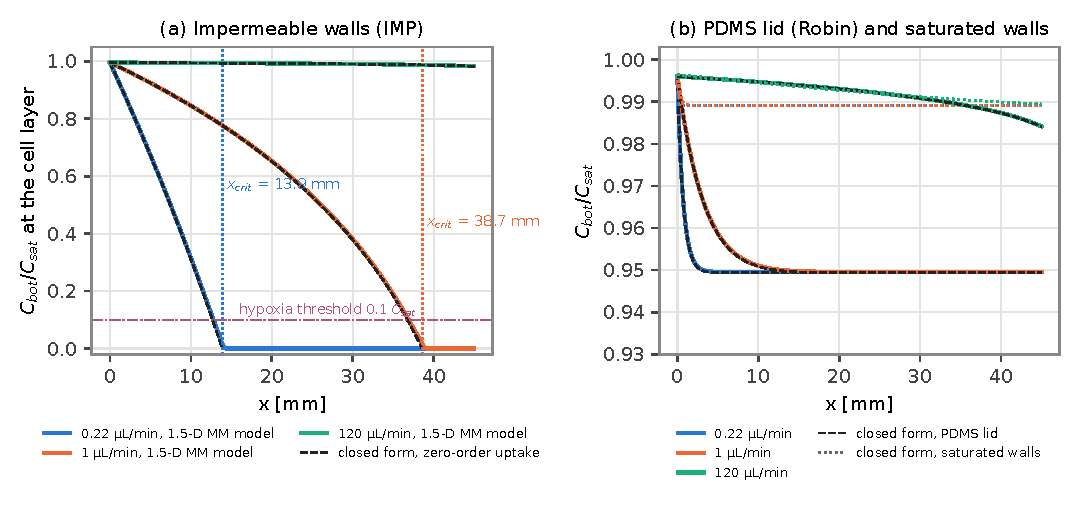
\includegraphics[width=\linewidth]{oxygen_axial_profiles.pdf}
\caption{Oxygen at the cell layer along the channel, $\Cbot/\Csat$ \tagM. Coloured lines: 1.5-D model with Michaelis--Menten uptake. Black dashed lines: closed forms with zero-order uptake, \cref{eq:ox_imp_bot} and \cref{eq:ox_pdms}. Dotted lines in (b): closed form for a saturated lid. (a) With impermeable walls the floor becomes anoxic beyond $x_{\mathrm{crit}}=13.9$ and \SI{38.7}{mm} at 0.22 and \SI{1}{\uLmin}. (b) With a \SI{5}{mm} PDMS lid the concentration relaxes within 1--\SI{3}{mm} to the lid equilibrium $0.949\,\Csat$, independent of $Q$. At \SI{120}{\uLmin} convection dominates and all three walls give 0.98--\SI{1.00}{}$\,\Csat$.}
\label{fig:o2_axial}
\end{figure}

\begin{table}[htbp]
\centering
\caption{Oxygen at the cell layer, $\Cbot/\Csat$, from the 1.5-D model with baseline parameters \tagM. Window = $5\le x\le\SI{40}{mm}$; ``hypoxic'' = area fraction of the window with $\Cbot<0.1\,\Csat$.}
\label{tab:o2_results}
\small
\resizebox{\linewidth}{!}{%
\begin{tabular}{@{}llccccccccc@{}}
\toprule
$Q$ & Lid & S1 & S2 & S3 & S4 & S5 & Mean in & Min in & Hypoxic & $\Cb_{\mathrm{out}}/\Csat$\\
{[}\ulmin{]} & & & & & & & window & window & fraction & ($x=\SI{45}{mm}$)\\
\midrule
0.22 & IMP  & 0.675 & 0.000 & 0.000 & 0.000 & 0.000 & 0.050 & 0.000 & 0.87 & 0.000\\
0.22 & PDMS & 0.950 & 0.950 & 0.950 & 0.950 & 0.950 & 0.950 & 0.950 & 0 & 0.955\\
0.22 & SAT  & 0.989 & 0.989 & 0.989 & 0.989 & 0.989 & 0.989 & 0.989 & 0 & 0.995\\
\addlinespace
1 & IMP  & 0.925 & 0.757 & 0.531 & 0.190 & 0.000 & 0.426 & 0.000 & 0.18 & 0.000\\
1 & PDMS & 0.959 & 0.950 & 0.950 & 0.950 & 0.950 & 0.950 & 0.950 & 0 & 0.955\\
1 & SAT  & 0.989 & 0.989 & 0.989 & 0.989 & 0.989 & 0.989 & 0.989 & 0 & 0.995\\
\addlinespace
120 & IMP  & 0.995 & 0.994 & 0.992 & 0.989 & 0.983 & 0.991 & 0.987 & 0 & 0.987\\
120 & PDMS & 0.995 & 0.994 & 0.992 & 0.989 & 0.984 & 0.991 & 0.987 & 0 & 0.988\\
120 & SAT  & 0.995 & 0.994 & 0.992 & 0.991 & 0.989 & 0.992 & 0.990 & 0 & 0.995\\
\bottomrule
\end{tabular}}
\end{table}

\section{Discussion of the guiding questions}

\paragraph{1. How does the oxygen concentration vary in space?} Along the channel, the concentration is governed by \cref{eq:ox_cupA}: it falls in proportion to the cell area already passed, unless the lid replaces what is consumed. Across the gap it varies by at most \SI{1.1}{\percent} (\cref{fig:o2_z}), because diffusion across \SI{145}{\micro\metre} takes \SI{7}{s} while the medium spends 17--\SI{76}{min} in the culture section at the two culture flow rates. Across the width, the reduced-order model assumes no variation. The CFD flow field, however, shows a \SI{0.13}{mm} side-wall layer of slower fluid (\cref{sec:val_transverse}), where the residence time is longer and the depletion with impermeable walls will be stronger.

\paragraph{2. Where are the highest and lowest concentrations?} The highest concentrations are at the inlet, $\Csat$ by definition. With impermeable walls the lowest are downstream: the floor is anoxic beyond \SI{13.9}{mm} at \SI{0.22}{\uLmin} (\SI{87}{\percent} of the imaging window hypoxic) and beyond \SI{38.7}{mm} at \SI{1}{\uLmin} (\SI{18}{\percent} hypoxic, in the S4--S5 region). With a PDMS lid, the minimum, $0.949\,\Csat$, is reached a few millimetres from the inlet and then stays constant.

\paragraph{3. Relative importance of convection and diffusion.} Diffusion controls transport across the gap and convection controls transport along the channel ($\Pe_L\ge421$, $t_D/t_{\mathrm{res}}\le\num{7e-3}$ at the culture flow rates). The competition that matters is between convective \emph{supply} and \emph{uptake}, measured by $\Da_{\mathrm{conv}}$: 7.06, 1.55 and 0.013. The ``P\'eclet number'' in the usual sense does not decide oxygen availability here. $\Pe_h$ is 1.2 at \SI{0.22}{\uLmin}, and yet the floor is anoxic over most of the channel.

\paragraph{4. How does the velocity field influence oxygen transport?} Only through the flow rate (the convective capacity $Q\Csat$) and the shape of the profile across the gap (the factors 13/35 and 9/70 in \cref{eq:ox_superpos}). Because the flow is a Stokes flow, the oxygen field at a given $Q$ is independent of the absolute velocity magnitude. The \SI{-5}{\percent} CFD offset therefore has no bearing on these results.

\paragraph{5. Does the geometry help or hinder oxygen delivery?} It hinders it in the low-shear region. In a straight channel of width $w_1$, the cell area upstream of $x=\SI{40}{mm}$ would be \SI{40}{mm^2}; in the hyperbolic channel it is \SI{80.5}{mm^2}. Per unit flow, the downstream cells receive medium that has fed twice as many cells. The geometry that creates a linear shear gradient also creates a steepening oxygen gradient in the same direction (\cref{eq:ox_imp_bot}).

\paragraph{6. How does oxygen change along the flow direction?} With impermeable walls, it falls in proportion to $\ln[L/(L-x)]$, slowly at first and then faster, until anoxia at $x_{\mathrm{crit}}$. Beyond that point there is a sharp transition (decay length about \SI{0.1}{mm}, \cref{sec:ox_mm}). With a PDMS lid, the concentration falls exponentially in $A(x)$ to a plateau. At \SI{120}{\uLmin} it falls almost linearly by 1--\SI{2}{\percent}.

\paragraph{7. Role of the wall boundary condition.} The lid condition is decisive at the culture flow rates (\cref{fig:o2_axial}). With an impermeable lid, oxygen availability is set by the flow and is poor. With a \SI{5}{mm} PDMS lid it is set by the lid and is good at every flow rate, because the lid can supply 25 times the maximum uptake ($\Phi_{\mathrm{PDMS}}=25.1$). With a PDMS lid at 0.22 and \SI{1}{\uLmin}, about \SIrange{97}{99}{\percent} of the oxygen consumed is supplied through the lid and only 1--\SI{3}{\percent} by the flow. At \SI{120}{\uLmin} the lid supplies only about \SI{11}{\percent}. Whether cells in this device are hypoxic is therefore decided by the PDMS, not by the flow, provided the lid is exposed to incubator air and has its nominal permeability.

\paragraph{8. Influence of the consumption model.} With Michaelis--Menten kinetics and $\Csat/\Km=283$, the uptake is effectively zero order wherever $\Cbot>0.03\,\Csat$. The closed forms with zero-order uptake coincide with the numerical model up to $x_{\mathrm{crit}}$ (\cref{fig:o2_axial}a), and the choice of $\Km$ only affects the sub-millimetre transition zone. A first-order model, $q=(\qmax/\Km)C$, would be wrong by a factor of up to 280 at normoxic concentrations. The parameters that control the results are $\qmax$ (cell density $\times$ uptake per cell) and $\kp$, not $\Km$.

\paragraph{9. Effect of the flow rate.} With impermeable walls, increasing $Q$ moves $x_{\mathrm{crit}}$ downstream, in proportion to $1-\exp(-Q\Csat/\qmax w_1L)$, and removes anoxia altogether above $Q_{\min}=\SI{1.55}{\uLmin}$. At \SI{120}{\uLmin} the depletion is \SI{1.3}{\percent}. With a PDMS lid the flow rate barely matters at 0.22 and \SI{1}{\uLmin} (equilibrium $0.949\,\Csat$), and at \SI{120}{\uLmin} convection keeps the concentration even higher (0.983--$0.995\,\Csat$).

\section{Shear and oxygen together}

\Cref{fig:o2_tau} plots the oxygen at the cell layer against the local wall shear over the imaging window. With impermeable walls, the cells exposed to the lowest shear are also the cells starved of oxygen. At \SI{0.22}{\uLmin} every cell below about \SI{0.008}{\dyncm} is anoxic, and at \SI{1}{\uLmin} every cell below about \SI{0.010}{\dyncm}. A shear-response experiment in an impermeable device would therefore confound shear and hypoxia in exactly the part of the shear range that the device was designed to explore. With a PDMS lid the oxygen is uniform ($0.95\,\Csat$) across the whole shear range, so shear is the only variable.

\begin{figure}[htbp]
\centering
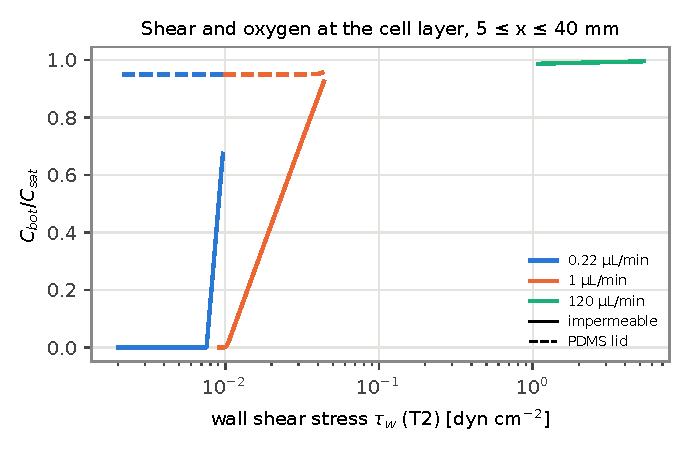
\includegraphics[width=0.62\linewidth]{oxygen_vs_shear.pdf}
\caption{Oxygen at the cell layer against wall shear (T2) for $5\le x\le\SI{40}{mm}$ \tagM. Solid: impermeable walls. Dashed: \SI{5}{mm} PDMS lid. With impermeable walls the lowest shear coincides with anoxia at 0.22 and \SI{1}{\uLmin}.}
\label{fig:o2_tau}
\end{figure}

\section{Quantitative interpretation}

\begin{table}[htbp]
\centering
\caption{Oxygen budget of the culture section \tagM. Rates in \si{mol/s}; ``demand met'' is the actual uptake divided by the maximum uptake $\qmax A_{\mathrm{cells}}$.}
\label{tab:o2_budget}
\small
\begin{tabular}{@{}lccc@{}}
\toprule
Quantity & \SI{0.22}{\uLmin} & \SI{1}{\uLmin} & \SI{120}{\uLmin}\\
\midrule
Convective supply $Q\Csat$ & \num{6.53e-13} & \num{2.97e-12} & \num{3.56e-10}\\
Maximum uptake $\qmax A_{\mathrm{cells}}$ & \num{4.61e-12} & \num{4.61e-12} & \num{4.61e-12}\\
Maximum lid supply $\kp\Csat A_{\mathrm{cells}}$ & \num{1.16e-10} & \num{1.16e-10} & \num{1.16e-10}\\
Actual uptake, IMP & \num{6.53e-13} & \num{2.97e-12} & \num{4.59e-12}\\
Demand met, IMP & \SI{14}{\percent} & \SI{64}{\percent} & \SI{99.6}{\percent}\\
Actual uptake, PDMS & \num{4.59e-12} & \num{4.59e-12} & \num{4.59e-12}\\
Depletion at $x=\SI{45}{mm}$, IMP ($1-\Cb/\Csat$) & \SI{100}{\percent} & \SI{100}{\percent} & \SI{1.3}{\percent}\\
Depletion at $x=\SI{45}{mm}$, PDMS & \SI{4.5}{\percent} & \SI{4.5}{\percent} & \SI{1.2}{\percent}\\
Diffusion time across gap $t_D$ [s] & 7.0 & 7.0 & 7.0\\
Residence time $t_{\mathrm{res}}$ [s] & 4553 & 1002 & 8.3\\
Onset of anoxia, IMP [mm] & 13.9 & 38.7 & none\\
PDMS relaxation length $x^*$ [mm] & 0.71 & 3.1 & $>45$\\
\bottomrule
\end{tabular}
\end{table}

\Cref{tab:o2_budget} gives the budget. With impermeable walls at \SI{0.22}{\uLmin} the flow delivers only \SI{14}{\percent} of what the cells could consume, and at \SI{1}{\uLmin} \SI{64}{\percent}. In both cases the outlet medium is fully depleted. The flux of oxygen into the cell layer is $\qmax=\SI{4e-8}{mol.m^{-2}.s^{-1}}$ wherever $\Cbot\gg\Km$ and falls to zero in the anoxic zone. With a PDMS lid the full demand is met at every flow rate.

\paragraph{Sensitivity.} \Cref{tab:o2_sens} and \cref{fig:o2_design} show how the conclusions depend on the uncertain parameters. Using the closed forms, the effects can be read off directly:
\begin{itemize}
\item $\qmax$ dominates. The plausible range of \num{0.5e-8} to \SI{50e-8}{mol.m^{-2}.s^{-1}} changes $Q_{\min}$ from 0.19 to \SI{19}{\uLmin}.
\item With a PDMS lid the floor stays above $0.87\,\Csat$ up to $\qmax=\SI{1e-7}{mol.m^{-2}.s^{-1}}$. Only at the extreme value of \num{5e-7} would it fall to $0.37\,\Csat$.
\item $\Csat$, $D$ and the lid properties change the results by a few percent.
\end{itemize}
The two quantities that must be measured before any oxygen conclusion is drawn for Caco-2 or A549 cells are therefore the oxygen consumption per cell and the cell density at confluence.

\begin{table}[htbp]
\centering
\caption{Sensitivity of the closed-form predictions \tagM. Bold = baseline. $C_{\mathrm{bot},\infty}$ is the PDMS-lid equilibrium, \cref{eq:ox_pdms_inf}.}
\label{tab:o2_sens}
\small
\resizebox{\linewidth}{!}{%
\begin{tabular}{@{}lccccc@{}}
\toprule
Case & $Q_{\min}$ [\ulmin] & $x_{\mathrm{crit}}$ at 0.22 [mm] & $x_{\mathrm{crit}}$ at 1 [mm] & $\Phi_{\mathrm{PDMS}}$ & $C_{\mathrm{bot},\infty}/\Csat$ (PDMS)\\
\midrule
\textbf{Baseline} & \textbf{1.55} & \textbf{13.9} & \textbf{38.7} & \textbf{25.1} & \textbf{0.949}\\
$\qmax=\num{0.5e-8}$ & 0.19 & none & none & 201 & 0.994\\
$\qmax=\num{10e-8}$ & 3.88 & 6.1 & 22.4 & 10.1 & 0.873\\
$\qmax=\num{50e-8}$ & 19.4 & 1.3 & 5.6 & 2.0 & 0.367\\
$\Csat=0.167$ / 0.200 & 1.65 / 1.38 & 13.2 / 15.3 & 37.6 / 40.6 & 23.6 / 28.2 & 0.946 / 0.955\\
$D=\SI{2.6e-9}{m^2/s}$ & 1.55 & 13.9 & 38.7 & 25.1 & 0.948\\
PDMS 600 Barrer & 1.55 & 13.9 & 38.7 & 18.9 & 0.936\\
PDMS 8 mm / 3 mm thick & 1.55 & 13.9 & 38.7 & 15.7 / 41.9 & 0.926 / 0.965\\
\bottomrule
\end{tabular}}
\end{table}

\begin{figure}[htbp]
\centering
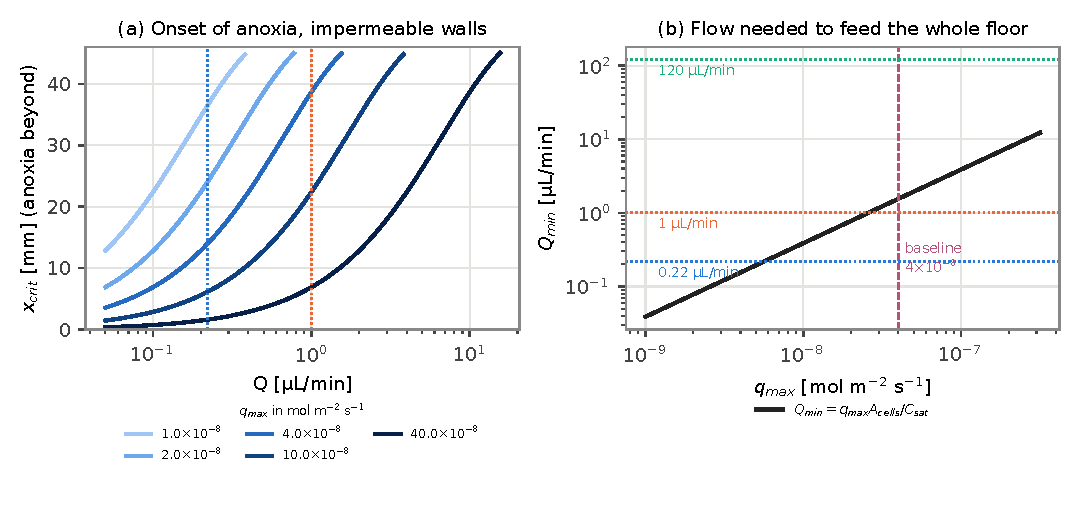
\includegraphics[width=\linewidth]{oxygen_design_map.pdf}
\caption{Design maps from the closed forms (impermeable walls) \tagM. (a) Position beyond which the floor is anoxic, \cref{eq:ox_xcrit}, against flow rate for a range of $\qmax$. Dotted lines: 0.22 and \SI{1}{\uLmin}. (b) Minimum flow rate that feeds the whole culture section by convection alone, \cref{eq:ox_qmin}.}
\label{fig:o2_design}
\end{figure}

\section{Engineering implications}

\begin{enumerate}
\item \textbf{Low shear and low oxygen coincide in this geometry.} The device delivers its lowest shear exactly where its oxygen supply by convection is lowest. In a device with impermeable walls (glass, thermoplastics, or PDMS whose surface is sealed or coated) a shear experiment at \SI{\le1}{\uLmin} would expose the downstream cells to hypoxia. This would be invisible in a flow simulation.
\item \textbf{A PDMS lid keeps the cells oxygenated in the model.} With a \SI{5}{mm} PDMS lid exposed to incubator air, the model predicts $\Cbot\ge0.95\,\Csat$ everywhere, at any flow rate. The device as published is therefore probably well oxygenated, but this depends on the lid being permeable in practice. Measurements in perfused PDMS reactors have shown axial oxygen gradients despite PDMS walls \citep{Mehta2007}. Immersing the device in water, as suggested in the protocol to limit bubbles \citep{Delon2020}, would add a transport resistance. These effects should be quantified (with oxygen-sensing films or probes) before the device is used for long-term studies at low flow.
\item \textbf{Operational levers.} With an impermeable device, run at $Q>Q_{\min}=\qmax A_{\mathrm{cells}}/\Csat$. With the baseline uptake this is \SI{1.55}{\uLmin}, which raises the shear accordingly. Alternatively, oxygenate the medium above air saturation (raising $\Csat$), or seed at lower density (lowering $\qmax$).
\item \textbf{Geometric levers.} The shear scales as $\taw\propto Q/(h^2w)$ and the oxygen supply as $Q$. To reach a target shear with more oxygen, increase the height: at constant shear $Q\propto h^2$. Doubling $h$ from 145 to \SI{290}{\micro\metre} would allow four times the flow at the same shear and would cut $\Da_{\mathrm{conv}}$ by four. The cost is thicker side-wall layers ($\delta\propto h$) and a weaker Hele-Shaw approximation ($h/w$ doubles). Reducing $w_{\max}/w_1$ or $L$ reduces the cell area, and hence the uptake, but also the shear range. A thinner PDMS lid increases $\Phi_{\mathrm{PDMS}}$ in proportion to $1/t_{\mathrm{PDMS}}$.
\end{enumerate}

\begin{keybox}[Answer to RQ4--RQ5]
The widening geometry accumulates cell area faster than length, so the cells in the low-shear, downstream region receive the most depleted medium. With impermeable walls and illustrative uptake, convection cannot feed the cells below $Q_{\min}=\SI{1.55}{\uLmin}$: anoxia is predicted beyond \SI{13.9}{mm} (\SI{0.22}{\uLmin}) and \SI{38.7}{mm} (\SI{1}{\uLmin}), coinciding with the lowest shear. A \SI{5}{mm} PDMS lid can supply 25 times the uptake and would hold the cell layer at $0.95\,\Csat$ at every flow rate. Oxygen availability in this device is therefore decided by the walls and the cell uptake, not by the flow. The key unknowns are the measured uptake rate and the effective permeability of the lid.
\end{keybox}

\chapter{Integrated Discussion}
\label{ch:discussion}

\section{From geometry to oxygen: how the parts connect}

The project followed one chain of reasoning. The hyperbolic width was chosen so that $1/w(x)$ is linear in $x$. Lubrication theory turns this into a linear pressure gradient and a linear wall shear (\cref{ch:theory}). The CFD confirmed that this design principle holds where the theory's assumptions hold. It also showed precisely where they do not: near the narrow inlet (side-wall drag) and at the outlet corner (two-dimensional flow). Having established that the flow is a Stokes flow whose shape is known to within \SI{1}{\percent}, we could use the same lubrication flow as the transport field for oxygen. The oxygen analysis then showed that the defining feature of the design, the widening that spreads a fixed flow over a growing area, controls the oxygen supply as strongly as it controls the shear.

\section{What was reproduced}

\begin{itemize}
\item The shear range of the reference paper at both flow rates (within a few percent at the inlet), the raised shear minimum near the outlet, and the imaging zones at S3--S4 (within \SI{2}{\percent}).
\item The linear decrease of shear along the axis, accurate to about $\pm\SI{4}{\percent}$ for $x\lesssim\SI{40}{mm}$.
\item The independence of the uniform-shear zone from the flow rate. In the present results this follows from exact Stokes scaling (\SI{0.08}{\percent} over a 545-fold range of $Q$).
\end{itemize}
Not reproduced, or not reproducible from the information available: the published $D_{\max}$ at S5, the published mesh sensitivity of \SI{1.4}{\percent}, and the velocity and strain-rate profiles across the gap.

\section{How accurate is the theory?}

Eq.~2 of the reference paper is a good design formula over most of the channel, but for a reason the paper does not discuss. Its error is systematic. It under-predicts the shear by up to \SI{10}{\percent} near the inlet, because it neglects side-wall drag, and it fails completely at S5, because the outlet corner makes the flow two-dimensional. The present CFD reproduces both effects exactly in shape, but carries a \SI{-5}{\percent} offset, so its \emph{apparent} agreement with Eq.~2 ($\pm\SI{3.3}{\percent}$ at S1--S4) is partly a cancellation. This illustrates a general caution: a close match between CFD and a simple formula is not by itself evidence that either is correct. The structure of the residual had to be examined against a hierarchy of theories (T1--T3) to find this out.

T2 and T3 together explain every systematic feature of the CFD, apart from the uniform offset: the slope of the deviation with $h/w$, the position of the shear minimum, the \SI{46}{\percent} excess at S5, the side-wall layer and the dome-shaped profile at S5.

\section{Physical phenomena identified}

\begin{enumerate}
\item \textbf{Stokes linearity.} All fields are proportional to $Q$; inertia appears only as a \SI{0.7}{\percent} effect at the inlet face at \SI{120}{\uLmin}.
\item \textbf{Side-wall drag.} The side walls raise the axial shear by $\approx0.63\,h/w$ and create a non-uniform layer about $0.9h$ thick that does not change along the channel. This is why the uniform fraction of the width grows downstream.
\item \textbf{Two-dimensional redistribution at the outlet corner.} Within about \SI{3}{mm} of $x_t$ the flow turns towards the outlet. The shear on the axis rises by \SI{46}{\percent} relative to Eq.~2 and the corners stagnate.
\item \textbf{Numerical under-resolution across the gap.} The peak velocity exceeds the parabola implied by the computed pressure gradient. This is a measurable signature of too few cells across the gap, which can be tested.
\end{enumerate}

\section{What oxygen modelling adds}

The flow analysis answers the question ``what shear do the cells feel?'' The oxygen analysis answers ``is shear the only thing that differs between the cells?'' For an impermeable device at the culture flow rates, the answer is no. The low-shear region is also the oxygen-starved region, so a biological gradient along the channel could not be attributed to shear alone. For the actual PDMS device, the model indicates that oxygen is uniform at about \SI{95}{\percent} of saturation. If confirmed, this validates the device for shear studies in a way the flow analysis alone could not. Three further results came only from the transport analysis:
\begin{itemize}
\item the controlling group $\Da_{\mathrm{conv}}$ and the threshold $Q_{\min}=\qmax A_{\mathrm{cells}}/\Csat$;
\item the independence of the anoxia position from $h$ and $D$ with impermeable walls;
\item the $Q$-independent PDMS equilibrium $1-1/\Phi_{\mathrm{PDMS}}-\Da_w$.
\end{itemize}

\section{Limitations of the current approach}

The flow validation rests on one mesh and on exports that lack the gap coordinate. The oxygen analysis rests on illustrative uptake parameters and on a reduced-order model that cannot resolve the side-wall layers or the corner. Both limitations are discussed in \cref{ch:limitations}, and the information missing for each is listed in \cref{app:missing}.

\chapter{Limitations, Scope for Improvement and Future Work}
\label{ch:limitations}

\section{Limitations}

\paragraph{Theoretical assumptions.}
\begin{itemize}
\item T1 assumes infinite plates and a slowly varying planform. It is invalid near S5 and in the outlet.
\item T2 assumes locally fully developed flow in each rectangular section.
\item T3 is depth-averaged and does not resolve the side-wall layer or three-dimensional effects at the corners.
\item All three are Stokes-flow models. This is justified by the CFD, which shows a non-linearity of at most \SI{0.7}{\percent}.
\end{itemize}

\paragraph{Idealised boundary conditions.} The inflow enters as a uniform velocity at the face of a \SI{2}{mm} lead-in. The punched ports, tubing and bubble trap of the real device were not modelled. The outlet is at a fixed pressure. These choices do not affect the hyperbolic section, but they do affect the absolute pressures.

\paragraph{Numerical discretisation and mesh resolution.} Only one mesh was run. About nine cells span the gap and the wall nodes are \SIrange{0.08}{0.10}{mm} apart near the side walls. The uniform \SI{-5}{\percent} offset of shear and pressure gradient is most probably discretisation error, but this has not been demonstrated. The mesh type and quality metrics were not documented in the exports.

\paragraph{Missing data and convergence evidence.} The channel height and the lead-in were inferred rather than read from the set-up. The velocity was exported without the $z$ coordinate. Neither the residual history nor the mass balance was exported.

\paragraph{Reference data.} The published results are available only as plots and ranges. The paper's height, length and uniformity criterion are partly inconsistent, so the comparison with it is semi-quantitative.

\paragraph{Oxygen model.}
\begin{itemize}
\item The uptake parameters ($\qmax$, $\Km$) are illustrative, not measured for Caco-2 or A549 cells, and the conclusions depend on $\qmax$ above all.
\item The model is steady. It ignores re-oxygenation transients after medium changes and the hours needed to equilibrate the PDMS.
\item The PDMS is represented by a steady Robin coefficient. Partitioning, diffusion inside the PDMS, water immersion and permeability loss by protein adsorption are not modelled.
\item The reduced-order model is uniform across the width. It neglects the slower side-wall layers, where depletion with impermeable walls will be stronger.
\item The monolayer is a surface flux. Cell height, its effect on the flow and the variation of uptake with shear or with cell differentiation are ignored.
\item There is no experimental validation of any oxygen prediction.
\end{itemize}

\section{Future work}

Each item below addresses one of the limitations above.

\begin{enumerate}
\item \textbf{Mesh-independence study (highest priority).} Run the two-factor study of \cref{sec:num_gci} at \SI{1}{\uLmin} ($N_z=9$, 18, 36; $\Delta s=100$, 50, \SI{25}{\micro\metre}) and report $\mathrm{GCI}_{\mathrm{fine}}$, the observed order and the extrapolated values. If the shear rises towards T2 with $N_z$, the \SI{-5}{\percent} offset is confirmed as discretisation error and the absolute CFD values can be corrected.
\item \textbf{Complete exports.} Report the inlet/outlet mass flux, the residual history and the domain extents. Export $u_x(z)$ along lines at S1--S5, so the parabola and a profile-fit wall shear can be tested, and export the floor ($z=0$) wall shear alone along fine lines across the width.
\item \textbf{Oxygen CFD.} Run the prepared Fluent case: one user-defined scalar (UDS) on the frozen flow, with the Michaelis--Menten floor flux and the PDMS Robin flux implemented as user-defined functions (UDFs). Start with the mandatory sign and mass-balance test (zero-order uptake with impermeable walls must satisfy $Q(\Csat-\Cb_{\mathrm{out}})=\qmax A_{\mathrm{cells}}$). Then run IMP, PDMS and SAT at the three flow rates, and compare with \cref{tab:o2_results}. The CFD will quantify the extra depletion in the side-wall layers and near the outlet corner, which the reduced-order model cannot capture.
\item \textbf{Transient oxygen transport.} Simulate re-oxygenation after a medium change or a change of flow, over 1--\SI{2}{h}.
\item \textbf{Conjugate PDMS transport.} Model oxygen transport inside the lid and side walls (solved in partial pressure, to handle partitioning). Vary the lid thickness, permeability ageing and water immersion.
\item \textbf{Measured kinetics.} Measure the oxygen consumption rate and the confluent density of the cell lines, and replace the illustrative $\qmax$ and $\Km$. Consider uptake that depends on the shear or on the differentiation state of the cells.
\item \textbf{Experimental validation.} Measure the pressure drop (flow), and the oxygen concentration at the floor using an oxygen-sensing film (for example a PtTFPP optode) along the channel at 0.22 and \SI{1}{\uLmin}.
\item \textbf{Parametric design.} Use the closed forms to choose $h$, $w_1$, $L$ and $Q$ that meet a target shear range while keeping $\Da_{\mathrm{conv}}<1$ or $\Phi_{\mathrm{PDMS}}\gg1$. Check selected designs with CFD.
\end{enumerate}

\chapter{Conclusion}
\label{ch:conclusion}

This project set out to reproduce the widening Hele-Shaw shear device of Delon \emph{et al.} \citep{Delon2020} and to extend it to oxygen transport. A \SI{50}{mm}, \SI{1}{}--\SI{10}{mm} wide, \SI{145}{\micro\metre} high hyperbolic channel was simulated in ANSYS Fluent at 0.22, 1 and \SI{120}{\uLmin}. The results were compared with the paper and with three levels of lubrication theory derived from the Navier--Stokes equations. An oxygen model was then developed and solved in closed form.

\begin{enumerate}
\item \textbf{Stokes flow.} The flow is a Stokes flow: pressure, shear and velocity scale with $Q$ to within \SI{0.08}{\percent}, and $\Delta p=\SI{1.657}{Pa}$ per \ulmin.
\item \textbf{Published results reproduced.} The published shear range is reproduced: \SIrange{0.0102}{0.0014}{\dyncm} at \SI{0.22}{\uLmin} and \SIrange{0.0464}{0.0063}{\dyncm} at \SI{1}{\uLmin}, against published values of about 0.01--0.001 and 0.0447--0.0059. The published imaging zones are matched at S3--S4.
\item \textbf{Accuracy of Eq.~2.} The design formula (Eq.~2) agrees with the CFD to within $\pm\SI{3.3}{\percent}$ at S1--S4. This agreement combines the side-wall drag that Eq.~2 omits (up to \SI{+9}{\percent}, which the CFD reproduces with the correct dependence on $h/w$) with a uniform \SI{-5}{\percent} CFD offset that is probably discretisation error. Ratios that cancel the offset agree with the two-dimensional Hele-Shaw model to within \SI{1}{\percent}. A mesh study is needed before absolute CFD shear values are reported.
\item \textbf{Outlet corner.} Eq.~2 fails at S5 (\SI{+46.5}{\percent}) because S5 lies on the outlet corner, where the flow becomes two-dimensional. Shear values for S5 should be taken from CFD or from the 2D model.
\item \textbf{Uniform-shear zone.} The shear is uniform within $\pm\SI{5}{\percent}$ over \SI{70}{\percent} (S1) to \SI{91}{\percent} (S4) of the width, bounded by side-wall layers 0.15--\SI{0.17}{mm} thick (theory \SI{0.129}{mm}). Cells should be imaged in the centre of S2--S4, at least \SI{0.17}{mm} from the side walls.
\item \textbf{Oxygen.} The oxygen balance depends on the geometry only through the upstream cell area $A(x)=w_1L\ln[L/(L-x)]$. With impermeable walls and illustrative uptake, convection alone cannot feed the cells below \SI{1.55}{\uLmin}, and anoxia is predicted beyond 13.9 and \SI{38.7}{mm} at 0.22 and \SI{1}{\uLmin}, precisely in the low-shear region. A \SI{5}{mm} PDMS lid can supply 25 times the uptake and would keep the cells at about \SI{95}{\percent} of saturation at every flow rate. The variation across the gap is at most \SI{1.1}{\percent}.
\end{enumerate}

In engineering terms, the device works as a shear-gradient generator, and its design formula can be trusted to a few percent over most of the channel when its limits are respected. Its suitability for long-term cell studies at low flow depends on oxygen supply through the PDMS, which the flow analysis alone could not reveal. The oxygen conclusions are model predictions with illustrative parameters. Testing them with oxygen CFD and with measured uptake rates, together with the mesh-independence study, are the next steps.


\bibliographystyle{unsrtnat}
\bibliography{references}

\appendix
\chapter{Missing Information, Assumptions and Data Requests}
\label{app:missing}

\Cref{tab:missing} lists every piece of information that was missing, inferred or assumed, how it was handled, and what is needed to remove the uncertainty.

\begin{small}
\begin{longtable}{@{}p{0.22\linewidth}p{0.36\linewidth}p{0.36\linewidth}@{}}
\caption{Missing or assumed information.}\label{tab:missing}\\
\toprule
Item & How it was handled & What is needed\\
\midrule
\endfirsthead
\toprule
Item & How it was handled & What is needed\\
\midrule
\endhead
\multicolumn{3}{@{}l}{\emph{Flow simulations}}\\
Channel height $h$ & Not in the exports; \SI{145}{\micro\metre} assumed. Supported by the momentum balance (143.9--\SI{145.8}{\micro\metre}) & Fluent \emph{Mesh} $\to$ domain extents\\
\SI{2}{mm} lead-in & Inferred from contour maxima against the axial pressure & Geometry file or domain extents\\
Mesh type, cell count, quality & Not available; about nine layers across $h$ inferred from node levels & Mesh report; mesh images\\
Mesh independence & Not performed (one mesh) & Study of \cref{sec:num_gci}\\
Convergence history, mass balance & Not exported; convergence judged from internal consistency & Residual plot; \emph{Reports $\to$ Fluxes}\\
Which residual settings produced the exports & Unknown (absolute $10^{-6}$ or ``none'') & Statement from the person who ran the cases\\
Gradient scheme, initialisation & Not in \texttt{report.xml} & Solution methods panel\\
$u_x(z)$ across the gap & Not testable: exports are $|\vect u|$ against $y$ without $z$ & Line exports along $z$ at S1--S5 ($x$-velocity, with $z$)\\
Floor-only wall shear & Floor and lid nodes mixed in the cross-section exports; separated by pairing & Separate \texttt{wall\_bottom} line exports\\
Report file in folder \texttt{q=1.636e-8} & Belongs to the \SI{120}{\uLmin} run; data assigned by folder name & --\\
Flow-rate label ``0.2'' & Mass flow gives \SI{0.2200}{\uLmin}; used throughout & --\\
\multicolumn{3}{@{}l}{\emph{Reference paper}}\\
Published curves & Only ranges and tables used; no RMSE against the paper possible & Digitised Figs.~2--3 of \citep{Delon2020}, or the authors' data\\
Paper's $h$ and $L$ & Inconsistent (150 vs \SI{145}{\micro\metre}; 5.3 vs \SI{5}{cm}); \SI{145}{\micro\metre} and \SI{50}{mm} used & --\\
Uniformity criterion of Table~2 & Not stated; compared at $\pm2$, 5, \SI{10}{\percent} & --\\
\multicolumn{3}{@{}l}{\emph{Oxygen transport}}\\
Oxygen CFD results & None; set-up prepared, not run. All oxygen results are model predictions & UDS runs (\cref{ch:limitations})\\
Uptake rate per cell, confluent density & Illustrative \SI{20}{amol/s} and \SI{2e5}{cm^{-2}} & Measured OCR and density for Caco-2/A549\\
$\Km$ & Hepatocyte value (\SI{0.5}{mmHg}) & Cell-line value (affects only the anoxic transition)\\
Effective PDMS permeability, immersion & 800 Barrer, lid in air & Oxygen measurements in the device\\
Oxygen measurements & None & Optode film or probe data along the channel\\
\multicolumn{3}{@{}l}{\emph{Figures}}\\
Mesh images & Not available, not shown & Screenshots of the mesh at S1 and S5\\
Contour images & Raster screenshots with automatic colour ranges; used as supplied & ASCII field exports for re-plotting\\
\bottomrule
\end{longtable}
\end{small}

\chapter{Reproducibility: Files and Scripts}
\label{app:repro}

All numbers in this report can be regenerated from the files in the project directory.

\begin{small}\noindent
\begin{tabularx}{\linewidth}{@{}>{\raggedright\arraybackslash}p{0.45\linewidth}X@{}}
\toprule
Path & Content\\
\midrule
\texttt{main.tex}, \path{chapters/*.tex}, \texttt{references.bib} & LaTeX source of this report (compile with \texttt{latexmk -pdf main.tex})\\
\path{figures/} & All figures used in the report\\
\path{data/raw_fluent_exports/} & The Fluent XY exports and report files exactly as supplied (three flow-rate folders)\\
\path{data/fluent_screenshots/} & Contour and pathline images from Fluent\\
\path{data/tables/*.csv} & Processed tables (station comparison, pressure summary, uniformity, velocity, scaling, \ldots)\\
\path{data/oxygen_numbers.json} & Every oxygen number quoted in \cref{ch:o2analytical,ch:o2results}\\
\path{scripts/postprocessing/analysis.py} & Reads the raw exports, computes all flow comparisons, writes \path{build/postprocessing/}\\
\path{scripts/postprocessing/make_figures.py} & Flow figures (\texttt{Fig01}--\texttt{Fig41})\\
\path{scripts/postprocessing/theory.py}, \path{hele_shaw_theory.py} & T1/T2 formulas, rectangular-duct series, side-wall layer\\
\path{scripts/postprocessing/hele_shaw_2d.py} & T3 finite-element solver of \cref{eq:th_T3}\\
\path{scripts/oxygen/design_model.py} & 1.5-D oxygen model (cup-mixing ODE with exact closure)\\
\path{scripts/oxygen/make_report_figures.py} & Geometry figure, published-comparison figure, oxygen figures and \path{oxygen_numbers.json}\\
\bottomrule
\end{tabularx}
\end{small}

\paragraph{Software.} Python 3 with \texttt{numpy}, \texttt{scipy}, \texttt{pandas} and \texttt{matplotlib}; ANSYS Fluent 2024 R1 for the CFD; pdf\LaTeX{} with BibTeX for the report.

\paragraph{Order of execution.}
\begin{enumerate}
\item \path{python scripts/postprocessing/analysis.py}
\item \path{python scripts/postprocessing/make_figures.py}
\item \path{python scripts/oxygen/make_report_figures.py}
\item \texttt{latexmk -pdf main.tex}
\end{enumerate}
The flow figures used in the report were copied from the post-processing output into \path{figures/}.


\end{document}
